\documentclass[a4paper,fleqn]{cas-sc}
\usepackage[authoryear,longnamesfirst]{natbib}
\usepackage{rotating}
\usepackage{threeparttable}


%----------------------------------
\usepackage{afterpage}
\usepackage{mathtools}
\usepackage{lscape}

\newcommand{\tn}{\tnote}
\newcommand{\mr}{\multirow}
\usepackage{amsmath}
\usepackage{amsthm} 
\usepackage{longtable}
\usepackage{caption}

\newcommand{\ul}{\underline}
\newcommand{\so}{\smashoperator}
\newcommand{\mi}{\mathit}
\newcommand{\mc}{\mathcal}
\newcommand{\mb}{\mathbb}
\newcommand{\mult}{\multicolumn}
\newcommand\red[1]{\textcolor{red}{#1}}

\newcommand{\ttt}{\texttt}
\newcommand{\btsize}{\begin{small}}
\newcommand{\etsize}{\end{small}}
%---------------------------------------------------------------------

\begin{document}
\let\WriteBookmarks\relax
\def\floatpagepagefraction{1}
\def\textpagefraction{.001}
\shorttitle{A Revenue Management Method for Liner Shipping Networks Using Operational Capacity}
\shortauthors{M.L. Ajspur, R.M. Jensen}

\title[mode = title]{A Revenue Management Method for Liner Shipping Networks that Includes Operational Constraints}                      

%\title[mode = title]{Stowage-Based Revenue Management in Liner Shipping}                      

\author[1]{Mai L. Ajspur}
%\ead{ajspur@itu.dk}
\address[1]{Rued Langgaards Vej 7, 2300 Copenhagen S, Denmark}

\author[1]{Rune M. Jensen}
\cormark[1]
\ead{rmj@itu.dk}

\cortext[cor1]{Corresponding author}

\begin{abstract}
What we do is very important!\\\\\\It really is!
\end{abstract}


%%%%%%%%%%%%%%%%%%%%%%%%%%%%%%%%%%%%%%%%%%%%%%%%%%%%%%%%%%%%%%%%%%%%%%%%%%%%%%%%%%%%%%%%%%%%%%%%%%%%%%%%%%%%
\begin{graphicalabstract}
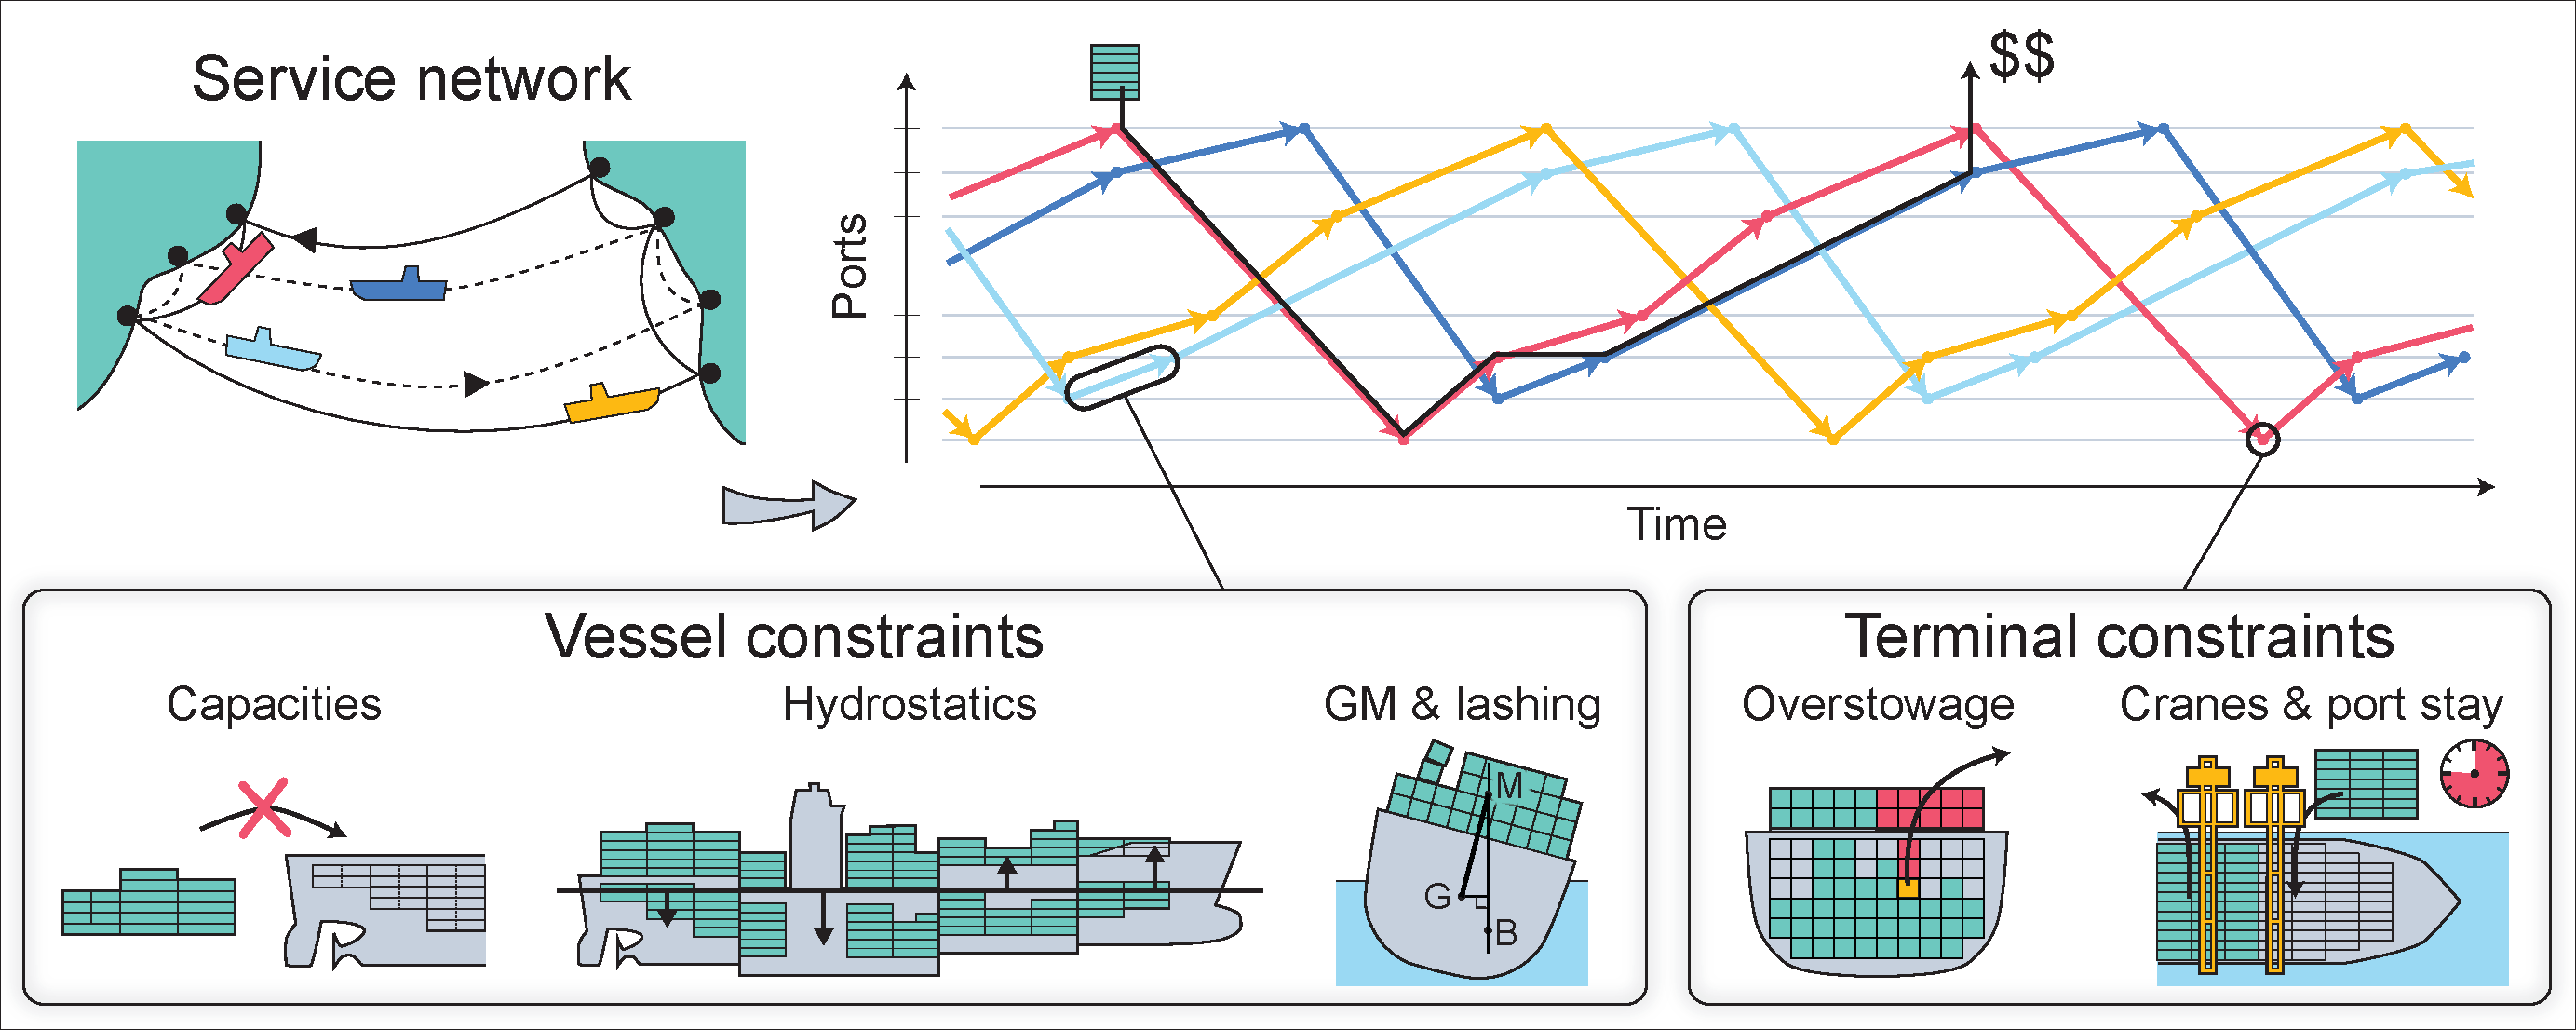
\includegraphics[width=13cm]{figures/abstract.pdf}
\end{graphicalabstract}

\begin{keywords}
Liner shipping\sep Revenue Management \sep Capacity Management \sep Cargo Allocation% \sep Operational Level Cargo Routing \sep Revenue Optimization
\end{keywords}

\maketitle


\section{Introduction}

Revenue Management (RM) is about providing customers with the right product at the right time and price. As an example, consider an airline operating a plane with 100 seats offering 50\% student discount. If the airline experiences that it can sell 80 tickets at full price, it should allocate 80 seats to these passengers and only offer them to students close to departure if the allocation cannot be filled.

Before the Liner Shipping (LS) conferences were outlawed in Europe in 2008, the lack of price differentiation gave carriers little reason to introduce RM methods. Since then it has been recognized that the industry has the core characteristics required for RM systems \cite{Hellerman06}: perishability of the product offered, relatively fixed capacity, low marginal sales cost and high marginal capacity change cost, ability to segment markets, sale or booking in advance, stochastic demand, and forecastable demand. This has lead to a growing body of literature on RM methods for LS and deployment of RM systems in the industry.

For RM methods to work in practice, though, it is important that it is possible at any time to accurately estimate the free capacity for each booking class. This is difficult for LS service networks due to operational constraints. The main challenge is to calculate the free cargo capacity of a vessel. A container slot on a cellular container vessel is different from a seat on an air plane and a hotel room. While a plane seat or a hotel room normally always is available if it is unused, a container slot can still be unavailable in this case. The reason is that a seaworthy vessel must comply with many interacting stowage rules and safety requirements. For instance, slots may be lost because the weight distribution otherwise would cause too high stress forces, insufficient transversal stability or too high draft. Moreover, slots in a single stack can be lost if the maximum weight of the stack or the maximum forces in the lashing gear otherwise are exceeded. The slot may also be lost for different types of containers: 20' containers cannot be stowed on top of 40' containers, refrigerated containers (reefers) must be near power plugs, and containers with dangerous cargo must be separated. In addition to vessel requirements, the capacity of service networks is affected by terminal constraints. A major challenge is to stay within the time window of a terminal call. This requires that crane moves of containers are distributed along the vessel such that a sufficient number of quay cranes can work in parallel to meet the time window. Since the cranes can only access containers from the top of the stacks, it is also important to avoid that containers for later ports block containers to be discharged below them. Such blocking containers must be restowed which take time and is costly \cite{JPAV18}.

None of the existing RM methods for LS that we are aware of model these operational constraints. Our collaboration with carriers over the last 15 years has given us insight in commercial work processes used by more than half of the market. The industry standard is to measure the free capacity of a container vessel in terms of: free volume in TEU~\footnote{Twentyfoot Equivalent Units.}, free weight in tons, and free number of plugs for refers. For instance, if a vessel has nominal capacity of 3,600 TEU, 45,000 tons, and 600 plugs, and currently has 2,500 TEU, 36,000 tons, and 350 reefers on board, then the free capacity according to this measure is 1,100 TEU, 9,000 tons, and 250 reefers. Some companies improve the measure by reducing it for each port of call according to its stowage team's {\em guaranteed intake} for this port. For instance, the stowage team may know that due to the typical cargo mix on board the vessel at departure from the port, they only succeed to use 3,300 TEU out of its nominal 3,600 TEU. Nevertheless, it is still a static average measure that does not take the actual cargo mix that was loaded in the port into account. Academic contributions of RM methods for LS use even simpler capacity models (see Section~\ref{sec:relatedwork}).

	In this article, we introduce an RM method for LS that to our knowledge is the first to include stowage and crane handling requirements. We consider the cargo flow in a service network over a time horizon and compute booking allocations or sales targets for the port calls in the network that maximize the total yield of loaded containers. Compared to similar previous work (e.g. Zurheide ...), we introduce operational constraints in the form of a vessel and terminal Standard Capacity Model (SCM). The vessel and terminal SCMs restrict the cargo flow on sailing and load/discharge arcs of the flow network, respectively. Both SCMs consist of linear constraints such that the resulting flow network is a linear program (LP) that can be solved efficiently with an of-the-shelf solver like CPLEX and COIN-OR (cite).
	The vessel SCM is an extension of a linear model of hydrostatic equilibrium introduced in \cite{ICCL18}. The paper includes an extensive experimental evaluation on real vessel data that shows that the model can predict draft, trim, and stress forces accurately. Our extensions to this model contribute:
\begin{itemize}

\item The first linear approximation of restows that we are aware of. Restow minimization is a well-known NP-hard problem (cite Tierney, Isreal). It has attracted more attention than any other stowage planning objective  (e.g., bla bla). For that reason, it is surprising that a rather simple yet strong linear approximation to date has been overlooked. 

\item The first linear approximation of lashing forces that we are aware of. It approximates non-linear but convex trade-offs between containers with different length and weight. 
  
\item A linear approximation of transversal stability (metacentric height) that uses regression analysis directly on the hydrostatic table. It avoids the fixed target displacement required in previous work (e.g., Pacino, Alberto).
  
\end{itemize}

The terminal SCM restricts the cargo flow in arcs in the network that represent load and discharge moves of cranes. Its major contributions are : 
\begin{itemize}

\item The first scalable model of cargo restowage. To our knowledge, only (botter) previously has represented where on the vessel restows are re-loaded. His (their?) Integer Programming (IP) model of this, however, is intractable.

\item A further development of the linear port stay model based on long cranes that was introduced by (pacino). Our model also takes the actual number of quay cranes available into account.    

\end{itemize}

We took six out of Maersk Line's seven Asian-Europe (AE) services in the fall 2018 and created a flow network over 90 days, where cargo was loaded in the first 45 days. We used real vessel data for a 15,000 TEU vessel. The resulting network had 296 port calls and each call was associated with a booking forecast defining a minimum amount to transport of each booking class (e.g., due to customer contracts) and a maximum amount achievable on the sport market. Yields for each booking class were derived from public freight rate data. The objective of the optimization was to find sales targets within the forecasted range maximizing the yield of loaded containers. The vessel SCM was adjusted to highest accuracy with 26 longitudinal sections. 

The network could be solved to optimality with CPLEX' barrier method in 23 minutes. The result had explicit operational parameters like stowage condition, trim, draft, crane work time etc. for all port calls and showed a 20\% lower yield compared to the nominal version of the three dimensional capacity model that is the industry standard in LS commercial decision making today.  

The results show a significant reduction of the available capacity when taking operational constraints into account. This is substantial in an industry with a profit margin of a few percent. Moreover, the results show that our LP flow network model is scalable even without using advanced methods like column generation. 

The rest of this article is organized as follows. Section XXX. ..
\input{relatedWork}
\section{Background}\label{sec:stowage}%Liner Shipping Operations
\subsection{Cargo and vessel}
Unsurprisingly, the cargo for container vessels consist for the most part of containers in standardized sizes. The most common sizes are 20' or 40' long containers with a width of 8' and a height of 8'6''. Containers with a length of 45', and containers with a height of 9'8'' also exists but are less common. Of these commonly sized container, some -- known as \emph{reefers} -- are used to transport goods that requires refrigeration, and these containers needs to be powered under transport.  The weight of the containers varies, but the cargo/containers are not uncommonly divided into weight classes denoted by an average weigth (for example, 5t, 13t, etc.).

The stowage area on a container vessel is divided into a grid of \emph{cells}, each of which can hold two 20' containers or one 40' (or 45') (see Figure~\ref{fig:vesselA}). Some of the cells have power plugs, which means that reefer containers can be stowed herein. 
Stacks of containers are arranged longitudinal in \emph{bays} consisting of stacks \emph{on deck} and \emph{below deck} (see Figure~\ref{fig:vesselA}), and each stack rests on sockets with a maximum weight limit. 
\emph{Hatch covers} separate the cargo on deck from the cargo below deck, and each hatch cover spans a number of bays in one direction and a number of stacks in the other direction (see Figure~\ref{fig:overstowA}).
For modelling purposes, the vessel is divided into \emph{sections} longitudinally consisting of zero or more bays together with the space in between (see Figure~\ref{fig:vesselA}). 

To help achieve stability of the vessel, large water ballast tanks are placed on the vessel (see Figure~\ref{fig:vesselA}). Other tanks containing e.g. bunker fuel and fresh water is also placed along the vessel.

\begin{figure}[pos=htbp]
	\centering
		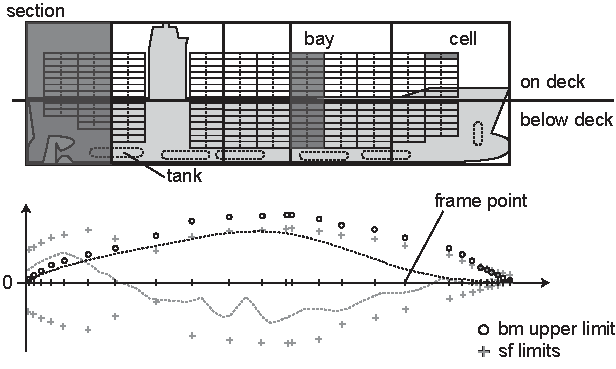
\includegraphics{figures/vessel1.pdf} 
	\caption{Vessel structure and limits for shear force (sf) and bending moment (bm) at frame points. The actual values of these forces are shown too \red{(but should they?)}.}
	\label{fig:vesselA}
\end{figure}

\subsection{Stowage considerations}
Stowing a container vessel is not as easy as it may sound initially, since many details regarding the cargo must be taken into consideration.
Below we will elaborate on some of these issues. The reader is referred to the recent book \cite{JPAV18} for more details.

%Capacity. 
Like with seats on an air-plane, there is a nominal upper bound on how many 20' and 40' containers, the stacks can hold. Likewise, only some of the cells have power plugs for reefer containers, limiting the number of these containers that can be stowed. These capacities are measured in \emph{twenty-foot equivalent units} (TEUs). 

%Hydrostatics. 
Though the number of containers is within the nominal capacities and the weight limits are also complied with, this does not guarantee the  seaworthiness of the vessel. When sailing, stress forces arise along the longitudinal axis of the vessel. These forces arise as a result of gravitation from the weight of cargo, tanks, and the vessel itself acting downwards and buoyancy from the water acting upwards. The resulting hydrostatic forces (stress forces, bending moments and transversal moments) must be within limits in order for the ship not to be impaired too much. These limits are given at certain positions along the vessel, known as \emph{frame points}. 

%GM and lashing (transversal stability).  
The metacentric height (GM) of a vessel is a measure relating to the transversal stability of the vessel against overturning. It is the distance between the center of gravity (G) of the vessel and the \emph{metacenter} M. M is found on a heeling vessel as the intersection of the centerline of the (transversally symmetric) vessel and a vertical line through the center of buoyancy (B) (see Figure~\ref{fig:GMA}). The higher GM is, the higher the transversal stability is (\cite{JPAV18}), and to avoid capsizing, it is therefore relevant to have this measure within given limits. 
On the other hand, GM affects other factors of stowing the vessel, e.g. lashing, where {higher} values of GM causes high acceleration forces \red{when the vessel is "correcting"}, meaning that less cargo can be securely stowed with lashing equipment. 

\begin{figure}[pos=htbp]
	\centering
	\begin{minipage}{.32\textwidth}
  %		\centering
  		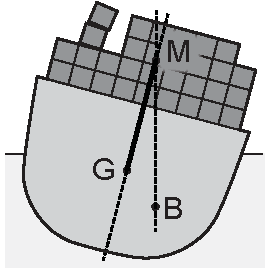
\includegraphics{figures/GM.pdf}
  		\caption{The metacentric heigh\\ (GM) of a heeling vessel.}
  		\label{fig:GMA}
	\end{minipage}%
	\begin{minipage}{.34\textwidth}
  	%	\centering
  		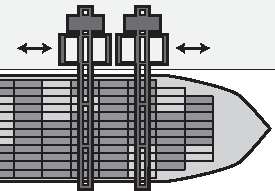
\includegraphics{figures/cranes.pdf}
  		\caption{Two cranes working on a\\ part of a vessel.}
  		\label{fig:cranes}
	\end{minipage}%
	\begin{minipage}{.34\textwidth}
  	%	\centering
  		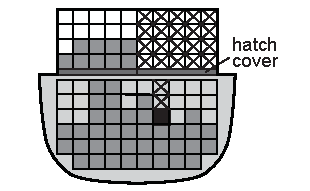
\includegraphics{figures/overstow.pdf}
		\caption{To move the black container,\\ the crossed out cells must be empty.}
  		\label{fig:overstowA}
	\end{minipage}
\end{figure}

%\begin{figure}[pos=htbp]
%\centering
%\begin{subfigure}[center]{.33\textwidth}
%  \centering
%  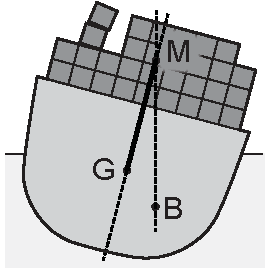
\includegraphics{figures/GM.pdf}
%  \caption{}
%  \label{fig:sub1}
%\end{subfigure}%
%\begin{subfigure}{.33\textwidth}
%  \centering
%  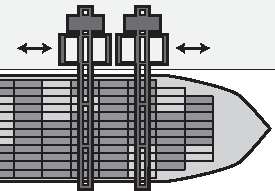
\includegraphics{figures/cranes.pdf}
%  \caption{}
%  \label{fig:sub2}
%\end{subfigure}%
%\begin{subfigure}{.33\textwidth}
%  \centering
%  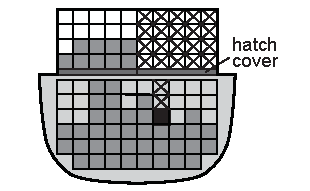
\includegraphics{figures/overstow.pdf}
%  \caption{}
%  \label{fig:sub3}
%\end{subfigure}
%\caption{\subref{fig:sub1} The metacentric heigh (GM) of a heeling vessel. \subref{fig:sub2} Two cranes working on a part of a vessel. \subref{fig:sub3} To move the black container, the crossed out cells must be empty.}
%\label{fig:test}
%\end{figure}
%
%\begin{figure}[pos=htbp]
%	\centering
%	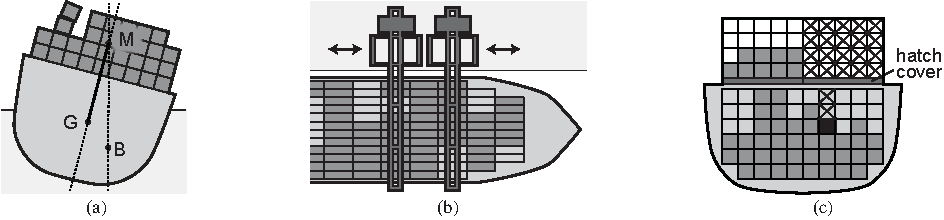
\includegraphics{figures/threefigs.pdf}
%	\caption{(a) The metacentric heigh (GM) of a heeling vessel. (b) Two cranes working on a part of a vessel. (c) To move the black container, the crossed out cells must be empty.}
%	\label{fig:GMA}
%\end{figure}

The circumstances at the ports where the cargo has to be loaded and discharged also has to be considered. 
The main concern here is the crane movements required to stow the vessel as planned/wanted, since crane movements both take time and have a cost associated. 
A crane operates at a bay at a time, and it takes time for it to move from one bay to another. Cranes cannot pass each other (i.e., they have to stay in the same order) and due to their size/width, they cannot work at adjacent bays (see Figure~\ref{fig:cranes}). The cranes operating on the vessel operate at the same time, but all crane movements have to be done within the time that the vessel is allotted at the port (or alternatively: the cost measured in time has to be considered, if time is unlimited). Thus, the crane taking the longest time should also be finished within the time frame.

Discharging any container cannot always be done with just one simple discharge move. When a container is discharged, there can be no containers on top of it, and if it is below deck, there can be no containers on the hatch cover above it (see Figure~\ref{fig:overstowA}). Thus, if a container below deck is topped by containers in this was \emph{that needs to stay on board}, then these containers have to be first unloaded and then loaded again. This is very expensive and time consuming, which should be reflected in the model. 

%\begin{figure}
%	\centering
%		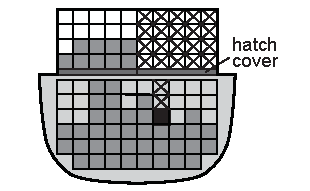
\includegraphics{figures/overstow.pdf}
%	\caption{To move the black container, the crossed out cells must be empty.}
%	\label{fig:overstowB}
%\end{figure}

When stowing, empty containers should be regarded as any other cargo, in the sense that they take up capacity and contribute to stress forces etc., and the moves that they give rise to should also be considered.    
\section{Model}\label{sec:model}

In this work, we consider a number of vessels that each sail with cargo between ports in two or more regions within a given time frame.  
The vessels' journeys can be illustrated in a network of \emph{port calls} as in Figure~\ref{fig:timespace}, where the horizontal axis illustrates time (the ordered set of \emph{dates}, $\mc{D}$, where port calls happens), while the vertical axis is made up by the set of \emph{ports} ($\mc{P}$). At a port call, cargo can be loaded to the vessel from the yard, or cargo can be discharged from the vessel to the yard. On the other hand, cargo at the yard of a port $p$ can be left at the yard until the next port call at $p$, as the dashed lines in Figure~\ref{fig:timespace} indicates. 

\begin{figure}[pos=htbp]
	\centering
		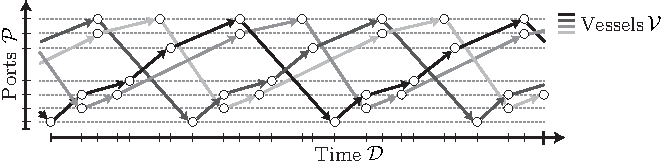
\includegraphics[scale = 1.3]{figures/netwBW2.pdf}
		\caption{A network of port calls showing four vessels sailing on routes between seven ports in two different regions.}  \label{fig:timespace}
\end{figure}

At each port call, containers can be exported from land, that is, it can be introduced to the yard at a port call, where it will eventually be picked up by a vessel. It is then transported through the network until it reaches its destination, where it is imported to land. At any port call on its way, it can be transshipped as described above. 
The first date in the network corresponds to the current state of the network, and hence there is already cargo on the vessels and possibly cargo at the yards of the ports.  

The network of port calls in Figure~\ref{fig:timespace} only gives a birds eye view of the flow graph $(\mc{N},\mc{E})$ that our model will be based on. In the detailed flow graph, each port call corresponds to a \emph{yard-side} node (in the set $\mc{N}^\ttt{y}\subset \mc{N}$) and a \emph{vessel-side} node (in the set $\mc{N}^\ttt{v}\subset\mc{N}$). This is illustrated in Figure~\ref{fig:flow} for a small network with only two services and only 6 port calls within the time frame of interest. The edges between the yard-side node and the vessel-side node correspond to loading and discharging of cargo between the vessel and the yard. The nodes $\mc{N}^\ttt{y}$ and $\mc{N}^\ttt{v}$ makes up the nodes of the flow network that are neither sources nor sinks. %Each of these nodes therefore has a port, a date, and a vessel associated with them.
Besides these nodes, $\mc{N}$ is comprised of the sources $I^\ttt{x}$, $I^\ttt{p}$, and $I^\ttt{v}$, denoting a common export node, a common source for the cargo at yards, and a common source for the cargo aboard the vessel, plus the sinks $O^\ttt{x}$, $O^\ttt{p}$, and $O^\ttt{v}$, which likewise are a common sink for import of cargo, cargo at yards after the last date within the time frame, and cargo on the vessel after the last date, respectively. See Figure~\ref{fig:flow}.

\begin{figure}[pos=htbp]
	\centering
		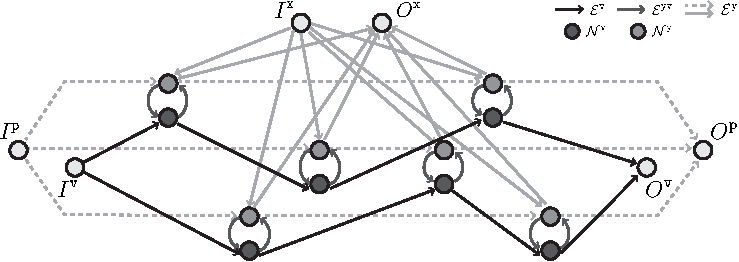
\includegraphics[scale = 1]{figures/fullFlow.pdf}
		\caption{Full flow network.}  \label{fig:flow}
\end{figure}

For convenience, we identify certain subsets of the edges, namely the \emph{sailing edges} $\mc{E}^\ttt{v}$ between a vessel-side node and another vessel-side node or the vessel sink/source, 
%$\mc{E}^{\ttt{v}}$, % =\set{(i,j)\in \mc{E}}{i,j\in \mc{N}^\ttt{v}\cup I^\ttt{v}\cup O^\ttt{v}}$,  
the \emph{terminal edges} $\mc{E}^\ttt{yv}$ between a vessel-side node and a yard-side node, 
%$\mc{E}^\ttt{yv}$, %=\{(i,j)\in \mc{E}\;|\;(i\in \mc{N}^\ttt{y}, j\in \mc{N}^\ttt{v}),$ $\text{ or } (i\in \mc{N}^\ttt{v}, j\in \mc{N}^\ttt{y})\}$, 
and the \emph{yard edges} $\mc{E}^{\ttt{y}}$ between a yard-side node and another yard-side node or the yard or cargo sink/source, 
%$\mc{E}^{\ttt{y}}$, % =\set{(i,j)\in \mc{E}}{i,j\in \mc{N}^\ttt{y}\cup I^\ttt{y}\cup O^\ttt{y}\cup I^\ttt{x}\cup O^\ttt{x}}$.
see Figure~\ref{fig:flow}.

Each vessel $v\in\mc{V}$ is divided into a number of \emph{sections}, and each section is divided into a \emph{subsection on deck} and a \emph{subsection below deck}, see Figure~\ref{fig:vessel}. We let $\mc{S}_v$ and $\mc{U}_v$ denote the set of sections and the set of all subsections, respectively, of the vessel $v\in \mc{V}$.
Cargo can be stowed in most (sub)sections, though, some sections might not contain any stowage area. Further, each section has ballast tanks available that can be filled with water to help distribute weight through out the vessel to keep it in hydrostatic balance.

\begin{figure}[pos=htbp]
	\centering
		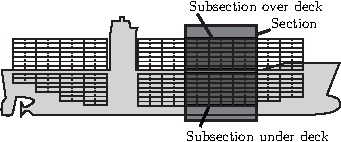
\includegraphics[scale = 1.2]{figures/vessel2.pdf}
		\caption{A section of a vessel and its subsections on and below deck.}  \label{fig:vessel}
\end{figure}

The cargo is divided into different \emph{container groups}, the set of which is denoted $\mc{G}$. Each group $g\in \mc{G}$ of containers has a type (that is, a length, a weight, and a reefer-property), a port of discharge, a deadline (a delivery date), and a yield. Some of the container groups have a deadline later than the last date in $\mc{D}$, while the remaining container groups, $\mc{G}'$, have a deadline in $\mc{D}$. Containers of a container group $g\in\mc{G}'$ must be delivered at the right destination if it is transported, and in this case, $N^g \in \mc{N}^\ttt{y}$ denotes the yard-side node of $g$'s destination port call.  

On sailing edges $e$, we want to know the amount of containers that are transported of a given container group in a particular subsection $u$ of the sailing vessel. Likewise, for terminal edges we want to know from/to which subsections, containers of each group are moved. This is recorded in the variables $x^g_{eu}$. For yard edges, there are no vessels associated and hence no positions on them to consider. In these cases, we only consider the number of containers of each container group that flows on the edge $e$, recorded in the variables $x^g_e$. Although these variables model integers,  we will ignore the integrality of them in our model due to the large number of containers.

In the following, we will describe the constraints of the model, before we finally introduce the considered objective function.
\subsection{Network flow constraints}\label{sec:flow}
 Table \ref{tab:net} summarizes the sets, variables and parameters, respectively, used to describe the flow model at a general level.

\begin{table}[width=.9\linewidth,cols=2,pos=htbp]%\begin{tabular*}{\tblwidth}{@{} Lp{11cm} @{}}
\caption{Sets, variables, and parameters used to describe the flow network.}\label{tab:net}
\begin{tabular*}{\tblwidth}{@{} Lp{10.8cm} @{}}
\toprule
$\mc{P}$, $\mc{D}$, $\mc{V}$		& Set of ports, dates, and vessels, respectively.\\
$\mc{S}_v$, $\mc{U}_v$				& Set of sections and set of all subsections, respectively, of the vessel $v\in\mc{V}$.\\ 
$\mc{G}$, $\mc{G}'\subset \mc{G}$	& Set of all container groups, and set of container groups that can be delivered within the given time frame.\\
$L=\{20,40\}$, $W$					& Set of lengths and weight classes, respectively, of container groups.\\
$\mc{N}, \mc{N}^\ttt{y}\subset \mc{N}, \mc{N}^\ttt{v}\subset \mc{N}$
									& Set of nodes, yard-side nodes, and vessel-side node, respectively. \\
$I^\ttt{x},I^\ttt{p},I^\ttt{v}, O^\ttt{x}, O^\ttt{p},O^\ttt{v}\in\mc{N}$
									& Sources (in-nodes) and sinks (out-nodes). \\
$\mc{E}$							& Set of edges in the flow graph.\\
$\mi{In}(i),\mi{Out}(i)\subset \mc{E}$	
									& Set of edges leading to, respectively from, the node $i\in\mc{N}$.\\
$\mc{E}^\ttt{yv}, \mc{E}^\ttt{v}, \mc{E}^\ttt{y}\subset\mc{E}$
									& Set of terminal edges, sailing edges, and yard edges, respectively.\\
$V_i, V_e\in\mc{V}$					& The vessel sailing to or from $i\in \mc{N}^\ttt{v}$ or being loaded/discharged at $i\in\mc{N}^\ttt{v}\cup\mc{N}^\ttt{y}$, and the vessel sailing at $e\in\mc{E}^\ttt{v}$ or being loaded/discharged at $e\in\mc{E}^\ttt{yv}$, respectively.\\ 
\midrule
$x^g_e\in\mathbb{R}^+_0$			& Number of containers of container group $g\in \mc{G}$ flowing on an edge $e\in \mc{E}^\ttt{y}\cup\mc{E}^\ttt{yv}$ to or from a yard-side node.\\
$x^{g}_{eu}\in\mathbb{R}^+_0$		& Number of containers of container group $g\in\mc{G}$ flowing on an edge $e\in\mc{E}^\ttt{v}\cup\mc{E}^\ttt{yv}$ to or from a vessel-side node in subsection $u\in \mc{U}_{V_e}$.\\
\midrule
$N^g\in\mc{N}^\ttt{y}$		 		& The yard-side node where a container group $g\in \mc{G}'$ should be imported.\\
$\mi{Ex}^{g\{+,-\}}_e\in\mb{N}_0$	
									& The minimal and maximal export, respectively, of container group $g\in \mc{G}$ at a yard-side node $i$, where $e=(I^\ttt{x},i)$.\\
$A^{g}_{eu}\in \mb{N}_0$			& The number of containers of container group $g\in\mc{G}$ in subsection $u\in \mc{U}_{V_e}$ of the vessel entering the network corresponding to the edge $e\in\mi{Out}(I^\ttt{v})$.\\
$A^g_e\in \mb{N}_0$					& The number of containers of container group $g\in \mc{G}$ that is at the yard of the port at the beginning of the network corresponding to the edge $e\in\mi{Out}(I^\ttt{p})$.\\
\bottomrule
\end{tabular*}
\end{table}

As a starting point, we model the flow of cargo in the time/space graph $(\mc{N},\mc{E})$. Preserving the flow of each group of containers at yard-side nodes results in constraint \eqref{OnOff}, while the flow preservation at vessel-side nodes is described in \eqref{secOnOff}. 
For the latter, we do not only consider the number of containers of each container group, but also the subsection at which the cargo is either placed or is moved to/from. Constraint \eqref{sumVars1} connects the variables without position information on the yard-side with variables with position information on the vessel-side. 

The export of each container group at a yard-side node has an upper and lower limit (\ref{exportLimits}), while it is given what is on board each vessel before the vessels reach their first port call in the network (\ref{onboard}), as well as what lies at each port before the first port call at a port (\ref{sourceYard}).

We ensure that everything that was initially on board the vessels, what was initially at the yards, and what is exported, is eventually imported at the right destination if this is possible, i.e. if the container group $g$ in question has a deadline within the given time frame ($g\in\mc{G}'$). Otherwise, the container group cannot be imported at a yard-side node in the considered network (both in \eqref{sinks}).  

\begin{alignat}{5}    
\label{OnOff}
\so[r]{\sum_{e\in \mi{In}(i)}} x^{g}_{e}	&= \so[r]{\sum_{e\in \mi{Out}(i)}}x^{g}_{e} &&\forall i\in \mc{N}^\ttt{y}, g\in \mc{G}\\
%
\label{secOnOff}
\so[r]{\sum_{e\in \mi{In}(i)}} x^{g}_{eu}	&= \so[r]{\sum_{e\in \mi{Out}(i)}}x^{g}_{eu}&& \forall i\in \mc{N}^\ttt{v}, u\in \mc{U}_{V_i}, g\in \mc{G} \\
%
\label{sumVars1}
x^g_{e} 									&= \sum_{u\in \mc{U}_{V_e}} x^{g}_{eu}		&& \forall e\in \mc{E}^\ttt{yv}, g\in\mc{G}\\
%
\label{exportLimits} \mi{Ex}^{g-}_e			&\leq x^g_{e}\leq \mi{Ex}^{g+}_e\quad		&& \forall e\in \mi{Out}(I^\ttt{x}), g\in \mc{G} \\
\label{onboard} 			x^{g}_{eu} 		&= A^{g}_{eu}								&& \forall e\in\mi{Out}(I^\ttt{v}), u\in \mc{U}_{V_e}, g\in \mc{G}\\
\label{sourceYard} 		x^g_{e} 			&= A^g_{e}									&& \forall e\in \mi{Out}(I^\ttt{p}), g\in \mc{G}
\end{alignat}

\begin{equation}\label{sinks}
x^g_{(i,O^\ttt{x})} = 
\left\{\begin{array}{rl}
		\quad\so[l]{\sum_{e\in\mi{Out}(I^\ttt{v})}}\so[r]{\sum_{u\in\mc{U}_{V_e}}} x^g_{eu} + \so[r]{\sum_{e\in \mi{Out}(I^\ttt{p})}} x^g_e + \so[r]{\sum_{e\in \mi{Out}(I^\ttt{x})}} x^g_{e}							 							 	& \text{if } g\in \mc{G}' \text{ and } i = N^g\\
													0	& \text{otherwise}\end{array}\right.				
\quad \forall i\in \mc{N}^\ttt{y}, g\in\mc{G}
\end{equation}

Besides the flow constraints, there are further capacity constraints of the flow graph $(\mc{N},\mc{E})$. These corresponds to vessel constraints (on sailing edges) that constrain the placement of cargo on the vessels when sailing, and terminal constraints (on terminal edges) that have to do with the loading and unloading of the vessel at the port calls. These constraints are collected in the \emph{standard capacity model for vessels}, $\mi{SCM}^\ttt{v}$, and the \emph{standard capacity model for terminals}, $\mi{SCM}^\ttt{t}$, respectively. We have chosen to not have any limitations on the yard-edges, which means that there is an unlimited storage capacity here. The model could, however, be easily expanded with constraints on those. 

The $\mi{SCM}^\ttt{v}$ is required to hold for all vessels when sailing, i.e. for all sailing edges $e\in\mc{E}^\ttt{v}$ \eqref{sailingCon}. The only relevant parameters for a model $\mi{SCM}^\ttt{v}_e$ are those pertaining to the vessel $V_e$ in question, and the only relevant variables for the model are what is on board the vessel in each of its subsections. Thus, the model is formulated using such parameters and variables, which is likewise expressed in \eqref{sailingCon}. 

The $\mi{SCM}^\ttt{t}$ applies to all port calls, which can be identified by a vessel side node $i\in \mc{N}^\ttt{v}$ \eqref{terminalCon}. The only relevant parameters for a model $\mi{SCM}^\ttt{t}_i$ are those pertaining to the vessel $V_i$ making the port call, and the only relevant variables for it are what was on board the vessel upon arrival at the port call of each container group at each subsection plus what is loaded and discharged from the vessel's subsections. As before, the model is therefore formulated using these variables and parameters only.    

The two models will be described in details in the sections below. When doing so, the two models are formulated using only the parameters and variables relevant to them. Their connections to the parameters and variables of the flow network is correspondingly expressed in \eqref{sailingCon} and \eqref{terminalCon}.

\begin{alignat}{3}
\label{sailingCon}
\mi{SMC}^\ttt{v}_e \text{ for all } e\in \mc{E}^\ttt{v}, \text{ where }\;
			&\left\{\;
			\begin{aligned}
					&x^g_{u\phantom{g}} = x^g_{eu} & \;\forall g\in\mc{G}, u\in \mc{U}_{V_e},\\
					&\mc{S} = \mc{S}_{V_e}, \mc{U} = \mc{U}_{V_e} 
			\end{aligned}\right.\\
%
\label{terminalCon}
\mi{SMC}^\ttt{t}_i \text{ for all } i\in\mc{N}^\ttt{v}, \text{ where } \;
			&\left\{\;
			\begin{aligned}
					&x^\ttt{at}_{gu} = x^g_{eu} && \;\forall g\in\mc{G}, u\in \mc{U}_{V_i}, e\in \mi{In}(i)\cap\mc{E}^\ttt{v},\\
					&x^\ttt{lo}_{gu} = x^g_{eu} && \;\forall g\in\mc{G}, u\in \mc{U}_{V_i}, e\in \mi{In}(i)\cap\mc{E}^\ttt{yv},\\
					&x^\ttt{di}_{gu} = x^g_{eu} && \;\forall g\in\mc{G}, u\in \mc{U}_{V_i}, e\in \mi{Out}(i)\cap\mc{E}^\ttt{yv},\\
					&\mc{S} = \mc{S}_{V_i}, \mc{U} = \mc{U}_{V_i} 
			\end{aligned}\right.
\end{alignat}

\subsection{Standard Capacity Model for vessels}
In constraint \eqref{sailingCon} above, $\mi{SCM}^\ttt{v}_{e}$ is a model that describe the feasible stowing of the vessel on each sailing edge $e\in \mc{E}^\ttt{v}$.  
The constraints on the sailing edges that our model take into account are vessel capacity constraints, hydrostatic constraints, and metacentric height and lashing constraints, which in turn will be described below. {A standard capacity model for vessels pertains to a given vessel, and in the following $\mc{S}$ and $\mc{U}$ will denote the sections and subsections, respectively, of the implicitly given vessel, that is, we leave out the subscript $e$.}
 
\subsubsection{Vessel capacity constraints}
Table~\ref{tab:capParams} summarizes the (not previously introduced) variables and parameters used to describe the vessel capacity constraints of the vessel of a sailing edge in the flow network.

\begin{table}[width=.9\linewidth,cols=2,pos=htbp]
\caption{Variables and parameters used for capacity constraints.}\label{tab:capParams}
\begin{tabular*}{\tblwidth}{@{} Lp{11cm} @{}}
\toprule
$x^g_u\in\mb{R}^+_0$				& Number of containers of container group $g\in \mc{G}$ that are stowed on the vessel in subsection $u\in \mc{U}$.\\
$w^{\ttt{ta}}_s\in\mb{R}^+_0$		& The weight of ballast tanks in section $s\in\mc{S}$.\\
\midrule
$\mc{G}^{20}, \mc{G}^{40}, \mc{G}^\ttt{r}\subset \mc{G}$ 
									& The set of container groups whose length is 20' and 40', respectively, and the container groups that are reefers.\\
$W^g\in {W}$, $T^g\in\{1,2\}$		& The weight of a container in container group $g\in \mc{G}$, and its number of TEUs.\\
$W^0_{s}\in\mb{R}^+$				& The constant weight (lightship) of section $s\in\mc{S}$.\\
$C^{\{{20},{40},\ttt{teu}, \ttt{rc}, \ttt{rp}\}}_u\in \mb{N}_0$  											
									& The capacities in TEU of subsection $u\in\mc{U}$ of 20' containers, 40' containers, total TEU, and reefers, and the number of reefer plugs in subsection $u\in \mc{U}$.\\
$C^{\{\ttt{w20}, \ttt{w}\}}_u\in\mb{R}^+_0$
									& The weight capacity of structures holding only 20' containers, and structures holding both 20' and 40' containers, of subsection $u\in\mc{U}$.\\
$L^{\ttt{ta}+}_s, L^{\ttt{disp}+}\in\mb{R}^+_0$
									& The upper limit for the weight of ballast tanks in section $s\in\mc{S}$, and the upper limit for the total displacement of the vessel.\\
\bottomrule
\end{tabular*}
\end{table}

In each subsection $u$ of a vessel there is limited stowage space (measured in TEU) that can hold 20' and 40' containers, respectively (\ref{cap20}), and there is a total TEU capacity \eqref{capTEU}. Likewise, the structures holding the containers can only withstand a certain force caused by the weight of the containers. Due to difference in where the forces of 20' and 40' containers apply - 40' containers only rest in structures with a distance of 40' while 20' containers rest on these and some structures in between - this results in constraints \eqref{cap20W} and \eqref{cap40W}.
Each subsection has a set number of reefer plugs that reefer containers need to use \eqref{caprp}, and the reefer containers need to be stowed in positions suited for this \eqref{caprc}.
Further, for each section, there is a limit on the amount of ballast water (in weight) used in tanks in that section of the vessel, and there is a upper limit on the displacement of the vessel in total, which consists of the constant weight of the vessel (lightship), the weight of ballast water and the weight of cargo \eqref{capDisp}.
\begin{alignat}{4}
&	\so[r]{\sum_{g\in \mc{G}^{l}}}T^gx^{g}_{u}\leq C^{l}_{u}   			&& \forall u\in \mc{U}, l\in L\label{cap20}\\
&	\so[r]{\sum_{g\in \mc{G}}}T^gx^{g}_{u} \leq C^\ttt{teu}_{u} 		&& \forall u\in \mc{U}\label{capTEU}\\
&	\so[r]{\sum_{g\in \mc{G}^{20}}}W^gx^{g}_{u}\leq C^\ttt{w20}_{u}    	&& \forall u\in \mc{U}\label{cap20W}\\
&	{\sum_{g\in \mc{G}}}\frac{1}{2}T^gW^gx^{g}_{u} \leq C^\ttt{w}_{u}	&& \forall u\in \mc{U}\label{cap40W}\\
&	\so[r]{\sum_{g\in \mc{G}^\ttt{r}}}x^{g}_{u}\leq C^\ttt{rp}_{u}		&& \forall u\in \mc{U}\label{caprp}\\
&	{\sum_{g\in \mc{G}^\ttt{r}}}T^gx^{g}_{u} \leq C^\ttt{rc}_{u} 		&& \forall u\in \mc{U}\label{caprc}\\
& w^{\ttt{ta}}_s \leq L^{\ttt{ta}+}_s									&& \forall s\in \mc{S}\label{capballast}\\
& \sum_{s\in\mc{S}}W^0_s + \sum_{s\in\mc{S}} w^\ttt{ta}_s + \sum_{g\in \mc{G}}\sum_{u\in\mc{U}}W^g x^g_u\leq L^{\ttt{disp}+}\quad \label{capDisp}
\end{alignat}

\subsubsection{Hydrostatic constraints}
When sailing, the vessel needs to be in hydrostatic balance, which the following constraints ensure. Table~\ref{tab:capParams} summarizes the sets, variables and parameters (not previously introduced) used to describe the imposed hydrostatic constraints. Details of this model can be found in \cite{iccl18}.

\begin{table}[width=.9\linewidth,cols=2,pos=htbp]
\caption{Sets, variables and parameters used for hydrostatic constraints.}\label{tab:hydro}
\begin{tabular*}{\tblwidth}{@{} Lp{12cm} @{}}
\toprule
$\mc{U}_s\subset\mc{U}$								& The subsections on and below deck of the section $s\in\mc{S}$.\\
$S^\ttt{bow}\in\mc{S}$								& The aft-most section in $\mc{S}$.\\
$S^\ttt{nx}_s\in\mc{S}$, $S^\ttt{a}_s\subset\mc{S}$	& The section next to $s\in\mc{S}\setminus S^\ttt{bow}$ in the aft direction, and all sections aft of $s\in\mc{S}$.\\
\midrule
$z^{\{\ttt{tr},\ttt{d}\}}\in\mathbb{R}$ 			& Trim and draft, respectively, of the vessel.\\
$z^{\{\ttt{b},\ttt{r}\}}_{s}\in \mathbb{R}$			& Buoyancy and resulting force, respectively, of section $s\in\mc{S}$.\\
$z^{\{\ttt{bm},\ttt{sf}\}}_{s}\in \mathbb{R}^+_0$	& Bending moment and shear force, respectively, at the aft endpoint of section $s\in\mc{S}$.\\
$w_{s} \in\mathbb{R}^+_0$							& The weight of cargo in section $s\in\mc{S}$.\\
\midrule
$L^{\{\ttt{tr},\ttt{d}\}\{+,-\}}\in\mb{R}$			& Upper and lower limits, respectively, for the trim and draft, respectively.\\
$L^{\{\ttt{sf},\ttt{bm}\}\{+,-\}}_{s}\in\mb{R}$		& Upper and lower limits, respectively, for the shear force and bending moment at the aft endpoint of section $s\in\mc{S}$.\\
$\Phi^{\{\ttt{d},\ttt{tr},\ttt{c}\}}_{s}\in\mb{R}$	& Linearization coefficients for the buoyancy of section $s\in \mc{S}$ w.r.t. draft, trim and a constant.\\
$\mi{Di}_{ss'}\in \mb{R}^+_0$						& The distance between the aft endpoint of section $s\in\mc{S}$ and the middle of section $s'\in\mc{S}$.\\
\bottomrule
\end{tabular*}
\end{table}

As described previously, a vessel is divided into a number of sections. When modeling the hydrostatics of a vessel on a sailing edge, we consider each of these sections and the forces acting on them separately. There is a gravitational force caused by the weight (including cargo) in section $s$, $w_{s}$, and there is a pull in the opposite direction, the buoyancy $z^\ttt{b}_{s}$, caused by the water displaced by the part of the vessel that is submerged in water \footnote{To simplify calculations, we do not multiply with the gravitational acceleration. Thus in reality, these variable actually denote weights and not forces, but this is, however, a common simplification.}. Subtracting the former from the latter, we get the resulting force on section $s$, $z^\ttt{r}_{s}$ \eqref{defResF}. 
The weight of a section consists of the constant weight, the weight of ballast, and the weight of cargo \eqref{defW}.
To find the buoyancy of a section, the area of submerged water for that section is linearized as a function of trim and draft (\ref{defBancy}). 
In short, the parameters for this linearization are found by modeling each section of the hull as rectangular boxes, which then makes it possible to calculate the submerged volume (and hence the buoyancy) given the draft (the mid-ship submersion) and trim (the tilt). The box-shapes are found by analysis of given vessel data and the linearization gives a good approximation of the buoyancy. For more details see \cite{iccl18}. 

We calculate the shear force and the bending moment at the aft end point of each section $s$. The shear force at the aft end point of section $s$ is the sum of resulting forces aft of the endpoint (\ref{defShear}). This is not calculated for the aft-most section $S^\ttt{bow}$. The bending moment at the aft end point of section $s$, on the other hand, equals the summation of the same terms, where each $z^\ttt{r}_{s'}$-term is multiplied with the distance from the aft end point of $s$ to the place where the resulting force act, i.e. the center of section $s$ (\ref{defBending}). Then we limit those forces by constants given in the input (\eqref{limitsShear} and \eqref{limitsBending}).
Due to hydrostatic equilibrium, there are no shear forces at the bow and stern, that is, the total buoyancy equals the total weight of the vessel (\ref{noShearAtEnds}).
Likewise there is no bending moment at the bow and stern, i.e. for the bow we get constraint \eqref{noMomentAtStern}.
					
The trim has a lower and upper limits \eqref{trimLimits}, and there is an upper and lower limit on the draft as well \eqref{draftLimits}, all of which might depend on where the vessel is sailing.
 
\begin{alignat}{3}    
& z^{\ttt{r}}_{s} = w_{s} - z^{\ttt{b}}_{s}									&& \forall s\in\mc{S} \label{defResF} \\
& w_{s} = W^{0}_{s} + w^{\ttt{ta}}_{s} + \sum_{g\in \mc{G}} \so[r]{\sum_{u\in \mc{U}_s}}W^g x^{g}_{u} \quad
																			&& \forall s\in\mc{S} \label{defW} \\
& z^{\ttt{b}}_{s} 	= \Phi^{\ttt{d}}_{s} z^\ttt{d} + \Phi^{\ttt{tr}}_{s} z^\ttt{tr} + \Phi^{\ttt{c}}_{s} 	
																			&& \forall s\in\mc{S} \label{defBancy} \\
%                                                                             
& z^{\ttt{sf}}_{s} 	= \sum_{s'\in S^\ttt{a}_s} z^{\ttt{r}}_{s'}				&& \forall s\in\mc{S}\setminus S^\ttt{bow} \label{defShear} \\
& z^\ttt{bm}_s 		= \sum_{s'\in S^\ttt{a}_s} \mi{Di}_{ss'} z^\ttt{r}_{s'}	&& \forall s\in\mc{S}\setminus S^\ttt{bow} \label{defBending} \\
& L^{\ttt{sf}-}_{s} \leq z^{\ttt{sf}}_{s} \leq L^{\ttt{sf}+}_{s}			&& \forall s\in\mc{S}\setminus S^\ttt{bow} \label{limitsShear} \\    
& L^{\ttt{bm}-}_{s} \leq z^{\ttt{bm}}_{s} \leq L^{\ttt{bm}+}_{s}  			&& \forall s\in\mc{S}\setminus S^\ttt{bow} \label{limitsBending}\\
& \sum_{s\in\mc{S}} (w_{s}-z^\ttt{b}_s)  = 0								&& \label{noShearAtEnds} \\
& \sum_{s\in\mc{S}} \mi{Di}_{S^\ttt{bow}s} z^{\ttt{r}}_{s} = 0				&& \label{noMomentAtStern}\\
%Limits
& L^{\ttt{tr}-}  	\leq z^\ttt{tr}    		\leq L^{\ttt{tr}+}				&& \label{trimLimits} \\
& L^{\ttt{d}-}	   	\leq z^\ttt{d}     		\leq L^{\ttt{d}+}				&& \label{draftLimits}
\end{alignat}

\subsubsection{Metacentric height and lashing constraints}
The metacentric height (GM) of a vessel is a measure relating to the stability of the vessel against overturning, and it is therefore relevant to have this measure within given limits. Further, GM affects other factors of stowing the vessel, e.g. lashing, where {higher} values of GM means that less cargo can be securely stowed with lashing equipment. In the following we describe the GM-related constraints in the $\mi{SCM}^\ttt{v}$. The variables and parameters used to describe these are summarized in Table~\ref{tab:gm}.

\begin{table}[width=.9\linewidth,cols=2,pos=htbp]
\caption{Sets, variables and parameters used to describe GM and lashing constraints.}\label{tab:gm}
\begin{tabular*}{\tblwidth}{@{} Lp{11.5cm} @{}}
\toprule
$\mc{U}^\ttt{o}$, $\mc{U}^\ttt{b}$	& The set of all subsection on deck, and all sections below deck, respectively.\\
\midrule
$z^{\ttt{gm}}\in\mathbb{R}$			&	GM of the vessel.\\
$w^{\ttt{ta}}, w^\ttt{o}, w^\ttt{b}\in\mathbb{R}^+_0$	
									&	The total weight of ballast tanks, the weight of cargo of all subsections in $\mc{U}^\ttt{o}$  and $\mc{U}^\ttt{b}$, respectively.\\
$\lambda^{\ttt{gm}\{+,-\}}_{u}, \lambda^{t\{+,-\}}_{u}\in\mathbb{R}^+_0$ 
									&	Coefficients for a convex combination describing allowable lashing combinations for subsection $u\in \mc{U}^\ttt{o}$ and containers with a given length and weigth $t\in L\times W$.\\
\midrule
$\mc{G}^t$							& The container groups that have a specified length and weight $t\in L\times W$.\\
$\Psi^{\{\tt{o},\ttt{b},\ttt{ta},\ttt{d},\ttt{tr},\ttt{c}\}}\in\mb{R}$	
									& Linearization coefficients for the GM of the vessel w.r.t. the weight of cargo on deck, the weight below deck, the weight of ballast tanks, the draft, the trim, and a constant.\\
$N^{t\{+,-\}}_{u}\in\mb{N}_0$		& Maximal number of containers with length and weight $t\in L\times W$ that can be put in subsection $u\in \mc{U}^\ttt{o}$ on deck when the vessel assumes the minimal and maximal GM-value, respectively.\\
$L^{\ttt{gm}\{-,+\}}\in\mb{R}^+_0$ 	& Upper and lower limit for GM.\\
\bottomrule
\end{tabular*}
\end{table}
 
Firstly, GM depends on the center of gravity of the vessel. We have here assumed that GM can be approximated by a linear function over the weight (of cargo) on deck, the weight (of cargo) below deck, the weight of tanks/ballast water, the draft, and the trim of the vessel. Therefore, we have constants $\Psi^{\ttt{o}}$, $\Psi^{\ttt{b}}$, $\Psi^{\ttt{ta}}$, $\Psi^{\ttt{tr}}$, $\Psi^{\ttt{d}}$, $\Psi^{\ttt{c}}$ for expressing this linear relationship in \eqref{defGM}. This linear equation uses defined variables denoting the weight of cargo on deck, below deck, tanks, trim and draft. The former three variables are defined in \eqref{defWo}, \eqref{defWu}, and \eqref{defWT}, respectively, while the latter two are implicitly defined in the equation system \eqref{defResF}-\eqref{draftLimits}. There is a minimum and a maximum value for GM (\ref{minGM}). %[Might not be the same as $L^{GM-}$ though].

The mentioned constants for the linearization of GM have been found by a linear regression over app. 3000 data points. % = 2985
The generation of these data points and a discussion of the accuracy are described in Section~\ref{sec:implementation}. 

\begin{alignat}{3}    
&z^{\ttt{gm}} 	= \Psi^{\ttt{o}}\cdot w^\ttt{o} + \Psi^{\ttt{b}}\cdot w^\ttt{b} + \Psi^{\ttt{ta}} \cdot w^\ttt{ta}
+ \Psi^{\ttt{d}} \cdot z^{\ttt{d}} + \Psi^{\ttt{tr}} \cdot z^{\ttt{tr}} + \Psi^{\ttt{c}}\quad			\label{defGM}\\
%
&w^\ttt{o} 		= \sum_{u\in \mc{U}^\ttt{o}}\sum_{g\in \mc{G}} W^g x^{g}_{u}	 						\label{defWo} \\
&w^\ttt{b} 		= \sum_{u\in \mc{U}^\ttt{b}}\sum_{g\in \mc{G}} W^g x^{g}_{u} 							\label{defWu} \\
%
&w^\ttt{ta} 	= \sum_{s\in\mc{S}} w^{\ttt{ta}}_{s} 													\label{defWT} \\
%
&L^{\ttt{gm}-} 	\leq z^{\ttt{gm}}	\leq L^{\ttt{gm}+}													\label{minGM}
\end{alignat}    

GM affects the stability of the vessel and hence also how much cargo can be safely lashed on deck. For given minimal and maximal GM-values ($L^{\ttt{gm}-}$ and $L^{\ttt{gm}+}$), the maximal number of containers that can be stowed in a subsection $u\in \mc{U}^\ttt{o}$ on deck of containers with a given length and weight $t\in L\times W$ has been determined ($N^{t+}_{s}$ and $N^{t-}_{s}$). The more containers of other length-weight combinations, the less containers of a given length-weight can be safely lashed above deck. 
In a space with a dimension for each $t\in L\times W$ plus a dimension for GM, we make a polygon describing the allowable cargo-combinations (w.r.t. lashing) of subsection $u\in\mc{U}^\ttt{o}$ as GM varies. For the minimal GM-value, the polygon has a corner in each $t$-dimension at $N^{t-}_{s}$ and at $\bar{0}$, and similarly for the maximal GM-value (see Figure~\ref{fig:GMpolygon}). %The internal points of the polygon describes allowable configurations of cargo when the vessel has a specific GM. 
An allowable configuration will be a convex combination of the corner points in the polygon. %, $\sum_{(l,w)\in \mc{Q}\times \mc{W}}\lambda^{lw-}_{sij} \bar{C^{lw-}}_{sij} + \lambda^{\ttt{gm}-}_{sij}L^{\ttt{gm}-} + \lambda^{\ttt{gm}+}_{sij}L^{\ttt{gm}+}$. 
For the GM-dimension, the convex combination results in \eqref{convexGM1} below. For any other dimension, since each corner point's coordinate is zero in all dimensions except for the $t$-dimension in question (where it is either $N^{t+}_{s}$ or $N^{t-}_{s}$) and the GM-dimension (where it is either $L^{\ttt{gm}+}$ or $L^{\ttt{gm}-}$), this leads to the constraint \eqref{convexGM2}.  \eqref{lambdaSum} and \eqref{positiveLambdas} says that this linear combination is convex. 

\newsavebox{\smlmat}% Box to store smallmatrix content
\savebox{\smlmat}
{	$\mathbf{x} = \lambda^{t_1-}_u\left(\begin{smallmatrix}N^{t_1-}_u\\0\\L^{\texttt{gm}-}\end{smallmatrix}\right)
	+ \lambda^{t_1+}_u\left(\begin{smallmatrix}N^{t_1+}_u\\0\\L^{\texttt{gm}+}\end{smallmatrix}\right)
+ \lambda^{t_2-}_u\left(\begin{smallmatrix}0\\N^{t_2-}_u\\L^{\texttt{gm}-}\end{smallmatrix}\right)
+\lambda^{t_2+}_u\left(\begin{smallmatrix}0\\N^{t_2+}_u\\L^{\texttt{gm}+}\end{smallmatrix}\right)
+\lambda^{\texttt{gm}-}_u\left(\begin{smallmatrix}0\\0\\L^{\texttt{gm}-}\end{smallmatrix}\right)
+\lambda^{\texttt{gm}+}_u\left(\begin{smallmatrix}0\\0\\L^{\texttt{gm}+}\end{smallmatrix}\right)$
}

\begin{figure}[pos=htbp]
	\centering
		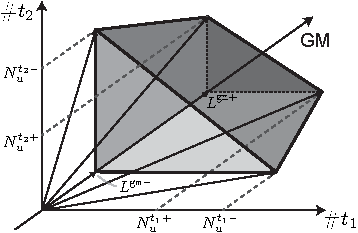
\includegraphics[scale=1]{figures/GMpolygon.pdf}
	\caption{Polygon of legal combinations of container types. $\mathbf{x}$ is a convex combination of the shown vectors.}
%	\usebox{\smlmat}
	\label{fig:GMpolygon}
\end{figure}

The values $N^{t+}_{s}$ or $N^{t-}_{s}$ were found by use of a professional loading computer as described in Section~\ref{sec:implementation}. This section also includes a discussion of the validity of this approach. 

\begin{alignat}{3}    
\label{convexGM1}
& z^\ttt{gm} = L^{\ttt{gm}-}\lambda^{\ttt{gm}-}_{u}+L^{\ttt{gm}+}\lambda^{\ttt{gm}+}_{u} + \sum_{t\in L\times W}(L^{\ttt{gm}-}\lambda^{t-}_{u} + L^{\ttt{gm}+}\lambda^{t+}_{u})\quad 																																			&& \forall u\in \mc{U}^\ttt{o} \\
\label{convexGM2}
&\smashoperator[r]{\sum_{g \in \mc{G}^{t}}} x^{g}_{u} = N^{t-}_{u} \lambda^{t-}_{u} + N^{t+}_{u} \lambda^{t+}_{u}\quad			&& \forall u\in \mc{U}^\ttt{o}, t\in L\times W\\
\label{lambdaSum} 
& \lambda^{\ttt{gm}-}_{u}+\lambda^{\ttt{gm}+}_{u} + \so[r]{\sum_{t \in L\times W}}(\lambda^{t-}_{u} + \lambda^{t+}_{u}) = 1 	&& \forall u\in \mc{U}^\ttt{o}\\
\label{positiveLambdas}
&\lambda^{\ttt{gm}+}_{u}\geq 0,	\lambda^{\ttt{gm}-}_{u}\geq 0, \lambda^{t+}_{u}\geq 0, \lambda^{t-}_{u}\geq 0					&& \forall u\in \mc{U}^\ttt{o}, t\in L\times W
\end{alignat} 

\subsection{Standard Capacity Model for terminals}
\begin{figure}[pos=htbp]
	\centering
		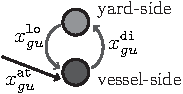
\includegraphics[scale=1]{figures/terminalVars.pdf}
	\caption{Variables used for terminal constraints}
	\label{fig:terminalVars}
\end{figure}

In constraint \eqref{terminalCon} of Section~\ref{sec:flow}, $\mi{SCM}^\ttt{t}_{i}$ is a model restricting the actions taking place at the port call associated with the vessel-side node $i\in \mc{N}^\ttt{v}$.
The model includes overstowage and port stay constraints and will be described in the following. For describing the terminal constraints, we need variables describing what is on board the vessel upon arrival at the port call, as well as what is loaded and what is discharged, see Figure~\ref{fig:terminalVars}. The vessel in question is implicitly given.



The new variables and parameters used for the terminal constraints are summarized in Table~\ref{tab:portStay}. %\red{In red: has already been defined, but for vessel constraints.}

\begin{table}[width=.9\linewidth,cols=2,pos=htbp]
\caption{Variables and parameters for terminal constraints.}\label{tab:portStay}
\begin{tabular*}{\tblwidth}{@{} Lp{11.8cm} @{}}
\toprule
${U}^\ttt{o}_s, {U}^\ttt{b}_s \in \mc{U}$	%{$\mc{U}_s\subset\mc{U}$},
									& %The subsection of section $s\in\mc{S}$, and t
									The subsections of section $s\in \mc{S}$ that is on deck and below deck, respectively.\\
%\red{$S^\ttt{bow}\in\mc{S}$, $S^\ttt{nx}_s\in \mc{S}$}		
%									& The aft-most section, and the section next to section $s\in\mc{S}\setminus S^\ttt{bow}$ in the aft direction.\\
\midrule
$x^\ttt{at}_{gu}$, $x^\ttt{lo}_{gu}$, $x^\ttt{di}_{gu}\in\mb{R}^+_0$
									& The number of containers of type $g\in \mc{G}$ that is on board the vessel in subsection $u\in\mc{U}$ upon arrival, that is loaded to $u$, and that is discharges from $u$, respectively.\\
$z^\ttt{mo}_{ls}\in\mathbb{R}^+_0$	& Total number of load and discharge moves of containers of length $l\in L$ in section $s\in\mc{S}$.\\					
$z^{\ttt{ps}}\in\mathbb{R}^+$ 		& Minimal length of the port stay.\\
\midrule
%\red{$\mi{C}^\ttt{teu}_u\in \mb{N}^+_0$} 
%									& The TEU capacity of subsection $u\in \mc{U}$.\\
$\mi{Cr}\in\mb{N}$					& The number of cranes available at the port call.\\
$\mi{Cm}^{l}\in\mb{R}^+$			& The number of containers of length $l\in L$ that can be moved per crane per hour.\\
$B_{s}\in \mb{N}_0$					& The number of bays in section $s\in \mc{S}$.\\
$L^{\ttt{ps}+}\in\mb{R}$			& Maximal port stay for the port call.\\
\bottomrule
\end{tabular*}
\end{table}

\subsubsection{Overstowage}
When cargo is unloaded at a port call of a port $p$, sometimes cargo in a subsection on deck (destined to another port than $p$) blocks some of the cargo below deck that needs to be discharged at $p$. That is, the cargo on deck \emph{overstowes} the cargo below deck. In that case, the cargo on deck also has to be discharged (and most likely re-loaded to the vessel), and this is unnecessary and costly operations. 
Since our model only know the position of cargo in subsections of the vessel, we cannot make an exact calculation of the overstowage, however, we can make a conservative lower bound of the number of containers on deck that has to be discharged in order to discharge the needed cargo below deck. 

\begin{figure}[pos=htbp]
	\centering
		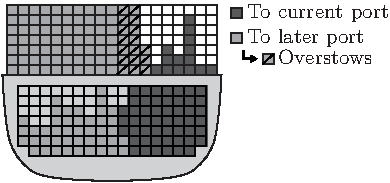
\includegraphics[scale=1]{figures/overstowage.pdf}
	\caption{Only the shaded containers overstow containers below deck.}
	\label{fig:overstow}
\end{figure}

In the best case scenario (w.r.t. overstowage), in a section $s$ the cargo below deck that will be unloaded at $p$ fills stowage space below deck from one side (e.g. starboard) while the cargo on deck fills the stowage space on deck from the other side (port side). Disregarding the hatch covers, we then only need to unload the ``overlapping'' part of the cargo above deck (see Figure~\ref{fig:overstow}).
In the best case, this cargo needs to be unloaded and imported at the port.  
The constraint do not take hatch covers into account, and we likewise do not take into account that the stowage area on deck might span a wider area (from starboard to port) than the stowage area below deck. However, we normalize with respect to the TEU capacity of the relevant subsections on and below deck \eqref{overst}. 
Notice that our model do not require that this cargo is put back at the same place, though this is possible to impose as a constraint.

\begin{eqnarray}
\label{overst}
\sum_{g\in \mc{G}} \frac{T^g}{C^\ttt{teu}_{U^\ttt{o}_s}}x^\ttt{di}_{gU^\ttt{o}_s} \geq \sum_{g\in \mc{G}}\frac{T^g}{C^{\ttt{teu}}_{U^\ttt{o}_s}}x^\ttt{at}_{gU^\ttt{o}_s} + \sum_{g\in \mc{G}}\frac{T^g}{C^{\ttt{teu}}_{U^\ttt{b}_s}}x^\ttt{di}_{gU^\ttt{b}_s} - 1\quad
																																										&\forall s\in\mc{S}\;.\;C^{\ttt{teu}}_{U^\ttt{o}_s}\neq 0, C^{\ttt{teu}}_{U^\ttt{b}_s}\neq 0
\end{eqnarray}

\subsubsection{Crane moves and port stay}
Loading and discharging cargo to/from a vessel requires crane operations that takes time. The number of 20'- and 40'-containers being loaded to or from a section $s$ of the vessel is defined in \eqref{defMoves}. Given the number of 20-moves (40 moves) that a crane can do per hour, $\mi{Cm}^{20}$ ($\mi{Cm}^{40}$), plus the number of cranes at the corresponding port call, $\mi{Cr}$, we can calculate the least amount of time, the port call will last (i.e., the port stay, denoted by the variable $z^\ttt{ps}$) (\ref{minPortStay}).  

Due to the width of the cranes, two cranes cannot operate at the same time on two immediately adjacent bays. This means, that for any pair of adjacent bays, a crane will first work on one of the bays, and then the same or another crane will work on the other bay. So the port stay will at least last as long as it takes to work on any pair of adjacent bays, called the \emph{long crane}. However, the port stay must be done within the time window for the port call ($L^{\ttt{ps}+}$) (\ref{maxPs}). Since a section of the vessel can contain more than one bay, we make a conservative estimate; the least constraining distribution of cargo (w.r.t. crane operating time) is if the cargo is distributed evenly in each section. Operating on two bays in a section is then estimated by \eqref{longCrane}. If a section only contains one bay, a lower bound for the operating time on this section and an adjacent section is given in \eqref{longCrane1Bay}.

\begin{alignat}{4}
\label{defMoves}
&z^\ttt{mo}_{ls} = \sum_{u\in \mc{U}_{s}}\sum_{g\in \mc{G}^l}(x^\ttt{lo}_{gu} + x^\ttt{di}_{gu}) 
																						&&\forall l\in L, s\in \mc{S}\\
\label{minPortStay}
&z^{\ttt{ps}} \geq \sum_{l\in L}\sum_{s\in\mc{S}} \frac{1}{\mi{Cr}\cdot \mi{Cm}^{l}}\cdot z^\ttt{mo}_{ls} \\
%
\label{maxPs}
& z^\ttt{ps}\leq L^{\ttt{ps}+}\\
%																							
\label{longCrane}
&z^{\ttt{ps}} \geq \sum_{l\in L}\frac{2}{B_{s}\cdot \mi{Cm}^{l}}\cdot z^\ttt{mo}_{ls}	&& \forall s\in\mc{S}. B_s > 1\\
%
\label{longCrane1Bay}
&z^\ttt{ps} \geq \sum_{l\in L}\frac{1}{B_s\cdot \mi{Cm}^l} z^\ttt{mo}_{ls} + \sum_{l\in L}\frac{1}{B_{S^\ttt{nx}_s}\cdot \mi{Cm}^{l}} z^\ttt{mo}_{lS^\ttt{nx}_s}\quad	
																						&& \forall s\in\mc{S}\setminus S^\ttt{bow}. B_s = 1 \text{ or } B_{S^\ttt{nx}_s} = 1
\end{alignat}

\subsection{Objective function}
In this model we want to optimize the yield given by the containers being exported in the network from which we subtract the costs given by crane operations, costs associated with sailing long legs (legs between ports in different regions) with filled ballast tanks, and costs associated with storing containers at a yard. This is modelled in \eqref{obj}, where $Y^g$ is the yield associated with container group $g\in\mc{G}$, $D_e$ is the number of days between the port calls at the start and end of edge $e\in \mc{E}^\ttt{y}$, $\mc{E}^\ttt{long}\subset\mc{E}^\ttt{v}$ are \emph{long legs}, i.e. sailing edges between ports in two different regions, while $\mi{Co}^g_{e}$, $\mi{Co}^\ttt{ta}$, $\mi{Co}^{\ttt{mo}l}$, respectively are the costs associated with storing one container of container group $g\in\mc{G}$ at the yard of the port calls in the start and end of edge $e\in\mc{E}^\ttt{y}$ for one day, the costs of sailing with one ton of ballast on a long leg, and the cost of moving (loading or discharging) one container of length $l\in L$, respectively. These set and parameters are summarized in Table~\ref{tab:obj}. {We notice that the variable $z^{\texttt{mo}}_{lis}$ is the variable $z^\texttt{mo}_{ls}$ defined in \eqref{defMoves} for the port call at the implicitly given vessel-side node $i$.}

\begin{table}[width=.9\linewidth,cols=2,pos=htbp]
\caption{set and parameters used in the objective function.}\label{tab:obj}
\begin{tabular*}{\tblwidth}{@{} Lp{11.8cm} @{}}
\toprule
$\mc{E}^\ttt{long}\subset\mc{E}^\ttt{v}$ & Sailing edges between ports in two different regions.\\
\midrule
$Y^g$ 		& The yield associated with container group $g\in\mc{G}$.\\
$D_e$ 		& Number of days between the port calls corresponding to the edge $e\in\mc{E}^\ttt{y}$.\\
$\mi{Co}^g_e$, $\mi{Co}^\ttt{ta}$, $\mi{Co}^{\ttt{mo}l}$ 
			& Costs associated with storing one container of container group $g\in\mc{G}$ at the yard of the port of the edge $e\in\mc{E}^\ttt{y}$ for one day, the costs of sailing with one ton of ballast on a long leg, and the cost of moving (loading or discharging) one container of length $l\in L$, respectively.\\
\bottomrule
\end{tabular*}
\end{table}

\begin{equation}\label{obj}
\sum_{g\in\mc{G}}\so[r]{\sum_{e\in\mi{Out}(I^\ttt{x})}}Y^g x^g_{e} 
- \sum_{g\in\mc{G}}\so[r]{\sum_{e\in \mc{N}^\ttt{y}\times\mc{N}^\ttt{y}}} \mi{Co}^g_e D_e x^g_e 
- \so[r]{\sum_{e\in\mc{E}^\ttt{long}}} \mi{Co}^\ttt{ta} w^\ttt{ta}_e 
-\sum_{i\in \mc{N}^\ttt{v}}\sum_{s\in\mc{S}_{V_i}}\sum_{l\in L} \mi{Co}^{\ttt{mo}l} z^{\ttt{mo}}_{lis}
\end{equation}

\input{issues}
\section{Results/Numerical Experiments}
In the following, we first look at groups of constraints individually and conduct experiments to show their impact. Then we look at results for a full-scale, realistic network of port calls and perform some scaling experiments. %An illustration of the key number that our model can show, is illustrated for a small network in the appendix. 

For all of the following experiments, $L=\{20,40\}$ and $W = \{5,13,19,26\}$, and $T=L\times W\times \{\text{R},\text{NR}\}$ is the set of considered types of a container group. We use a vessel with 23 bays, and we {divide the vessel in up to 26 sections (i.e., $|S| = 26$ )} each spanning one or zero bays. The sections that cannot contain cargo are included to improve precision of hydrostatic constraints. Non-ballast tanks are assumed filled 70\%.

In the experiments, we compare with a so-called simple model, which is a vessel capacity model that takes into account the total TEU capacity, the total reefer capacity, and the total displacement (corresponding to the constraints \eqref{capTEU}, \eqref{caprc}, and \eqref{capDisp} for the single section including the whole vessel).


\subsection{Vessel constraints} % (single-ship optimizations)
Our first series of experiments look at the vessel constraints separately, i.e. we consider the constraints defining $\mathit{SCM}^\ttt{v}_{e}$ in \eqref{sailingCon} for a single sailing edge $e$. 
For all experiments in this section, $|S| = 26$.
Since we only consider a single vessel in these experiments, we do not consider all the properties of container groups (e.g., the destination port is irrelevant). Thus, in the following experiments, we only refer to the type of a container group, i.e. the length, the weight class and whether it is a reefer container or not. 

\subsubsection{Vessel capacity constraints and hydrostatic constraints}
To investigate the impact of the vessel capacity constraints (constraints \eqref{cap20}-\eqref{capDisp}), we find the maximal number of containers of a type $t\in T$ that can be placed on a vessel with a given ROB cargo. This number is found in the case where all vessel capacity constraints are enforced, and in the case when only 3 basic constraints capcity are considered are enforced (the simple model described above).
The ROB cargo is constructed with heavy cargo in the fore- and aft-most horizontal sections while it is empty in the middle horizontal sections. It is given in Table~\ref{tab:ROBCap} and shows the number of each type of container in non-empty bays, on and below deck.

\begin{table}[width=.9\linewidth,cols=11,pos=htbp]
\caption{ROB cargo for experiment with vessel capacity constraints and hydrostatic constraints.}\label{tab:ROBCap}
\begin{tabular*}{\tblwidth}{@{} R *{10}C @{}}
\toprule
&\multicolumn{10}{c}{Bay (on deck-below deck)}\\
\cmidrule{2-11}
Container type&1&2&3&4&5&19&20&21&22&23\\
\midrule
40', 26t, NR &  70-28 & 105-60 & 80-100& 90-115& 90-135& 72-0 & 42-132 & 42-110 & 33-92 & 33-24\\

\bottomrule
\end{tabular*}
\end{table}

The results of the optimizations are given in Table~\ref{tab:resultsCap}, where also the overestimation (O.e.) is shown given in percentage of the more constrained model. 
\\\\
To investigate the effects of the hydrostatic constraints, we have made two similar experiments. First we use a model with vessel capacity constraints and hydrostatic constraints (constraints \eqref{cap20}-\eqref{draftLimits}), where ballast tanks can be filled freely within the upper limits. Again we optimize the number of containers of each type that can be placed on the vessel with the given ROB. Afterward, the optimizations are repeated where we further require that the tanks are left empty, which might be a reasonable requirement on long legs in order to prevent wear and tear.
 
The results are shown in Table~\ref{tab:resultsCap} as  well as the overestimation (O.e.) of a model compared to a more constrained model. This overestimation is given in percentage of the objective value of the more constrained model and is shown in a column between the two models being compared.

%
\begin{table}[width=.95\linewidth,cols=10,pos=htbp]
\caption{Maximal number of containers of each type that can be placed on the vessel, when vessel capacity constraints and hydrostatic constraints are/are not included, respectively. The columns marked ``O.e.'' indicates the overestimation between the two models on either sides. }\label{tab:resultsCap}
\begin{tabular*}{\tblwidth}{@{} r@{\hskip3pt}r@{\hskip3pt}r *{7}{R} @{}}
\toprule
&&&\mult{7}{c}{Included constraints}\\
\cmidrule{4-10}
	&	 &	&		 &		&		   &		&Capacities,  &		  &Capacities,\\		
	&	 &	& 		 &		&Capacities&		&hydrostatics,&	    &hydrostatics,\\	
\mult{3}{c}{Type}
				     &	Simple &O.e.   &(No tanks)&O.e.&tanks free   &O.e. &tanks empty	\\		
\midrule
20',& 5t,&NR& 12802.0& 14.8 & 11151.6  & 6.7& 10450.1 		& 19.4&  8751.3\\
20',& 5t,& R&  2024.0& 31.3 &  1542.0  & 0.0&  1542.0 		&  0.0&  1542.0\\
20',&13t,&NR&  7900.9& 0    &  7900.9  & 3.2&  7658.3 		&  0.0&  7658.3\\
20',&13t,& R&  2024.0& 31.3 &  1542.0  & 0.0&  1542.0 		&  0.0&  1542.0\\
20',&19t,&NR&  5405.9& 0    &  5405.9  & 1.6&  5322.3 		&  0.1&  5319.0\\
20',&19t,& R&  2024.0& 33.0 &  1522.2  & 1.6&  1498.6 		&  0.0&  1498.6\\
20',&26t,&NR&  3950.5& 0    &  3950.5  & 1.6&  3889.4 		&  0.1&  3887.0\\
20',&26t,& R&  2024.0& 53.5 &  1318.3  & 1.8&  1295.5 		&  0.0&  1295.5\\
40',& 5t,&NR&  6401.0& 0.3  &  6379.0  &15.7&  5513.1 		& 19.6&  4608.6\\
40',& 5t,& R&  2024.0& 118.8&   925.0  & 0.0&   925.0 		&  0.0&   925.0\\
40',&13t,&NR&  6401.0& 2.3  &  6255.0  & 9.5&  5713.8 		& 14.6&  4985.7\\
40',&13t,& R&  2024.0& 118.8&   925.0  & 0.0&   925.0 		&  0.0&   925.0\\
40',&19t,&NR&  5405.9& 0    &  5405.9  & 4.1&  5191.6 		&  2.4&  5069.5\\
40',&19t,& R&  2024.0& 118.8&   925.0  & 0.0&   925.0 		&  0.0&   925.0\\
40',&26t,&NR&  3950.5& 0    &  3950.5  & 0.0&  3950.5 		&  0.0&  3950.5\\
40',&26t,& R&  2024.0& 121.0&   915.7  & 0.0&   915.7 		&  0.0&   915.7\\
\bottomrule
\end{tabular*}
\end{table}

Clearly, using all vessel capacity constraints already makes a large difference compared to only using the simple model's constraints. For this example, this is particularly true for reefer containers. For 40' containers, this results in an overestimation of more than 100\%, while it is between app. 30-50 \% for 20' reefers. We remark that this is not only caused by non-reefer ROB cargo taking up reefer capacity, since only one bay containing ROB have reefer capacity, while there is free reefer-capacity in 6 other bays (in total 1760 TEU (87\% of the total reefer capacity)).  Additionally, for light 20' non-reefers, the overestimation is 14.8\%.
%[I assume that this is mainly because of weight-capacities of bays and of course that ROB is placed at specific places.]%[It is only bay 5 in which ROB takes up reefer capacity, however, reefers can apparently not just be placed in the corresponding slots, probably (?) due to weight capacity.]

Looking at the results for the hydrostatic constraints, we see that the number of containers that are possible to load differs for several types of containers. Most noticeable, for 40' non-reefer containers with a weight of 5t, the overestimation that the model only including vessel capacities does, compared to the model with additional hydrostatic constraints (but free containers) is 15.7\%, while that number is 9.5\% for 40' non-reefer containers with a weight of 13t, and 6.7\% for 20' non-reefer containers of 5t. If it is further required that the ballast tanks should be empty, we get an overestimation (compared to the model where hydrostatic constraints are included, but the tanks can be filled) of 19.6\% for 40' non-reefers of 5t, 19.4 \% for 20' non-reefers of 5t, and 14.6 \% for 40' non-reefers of 13t.

\subsubsection{GM and lashing constraints}
For testing the impact of the GM-constraints (constraints \eqref{defGM}-\eqref{positiveLambdas}), a vessel have been filled with light ROB cargo \emph{below} deck as given in Table~\ref{tab:ROBGM}. The table shows the number of the given type of container in all bays below deck; there is no cargo above deck.\\

\begin{table}[width=.9\linewidth,cols=13,pos=htbp]
\caption{ROB cargo for experiment with GM constraints. There is no cargo below deck.}\label{tab:ROBGM}
\begin{tabular*}{\tblwidth}{@{}*{13}{R}@{}}
\toprule
&\multicolumn{12}{c}{Bay (on deck)}\\
\cmidrule{2-13}
Container type&1&2&3&4&5&6&7&8&9&10&11&12\\
\midrule
40', 5t, NR & 35&68&96&116&134&152&170&182&194&204&208&212\\
\multicolumn{5}{c}{}\\
&&13&14&15&16&17&18&19&20&21&22&23\\
\cmidrule{3-13}
40', 5t, NR &&210&161&202&188&184&160&142&128&106&88&20\\
\bottomrule
\end{tabular*}
\end{table}

For the first GM-experiment, we then require that nothing is put above deck in bays other than bay 12, and we optimize intake of each container group individually, in bay 12 above deck. Capacity constraints and hydrostatic constraints are included, and the tanks can be filled as needed (requiring tanks to be empty does not influence the results in this case). We only allow containers of the type in question on board. %, afterwards, other types are also allowed in order to fit more on board.
%When only one type is allowed on board we get a bit different result for non-reefers of 5 or 13 t; (20,5: 316.1), (20,13: 257.9), (40,5: 195.3), (40,13: 176.4). This also gives difference on 24%, 6.3 %, 0.2%, 11.1%). Also different numbers (a little) in +GM+t=0, in the columns where GM is included, where the numbers are between 0.2 and 2.3 lower. Also, in this case the hydrostatics don't add to the result - for plain capacities, the numbers are the same as in the first column]. 

The results are shown in Table~\ref{tab:resultsGM}. The table only shows the results for the types for which the inclusion of the GM constraint makes a difference in the result.
%Plain capacities gives same result as first column
\begin{table}[width=.9\linewidth,cols=6,pos=htbp]
\caption{Maximal number of containers of each type that can be stowed above deck in bay 12.}% (when no other types are allowed).}
\begin{tabular*}{\tblwidth}{@{} r@{\hskip3pt}r@{\hskip3pt}r@{} RRR@{}}
\toprule
\multicolumn{3}{l}{Container type}
			&Without GM		&With GM		&Overestimation (\%)\\%With GM, other types allowed too & Overestimation (\%)\\		
\midrule
\quad\quad	20',& 5t,&NR&    392.0  	&     316.1 	&24.0\\%&  368.0\\%6.5%& 24.0\\ % +0.4
			20',&13t,&NR&    274.2  	&     257.9 	& 6.3\\%&  265.0\\%&3.5% 6.3\\ % +2.3
			40',& 5t,&NR&    196.0  	&     195.3 	& 0.4\\%&  196.0\\%&0 0.2\\ % +0.2
			40',&13t,&NR&    196.0  	&     176.4 	&11.1\\%&  188.1\\%&4.2% 11.1\\
			40',&19t,&NR&    167.9  	&     165.1 	& 1.7\\%&  165.1\\%& 1.7\\
\bottomrule
\end{tabular*}
\label{tab:resultsGM}
\end{table}

The results show that without GM constraints, the model overestimates the number of containers that can fit on that particular bay above deck for 5 types of containers. The overestimation is most noticeable in the case of 20' non-reefers of 5t (24.0\%), 40' non-reefer of 13t (11.1\%), and 20' non-reefers of 13t (6.3\%).
\\\\
In the second GM-experiment we optimize cargo over the whole vessel, with and without GM-constraints. %, and with and without requiring that ballast tanks should be empty.
Again, vessel capacity and hydrostatic constraints are included. We optimize the number of containers of a given type that can be loaded to the vessel.
The results are shown in Table~\ref{tab:resultsGM2}. Only types for which there is a difference in objective value for the looked-at models are included.
%Caps alone same as first column
%reefer-results left out; they are the same across the board. The capacities at the different locations are already so small, that gm won't matter in these cases. Although, maybe, if we could have more onboard thna just that one type (ie. is it possible to bring something else as well, it might make a difference. Hm, it seems to be the same thing. Did I make a mistake?

\begin{table}[width=.9\linewidth,cols=9,pos=htbp]
\caption{Results when optimizing number of containers of each type with and without GM constraints. O.e. stands for overestimation.}% in percentage of the objective of the most constraining model.}
\label{tab:resultsGM2}
\begin{tabular*}{\tblwidth}{@{} r@{\hskip3pt}r@{\hskip3pt}r*{6}R @{}}%|*{5}{r}}
\toprule
&&&\mult{6}{c}{Included constraints}\\
\cmidrule{4-9}
%&&&\mult{6}{c|}{Tanks free}&\mult{5}{c}{Tanks empty}\\
&&&\mult{3}{c}{All types allowed}&\mult{3}{c}{Only 1 type}\\%&\mult{3}{c}{All types allowed}&\mult{2}{c}{Only 1 type}\\
\cmidrule{4-6} \cmidrule{7-9}
\multicolumn{3}{c}{Type}					                                               						
				  	&	 - GM  		& + GM		&O.e.				& -	GM		  &	+ GM		&O.e.			\\%& - GM	 			 & + GM	    &O.e.		  & - GM 			& + GM	 \\		
\midrule																																					
20',& 5t,&NR&   7549.6 	&  6585.0 & 14.6			&	7549.6	  & 6453.1	& 17.0  	\\%&  7549.6 		 &  6567.3	& 15.0 		&	6447.3		&  6447.3\\	 
20',&13t,&NR&   4870.6 	&  4661.3 &  4.5			&	4860.0	  & 4521.0  &  7.5  	\\%&  4789.9 		 &  4553.8	&  5.2 		&	4259.3		&  4259.3\\
20',&19t,&NR&   3387.5 	&  3384.8 &  0.1			&	3384.9	  & 3373.2  &  0.3  	\\%&  3327.7 		 &  3241.2	&  2.7 		&	3111.1		&  3111.1\\
20',&26t,&NR&   2522.3 	&  2522.3 &	 0.0			&	2520.8	  & 2510.9  &  0.4  	\\%&  2474.8 		 &  2411.7	&  2.6 		&	2327.0		&  2327.0\\ 
40',& 5t,&NR&   7854.0 	&  7838.7 &  0.2			&	7854.0	  & 7838.7  &  0.2  	\\%&  7854.0 		 &  7834.7	&  0.2 		&	7834.7		&  7834.7\\ 
40',&13t,&NR&   4494.0 	&  4054.4 & 10.9			&	4494.0	  & 4054.4  & 10.9  	\\%&  4416.7 		 &  3998.8	& 10.5 		&	3992.9		&  3992.9\\ 
40',&19t,&NR&   3930.5 	&  3801.5 &  3.4			&	3930.5	  & 3801.5  &  3.4  	\\%&  3760.4 		 &  3684.8	&  2.1 		&	3684.8		&  3684.8\\ 
40',&26t,&NR&   2897.8 	&  2894.1 &  0.1			&	2897.8	  & 2894.1  &  0.1  	\\%&  2769.4 		 &  2736.3	&  1.2 		&	2736.3		&  2736.3\\ 
\bottomrule
\end{tabular*}
\end{table}
\red{I also have result for when tanks are required empty, but that is a bit too much, I think, though the results/differences are a bit higher}%{[Note to self: Is it the right results I copied for the empty tanks, all types - there is no difference]}

As can be see from the results in Table~\ref{tab:resultsGM2}, including GM constraints can have a big impact on the number of containers of a given type that can be loaded on the vessel. Most noticeable, depending on whether or not we only allow the container type in question to be loaded or not, %and whether the tanks are required to be empty or not, 
the overestimation is between 14.6 and 17.0\% for 5t 20' non-reefers. Likewise, the overestimation for 40' non-reefers of 13t is %between 10.5 and 
10.9\%, and it is between 4.5 and 7.5\% for 20' non-reefers of 13t. %This holds unless only that particular type can be loaded and tanks are required to be empty, in which case there is no difference in all the given instances [check it].

\subsection{Terminal constraints} %(Single-service, multi-port optimizations)
In the following series of experiments, we will look at the terminal constraint (summarized in \eqref{terminalCon}) separately. We use the same vessel and the same sectioning as in the previous experiments.  

To show the potential impact of the different terminal constraints, we consider the very simple network consisting of the 3 port calls made by the same vessel: $\mathfrak{A} \rightarrow \mathfrak{B} \rightarrow \mathfrak{C}$. The ports of the port calls are assumed to be different, and the dates of the port calls are assumed to come in the given order. Besides these properties, we do not care about (and hence do not mention) the particular ports, dates (and vessel) of the port calls, and likewise we leave out mention of yard-side and vessel-side nodes. 

\subsubsection{Overstowage}
For investigating the effect of the overstowage constraints (constraint \eqref{overst}), we look at a vessel with the ROB cargo given in Table~\ref{tab:ROBOverst}. The vessel contains in total 4977 containers - mainly on deck - to be delivered (discharged) at the last port call $\mathfrak{C}$, and we require that 2000 containers (40' non-reefers of 19t) destined for the second port call $\mathfrak{B}$ needs to be loaded at the first port call $\mathfrak{A}$. The minimal needed moves to handle the ROB cargo and the exported cargo (loading and unloading) in this situation is therefore $4977 + 2\cdot 2000 = 8977$ moves.%; this is the case whether or not hydrostatic and gm constraints are included or not.  

\begin{table}[width=.9\linewidth,cols=17,pos=htbp]
\caption{ROB cargo for overstowage experiment.}\label{tab:ROBOverst}
\begin{tabular*}{\tblwidth}{@{} R *{8}C @{}}
\toprule
&\multicolumn{8}{c}{Bays (on deck - below deck)}\\
\cmidrule{2-9}
Container group&1&2&3&4&5&6&7&8\\
\midrule
40',13t,NR $\rightarrow \mathfrak{C}$
					& 110-11 & 129-22 & 144-30 & 157-36  & 157-42 & 157-47 & 157-52 & 157-56\\
\multicolumn{5}{c}{}\\
&9&10&11&12&13&14&15&16\\
\cmidrule{2-9}
40',13t,NR $\rightarrow \mathfrak{C}$
					& 157-59 & 157-62	& 157-64 & 157-216 &157-210 & 157-50 & 157-62	& 157-58\\
\multicolumn{5}{c}{}\\
&&17&18&19&20&21&22&23\\
\cmidrule{3-9}
40',13t,NR $\rightarrow \mathfrak{C}$
					&& 157-57 & 157-49 & 157-44 & 157-105 & 157-88 & 157-27 & 157-7\\
\bottomrule
\end{tabular*}
\end{table}

We now look at the minimal number of moves required in a number of scenarios where different constraints are included, i.e. the objective function is a minimization of these moves. All scenarios include the overstowage constraint. First we only additionally include vessel capacity constraints, then we further add hydrostatic constraints, and then further GM constraints. %Table~\ref{tab:resultsOverst} summarizes the required moves for loading/unloading cargo, when overstowage is considered, in a case where the cargo being moved is forced back to where is was removed from (same section), and in a case where this is not required (i.e. it can be freely repositioned as our model is presented). 
For each scenario, we consider a case where cargo can be freely restowed, and a case where cargo is forced to be placed in the section from which is was removed.
Table~\ref{tab:resultsOverst} summarizes the results. %required moves for loading/unloading cargo, when overstowage is considered, in a case where the cargo being moved is forced back to where is was removed from (same section), and in a case where this is not required (i.e. it can be freely repositioned as our model is presented).

\begin{table}[width=.9\linewidth,cols=5,pos=htbp]
\caption{Required moves and underestimation of moves when different sets of constraints are included.}\label{tab:resultsOverst}
\begin{tabular*}{\tblwidth}{@{} LRRRR@{}}
\toprule
& \mult{4}{c}{Required moves}\\
\cmidrule{2-5}
Model/Included constraints	& + Repo. & U.e. (moves / \%) & - Repo. & U.e. (moves / \%)\\
\midrule
Simple 						& 8977    & - 			  & 8977 	&  - \\
Capa., overst				& 10969.4 & 1992.4 / 18.2 & 9973.2 	&  996.2 / 10.0\\
Capa., hydro., overst.		& 10969.4 & 1992.4 / 18.2 & 9973.2 	&  996.2 / 10.0\\
Capa., hydro., GM, overst. 	& 12531.0 & 3554.0 / 28.4 & 10810.7 & 1833.7 / 17.0\\
\bottomrule
\end{tabular*}
\end{table}

As the results show, not including these overstowage constraints can lead to a considerable underestimation of the number of required moves (17.0 or 28.4\% depending on whether or not containers can be freely repositioned after being moved due to overstowage).

\subsubsection{Cranes and port stay}
As before, we consider the network $\mathfrak{A} \rightarrow \mathfrak{B} \rightarrow \mathfrak{C}$. On board the vessel is ROB cargo to $\mathfrak{C}$ and $\mathfrak{A}$, respectively, as shown in Table~\ref{tab:ROBPS}. 
The table shows the number of each type of container in each non-empty bay, on and below deck. As the ROB cargo shows, 300 containers need to be discharged (imported) at port call $\mathfrak{A}$, and all this cargo is placed in one bay only.

\begin{table}[width=.9\linewidth,cols=9,pos=htbp]
\caption{ROB cargo for experiments with cranes and port stay.}\label{tab:ROBPS}
\begin{tabular*}{\tblwidth}{@{} R *{8}C @{}}
\toprule
&\mult{8}{c}{Bay (on deck - below deck)}\\
\cmidrule{2-9}
Container type&1&2&3&7&8&10&13&14\\
\midrule
40',13t,NR $\rightarrow \mathfrak{C}$&  -12 & 36-30 & 66-78 & 150-174 & 150-186 &    -    & 150-214 & 150-165\\
40',13t,NR $\rightarrow \mathfrak{A}$&  -   &   -   &   -   &    -    &    -    & 150-150 &    -    &    -   \\
\mult{5}{c}{}\\
&&15&18&19&20&21&22&23\\
\cmidrule{3-9}
40',13t,NR $\rightarrow \mathfrak{C}$&& 150-206 & 44-40 & 44-66 & 88-92 & 132-90 & 132-92 & 132-24\\
40',13t,NR $\rightarrow \mathfrak{A}$&&    -    &   -   &   -   &   -   &    -   &    -   &    -\\
\bottomrule
\end{tabular*}
\end{table}

At port call $\mathfrak{A}$ it is possible to load (export) cargo to port call $\mathfrak{C}$, but only 40' non-reefers of 13t. There is no other export options. In our experiments we then optimize the amount of container of that particular group that can be loaded, when different sets of constraints are included. We start with only including vessel capacity constraints and successively include hydrostatic constraints, GM constraints, overstowage constraint, maximal moves (i.e. constraining the total number of moves at a port, constraint \eqref{minPortStay} combined with \eqref{maxPs}), and then finally the long crane constraints (constraints \eqref{longCrane} and \eqref{longCrane1Bay}). %All models have free tanks.

For this test we let the time window be 20h, and we have 7 cranes at our disposal. If the time window and number of cranes are reduced, the objective value will of course be further reduced, but these values are not unreasonable low. 
The results can be seen in Table~\ref{tab:resultsPS}. 

\begin{table}[width=.9\linewidth,cols=2,pos=htbp]
\caption{Maximal load/export of 40', 13t non-reefers.}\label{tab:resultsPS}
\begin{threeparttable}
\begin{tabular*}{\tblwidth}{@{} LR @{}}
\toprule
Constraints included						  		&Exported containers\\
\midrule
Capa., 												&4961.0\phantom{\tn{$^{*}$}}\\
Capa., hydro. 										&4961.0\phantom{\tn{$^{*}$}}\\
Capa., hydro., GM									&4627.8\phantom{\tn{$^{*}$}}\\
Capa., hydro., GM, overst.							&4627.8\phantom{\tn{$^{*}$}}\\
Capa., hydro., GM, overst., max. moves:				&3900.0\tn{$^{*}$}\\ 
Capa., hydro., GM, overst., max. moves, long crane:	&3717.6\phantom{\tn{$^{*}$}}\\
\bottomrule
\end{tabular*}
\begin{tablenotes}
\item[$^*$]Using all available crane moves.
\end{tablenotes}
\end{threeparttable}
\end{table}

When including the maximal moves-constraints, we get that the maximal number of containers that can be loaded (*) equals $20\text{ hours}\cdot7\text{ cranes}\cdot 30 \frac{\text{moves}}{\text{hour and crane}} - 300 \text{ moves} = 3900$, i.e. we use all the available crane moves.  
When we further add the long crane constraints, the amount of containers of the given type that can be loaded (exported) is further reduced, because many moves are required to be at the same bay.

%%%%%%%%%%%%%%%%%%%%%%%%%%%%%%%%%%%%%%%%%%%%%%%%%%%%%%%%%%%%%%%%%
\subsection{Small network}\label{sec:smallNetwork}
Before presenting results for a realistically sized network, we will make a demonstration on a much smaller example network, namely the network of port calls made by two vessels shown in Figure~\ref{fig:Network2ServicesB}. As for the previous experiments, the example is constructed to show the impact of the constraints.  
The appendix gives a preview of which information can be extracted from the model, and it also shows ROB cargo and loadlists.
%
%In reality, the network of port calls continues beyond the last date in $\mc{D}$ since the vessels will continuously repeat their cyclic journeys. In order to avoid that our model greedily imports profitable cargo in the later port calls in the network (without regard to how (or if) it will be unloaded later) while simultaneous leaving cargo at the yards, we therefore introduce a \emph{horizon} $H\in\mc{D}$, that indicates the (end of) the time period in which we export cargo. Thus, $\mi{Ex}^{g+}_i=0$ for all yard-side nodes $i$ whose port call is later than $H$. At the same time, it will only be possible to export container groups with a deadline before the last day in $\mc{D}$, thus $\mc{G}=\mc{G}'$. The part of the network after the horizon only serves to empty the vessel, and since e.g. the hydrostatic constraints might not hold for a (half-) empty vessel, the hydrostatic constraints are only enforced for sailing edges before the deadline. In fact, we only enforce network constraints, vessel capacity constraints and the overstowage constraint on edges/port calls after the horizon. 
The horizon is here set to 11.

\begin{figure}[pos=htbp]
	\begin{center}
		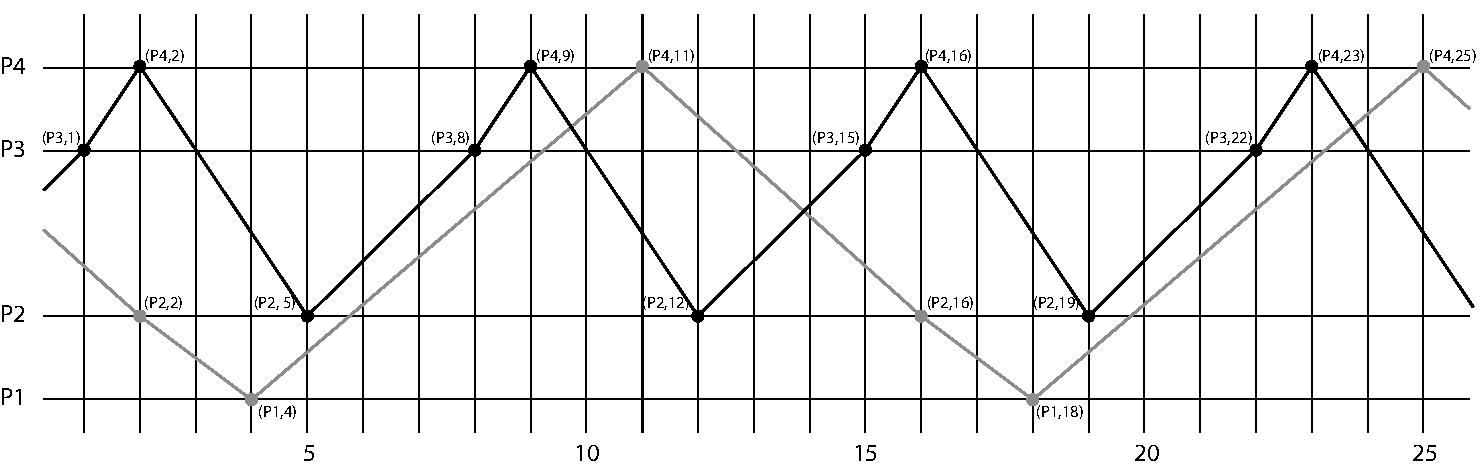
\includegraphics[scale = 0.54]{figures/Network2ServicesB.pdf}
	\caption{Small network of port calls with two services.}
	\label{fig:Network2ServicesB}
	\end{center}
\end{figure}

For this experiment, we use the same type of vessel for both vessels. The used vessel is very large, and this size does not fit well with a small network like the one considered for this experiment. The small number of ports visited by each vessel means that if the vessel is filled adequately then an improbable large amount of time is needed at each port to load and discharge cargo. 
To achieve a more realistic residual capacity, some of the ROB cargo is assumed to be destined to a time and place after the last date and it is not allowed to be left at yard to be picked up later. However, the cargo is allowed to be rearranged.

The vessel is divided into 6 sections. 
\red{Something short about which type of cargo etc? well, I guess also something about the yield (which is otherwise only explained later (?))}
The appendix contains tables showing the content of the vessel (divided into sections) as well as other key values for each of the sailing edges and each of the port calls.

Table~\ref{tab:ObjSmall} shows the objective value (the profit) when considering this network. As in the previous section we have added constraint groups one by one to see the impact of these. The abbreviations in the table is as follows: C: capacity constraints (\eqref{cap20}-\eqref{capDisp}), H: hydrostatic constraints (\eqref{defResF}-\eqref{draftLimits}), GML: GM limits (\eqref{defGM}-\eqref{minGM}), L: lashing constraints (\eqref{convexGM1}-\eqref{positiveLambdas}), O: Overstowage constraint (\eqref{overst}), MM: max moves constraints (\eqref{defMoves}-\eqref{maxPs}), and LC: long crane constraints (\eqref{longCrane}-\eqref{longCrane1Bay}). All experiments include the network flow constraint (\eqref{OnOff}-\eqref{sinks}).

\begin{table}[width=.9\linewidth,cols=2,pos=htbp]
\caption{Profit for small network with various constraints included}\label{tab:ObjSmall}
\begin{tabular*}{\tblwidth}{@{} LR @{}}
\toprule
						&Profit	(M\$)\\	
\midrule
Simple					&42.94\\	
\midrule                   
C						&30.46\\
C+H						&30.46\\
C+H+GML					&30.15\\
C+H+GML+L	(full $\mi{SCM}^\ttt{v}$)	
						&29.99\\
C+H+GML+L+O				&29.94\\	
C+H+GML+L+O+MM 			&20.75\\
C+H+GML+L+O+MM+LC (full $\mi{SCM}^\ttt{v}$ and full $\mi{SCM}^\ttt{t}$)
						&20.75\\
\bottomrule
\end{tabular*}
\end{table}

\red{Explanation of the results in the table}
%%%%%%%%%%%%%%%%%%%%%%%%%%%%%%%%%%%%%%%%%%%%%%%%%%%%%%%%%%%%%%%%%%
\subsection{Scaling results - Full-scale network}
\begin{figure}[pos=htbp]
	\centering
		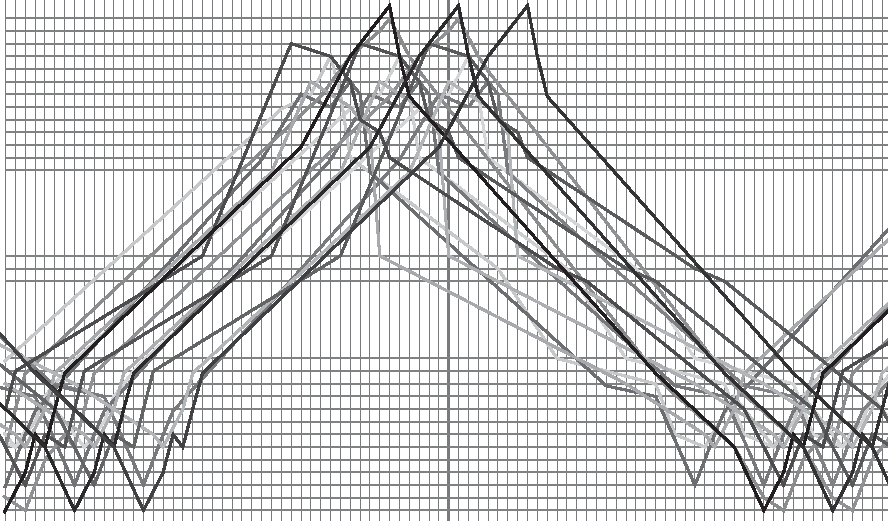
\includegraphics{figures/fewerBW.pdf}
	\caption{Vessels transporting cargo in a network from Asia to Europe within a set period of time.}
	\label{fig:full}
\end{figure}

\noindent To test our model on a full-scale network, we first consider a network of 6 different services, $R_1$ to $R_6$, that are repeated each week, resulting in a network of 67 vessels. The services connect two regions, Asia and Europe, and we are interested in maximizing the flow of cargo from one region to the other in a period of 45 days, which in the considered network is approximately the time it takes for any vessel to get from the first port visited in a region to the first port in the other region. Therefore we restrict our attention to the vessels that in the given time frame of 45 days have port calls first in Asia and then in Europe. This results in the network of $17$ vessels that are shown in Figure~\ref{fig:full}. Each service employ 3 vessel, except for service $R_3$ which only employs 2 vessels.

Each vessel already contain cargo that partly has destinations in Asia (that has not been delivered yet), and cargo with a destination in Europe (exported at the port calls in Asia prior to the current date). In order to be able to incrementally enlarge the network, the ROB cargo was generated such that it does not require transshipment. The ROB has been generated randomly such that all possible types of containers are used, the vessel is between 65-95 \% full (w.r.t. TEU-capacity); it is at most 95\% full (w.r.t. the upper displacement limit); tanks are at most 40\% full; all of the available groups are stowed; and the cargo is placed such that at most 2 different groups are stowed in the same bay, and no two adjacent sections contain cargo to the same destination. Further, the cargo is fairly evenly distributed, such that the time it will take to discharge the containers at each destination port call is within 0.8 and 1.2 of the average time per destination to unload containers, and there is a little extra time than required to deliver the cargo (allowing for potential transshipment when more vessels are considered together). The rate is chosen dependent on the type of container (see further below).
For our experiments, we have not included any cargo at the yards (this can just as well be added as required export cargo at the corresponding port call).

At each port call, we have generated a list of container groups together with a minimum and a maximum value for these (a load list). All other container groups cannot be exported at the port call. For each port call the list contains between 7 and 10 different container groups with a destination port chosen randomly between the ports on the vessel's journey in the opposite region than the port call. The deadline includes 15\% more days than what is required to reach the destination port. The length, weight class and reefer property is randomly chosen. The rate is again chosen dependent on type (see further below).  
Each container group is given a maximal export value of 4000 and a lower bound to emulate that a given cargo mix is required to be exported at the port call. The minimal values are found by finding a feasible (optimal) solution to a problem, where the export at each port is fairly evenly distributed, while the distribution of the containers of different container groups are randomly chosen. 

Move costs have been chosen depending on the length and reefer-property of the container group. This gives 4 different rates, but besides these, we also consider a fifth rate for empty (non-reefer) 40' containers (which are recognized on its weight (5t) as well). %\red{[Note to self: jeg har maaske ogsaa 40' 5t reefers, der anses som tomme]}
The rates are given below and indicates what is earned per delivered container before move costs are included. %: A 20' reefer gives 1100\$, a 20' non-reefer gives 500\$, a 40' (non-empty) reefer gives 1700\$, a 40' (non-empty) non-reefer gives 800\$, while an empty 40' container (weight of 5t) gives 200\$. 

\begin{center}
\begin{tabular}{r|rrr}
		&\mult{2}{c}{Non-empty}&Empty\\
		&Reefer	&Non-reefer	\\
\hline
20'	& 1100\$&500\$			\\
40'	& 1700\$&800\$			& 200\$
\end{tabular}
\end{center}

The move cost of a container is set to 100\$, so you earn 200\$ less per container than the rate given above, and each unnecessary move (for a transshipment) costs an additional 100\$. The tank cost is set generally to 5\$ per ton per day sailing, and the yard cost is set to 5\$ per day per reefer container and 1\$ per container per day for non-reefers.

The number of cranes available at the port calls are between 5 and 9 (5 for services $R_2$ and $R_6$, 7 for $R_1$, and 9 for $R_3$, $R_4$, and $R_5$) for all port calls on the services, and the time wondow is 18 hours for all port calls. This is chosen such that there is enough time at each port to have the vessels ``reasonable filled''.
\\\\
For our experiments, we first considered a case where only the three vessels employed in service $R_1$ are included. Then we have made an experiment where only the six vessel in $R_1$ and $R_2$ are considered, and so on. For each of these included set of services we have divided the vessel into 4, 8, 14, 20, and 26 sections, respectively, and repeated the experiments. The sections were made such that for a division of the vessel into more sections, each section remains the same or is divided into two or more sections. We also made an experiment, where we only included the ``simple'' model (referred to previously) - in the table this is referred to as a result with 1 section, though this is not completely accurate. 

Table~\ref{tab:BigObj} shows the found objective values for each of these experiments. Besides the objective values, the table also shows the {difference (overestimation) in percentage of the lower objective value to the higher objective value}. As the results show, the overestimation of the simple model compared to the most accurate model ($|S|=26$) is approximately 20\% except in the case where we only consider the first service. \red{Maybe the reason is that there is not that much chance/option/possibility for taking advantage of the whole network to rearrange cargo}. In this case, the overestimation is only app. 9\%. The results also show, that although more accuracy is gained from a higher number of sections, the largest difference lies  (maybe not surprisingly) in dividing the vessel at all, i.e. between using the simple model and dividing the vessel into 4 sections.  

\begin{table}[width=.9\linewidth,cols=8,pos=htbp]
\caption{Objective values ($10^7$\$)}\label{tab:BigObj}
\begin{tabular*}{\tblwidth}{@{} LR *{6}{R} @{}}
\toprule
&						 			  &  \multicolumn{6}{c}{Included services}\\		
\cmidrule{3-8}
&									  & $R_1$		& $R_1$ to $R_2$&$R_1$ to $R_3$&$R_1$ to $R_4$&$R_1$ to $R_5$&$R_1$ to $R_6$\\		
\midrule
\parbox[t]{2mm}{\multirow{6}{*}{\rotatebox[origin=c]{90}{Sections}}}
&1									& 2.2110	& 5.5289	&   7.6939	& 11.709	&	16.310	&	19.869\\
&4									& 2.1030	& 4.6781	&   6.6464	& 10.234	&	13.981	&	16.892\\
&8									& 2.0742	& 4.6499	&   6.6103	& 10.190	&	13.923	&	16.830\\
&14									& 2.0588	& 4.6223	&   6.5681	& 10.138	&	13.863	&	16.762\\
&20									& 2.0515	& 4.5872	&   6.5090	& 10.063	&	13.767	&	16.653\\
&26									& 2.0249	& 4.4985	&   6.3882	&  9.959	&	13.651	&	16.523\\
\midrule                                   
\parbox[t]{2mm}{\multirow{3}{*}{\rotatebox[origin=c]{90}{Dif.(\%)}}}
&1 to 4		&   5.14	&  18.19	&    15.76	&  14.41	&	 16.66	&	 17.62\\	
&4 to 26	&   3.85	&   3.99	&     4.04	&   2.76	&	  2.42	&	  2.23\\
&1 to 26	&   9.19	&  22.90	&    20.44	&  17.57	&	 19.48	&	 20.25\\
\bottomrule
\end{tabular*}
\end{table}

Table~\ref{tab:BigSize2} and Table~\ref{tab:BigSize} show the size of the underlying time-space graph (as in Figure~\ref{fig:timespace}) and the size of the produced LPs (after cplex' preprocessing), and Table~\ref{tab:BigTime} shows the solution time (in seconds, ticks and iterations). Each experiment is only solved once. As expected, the size and time to solve increases the more services are added, and the more horizontal sections are considered. The only exceptions are for one service, where the time falls for 26 section compared to 20 sections, and the number of iterations with 3 services that falls from 20 to 26 sections. The important thing to notice here, however, is that even the full network with most accuracy finishes within reasonable time (23 minutes). Using only 4 sections (for the full network) finishes within 7 minutes, which still saves us an overestimation of 17\%.

\begin{table}[width=.9\linewidth,cols=4,pos=htbp]
\caption{Size of time-space networks.}\label{tab:BigSize2}
\begin{tabular*}{\tblwidth}{@{} LRRR @{} }
\toprule
Services&Nodes&Edges&Groups\\
\midrule
        $R_1$ &  59 &  62 & 251\\
$R_1$ - $R_2$ & 110 & 116 & 516\\
$R_1$ - $R_3$ & 147 & 155 & 685\\
$R_1$ - $R_4$ & 191 & 202 & 919\\
$R_1$ - $R_5$ & 242 & 252 &1177\\
$R_1$ - $R_6$ & 296 & 313 &1409\\
\bottomrule
\end{tabular*}
\end{table}

\begin{table}[width=.9\linewidth,cols=11,pos=htbp]
\caption{Size (rows/column/non-zeros) of preprocessed LPs.}\label{tab:BigSize}
\begin{tabular*}{\tblwidth}{@{} RR *{2}{R@{\;/\hspace{-2mm}}R@{\;/\hspace{-2mm}}R@{$\quad$}} *{1}{R@{\;/\hspace{-2mm}}R@{\;/\hspace{-2mm}}R} @{}}
\toprule
&		&\mult{9}{c}{Included services}\\
\cmidrule{3-11}
&		&	\mult{3}{c}{$R_1$}&\mult{3}{c}{$R_1$ to $R_2$}&\mult{3}{c}{$R_1$ to $R_3$}\\	
\midrule
\parbox[t]{2mm}{\multirow{6}{*}{\rotatebox[origin=c]{90}{Sections}}}
&1		&   1588&    2224&   13969	&   4366&    6480&   37767	&   8554&   12700&   70157	\\ 
&4		&  31935&   42478&  250599	&  77510&  107289&  647873	& 128863&  183300& 1110277	\\ 
&8		&  56834&   77178&  455850	& 137554&  194588& 1174943	& 229449&  333676& 2021683	\\ 
&14		&  86505&  118873&  708442	& 209417&  299866& 1826194	& 348880&  513184& 3134208	\\ 
&20		& 117221&  161085&  957727	& 282894&  405345& 2458949	& 472519&  696228& 4233583	\\ 
&26		& 139301&  191323& 1133259	& 335578&  480726& 2900880	& 561841&  828201& 5007594	\\ 
&\mult{6}{r}{}\\
&			&\mult{3}{c}{$R_1$ to $R_4$}&\mult{3}{c}{$R_1$ to $R_5$}&\mult{3}{c}{$R_1$ to $R_6$}\\
\cmidrule{3-11}
\parbox[t]{2mm}{\multirow{6}{*}{\rotatebox[origin=c]{90}{Sections}}}
&1		&  12525&   18709&   98262	&  21601&   32588&  164935	&  29152&   44118&  216482\\
&4		& 169622&  244564& 1489524	& 258157&  378523& 2333959	& 330756&  487704& 3009184\\
&8		& 301941&  444977& 2711406	& 458443&  686773& 4240073	& 587928&  885302& 5469498\\
&14		& 459201&  684373& 4203846	& 697520& 1056348& 6573040	& 894364& 1361065& 8475430\\
&20		& 621669&  928150& 5676748	& 941161& 1428208& 8850565	&1208029& 1842194&11422129\\
&26		& 739023& 1103928& 6713520	&1115569& 1693872&10437186	&1433394& 2187254&13481176\\
\bottomrule
\end{tabular*}
\end{table}

\begin{table}[width=.9\linewidth,cols=11,pos=htbp]
\caption{Time (seconds (iterations/ticks))}\label{tab:BigTime}
\begin{tabular*}{\tblwidth}{@{} RR *{2}{R@{\;(\hspace{-5mm}}R@{\;/\hspace{-5mm}}R@{\;)$\quad$}} *{1}{R@{\;(\hspace{-5mm}}R@{\;/\hspace{-5mm}}R@{\;)}} @{}}
\toprule
&			&\mult{9}{c}{Included services}\\
\cmidrule{3-11}
&			&\mult{3}{c}{$R_1$}&\mult{3}{c}{$R_1$ to $R_2$}&\mult{3}{c}{$R_1$ to $R_3$}\\	
\midrule
\parbox[t]{2mm}{\multirow{6}{*}{\rotatebox[origin=c]{90}{Sections}}}
&1	&	 0.30&  26&      46.87&	   0.33&  25&     148.49&	   3.67&  30&     297.20\\	
&4	&  	 5.80&  55&    4193.96&	  22.25&  66&   20882.71&	  58.48&  53&   56171.97\\	
&8	&	12.11&  72&    9098.21&	  40.92&  91&   38334.37&	 105.41&  79&   99126.82\\	
&14	&	26.02&  80&   19288.74&	  60.48&  99&   57916.81&	 144.00&  84&  134143.64\\	
&20	&	38.77&  86&   27304.82&	 112.59& 121&   96272.11&	 225.45& 101&  206696.07\\	
&26	&	31.66&  92&   25940.18&	 141.84& 133&  120508.32&	 294.02& 116&  269259.79\\	
\mult{6}{r}{}\\
&			&\mult{3}{c}{$R_1$ to $R_4$}&\mult{3}{c}{$R_1$ to $R_5$}&\mult{3}{c}{$R_1$ to $R_6$}\\
\cmidrule{3-11}
\parbox[t]{2mm}{\multirow{6}{*}{\rotatebox[origin=c]{90}{Sections}}}
&1	&    0.94&  33&     483.96&	   1.83&  40&     906.31&	   6.13&  47&    1408.14\\
&4	&   85.20&  65&   89606.75&	 243.64&  61&  241979.21&	 374.94&  61&  382790.35\\
&8	&  152.34&  85&  140197.50&	 381.48&  80&  371760.54&	 536.31&  79&  538352.53\\
&14	&  235.17&  92&  219897.94&	 544.59&  91&  546520.75&	 813.78&  96&  822709.17\\
&20	&  335.39& 109&  299161.00&	 753.38& 112&  730976.96&	1164.17& 112& 1173676.98\\
&26	&  394.14& 108&  353180.07&	 890.95& 122&  833032.20&	1346.00& 114& 1328244.24\\
\bottomrule
\end{tabular*}
\end{table}

\red{To obtain these values, we have used cplex' standard Barrier method without crossover %[barrier algorithm choice: 3], barrier crossover choice = -1, 
with a convergence tolerance of 0.0001 and available working memory of 30 GB.} % and a time limit of 1800 seconds. - that was never met}
%http://www.maximalsoftware.com/solvopt/optCpxBarrier.html: The Convergence Tolerance sets the tolerance on complementarity for convergence. The barrier algorithm will terminate with an optimal solution if the relative complementarity is smaller than this value. The default value is le-8.
%http://www-eio.upc.edu/lceio/manuals/cplex75/doc/usermanccpp/html/solveLPS28.html: In the Interactive Optimizer, options to the baropt command control whether the ILOG CPLEX Barrier Optimizer stops with a nonbasic solution or crosses over to a simplex optimizer to generate a basic solution. Table 4.8 summarizes those options to the baropt command in the Interactive Optimizer.
%https://www.tu-chemnitz.de/mathematik/discrete/manuals/cplex/doc/refman/html/appendixA4.html


\subsubsection{Generation of data} 
\red{This section is not that important. Maybe summarized within the previous section.} 
The ROB of each vessel is generated as follows. We use all 16 container types. These are divided into a set that will get a destination in the current region and a set that will get a destination in the other region. The types are randomly distributed in the two sets such that the percentage of types with a destination in the other region corresponds to the percentage of port calls in this region that was visited before the current date. Types predestined to a port in this region then gets assigned a destination among the ports from the journey from the current date until it is no more in this region, minus ports that were already visited in the region before the current date. Likewise, the other types gets assigned a destination in the other region. (Btw., the ports are cycled through (in a random order, and then we potentially start over, so the ports are not randomly distributed). For a deadline, we find the least time it takes to get to the port, and then we add 6\% (and find the port call closets, but earlier).
Given the available container groups, we find a feasible integer solution (by optimizing a dummy objective) to a model with the sailing constraints (\ref{}-\ref{}), where we further require that the vessel is between 65-95 \% full (w.r.t. TEU-capacity); it is at most 95\% full (w.r.t. displacement limit); tanks are at most 40\% full; all of the available groups are stowed (there are more than 40 of each group); and the cargo is placed such that at most 2 different groups are stowed in the same bay, and no two horizontal sections contain cargo to the same destination. Further, the cargo is fairly evenly distributed, such that the time it will take to unload the containers at each destination port call is within 0.8 and 1.2 of the average time per destination to unload containers.

For a vessel, the loadlists is generated as follows: For each port call, we randomly choose between 7 and 10 container groups. Each group's destination port is chosen randomly between the ports in the opposite region that is on the vessel's journey (in order to be able to incrementally add services), and for the deadline we add 15\% more days than what is required to reach the destination port and then we find the port call (in the whole network) that is closets but earlier than that. The length, weight class and reefer property is randomly chosen. The rate is chosen dependent on the length, weight and reefer-property. (Implementation-wise, we therefore also do not have a deadline in the set of dates, but a date, and then we find the closest to).
For each vessel, the lower bound for export is generated as follows: We make the model described previously, where we add the following further constraints. We ensure that there is an fairly even distribution of exported containers among the port calls on the journey by requiring that the number of exports at a port call is within 0.5 and 2 of the average exports per port call. Then, for each port call on the vessel's journey, we divide the container groups into reefers and non-reefers. For each of these two sets, we assign a random percentage to each container group so that the percentages adds up to 1. (In reality, each group gets a random number $r_g$ number between 1 and 51, and the assigned percentage is then $\frac{n_g}{\sum_{g'}n_{g'}}$). We then require that the number of containers of that group constitutes that percentage of containers being loaded (from that set). Then we require (if there is any reefers in the loadlist) that 10 percent of the containers being exported at the port call are reefers. We then maximize the total export (on the one-service network) with 26 parts and all constraints and let the results (rounded down) for each port call and each group be the lower bound.   

 

\section{Conclusion}
\section*{Aknowledgments}

\appendix
\section{Appendix}
This appendix shows an example of which information can be extracted from our model. 
We consider the network of port calls made by two vessels that is shown in Figure~\ref{fig:Network2ServicesB}. 
  
The considered container groups are listed in Table~\ref{tab:groupIDs} together with an ID (used for brevity in tables to follow). The container groups are listed with a length, a weight class, its reefer property, its destination POD, the deadline (date), and a rate. Notice that not all container types (combinations of length, weight, and reefer-property) are present. As explained in Section~\ref{sec:smallNetwork}, some container groups are to be delievered later than the last day in the network, which is noted as ``later'' in this table. 

\begin{table}[width=.9\linewidth,cols=23,pos=h]
\caption{ID of used container groups.}\label{tab:groupIDs}
\begin{scriptsize}
\begin{tabular*}{\tblwidth}{@{} *{2}{ R@{\hspace{2mm}} *{5}{R@{\hskip3pt}}RC@{\hspace{7mm}}} R@{\hspace {2mm}} *{5}{R@{\hskip3pt}}R @{}}
\toprule
	ID&\mult{6}{l}{Container group}&&ID&\mult{6}{l}{Container group}&&ID&\mult{6}{l}{Container group}\\
	\cmidrule{1-7}							 \cmidrule{9-15}						\cmidrule{17-23}
   0&(20,& 5,&NR),&(P3,& 1),& 500&	& 	    24&(20,& 5,&NR),&(P3,& 8),& 500&  &     48&(20,& 5,&NR),&(P1,&18),& 500\\       
   1&(40,& 5,&NR),&(P3,& 1),& 200&  &       25&(20,&13,&NR),&(P3,& 8),& 500&  &     49&(20,&13,&NR),&(P1,&18),& 500\\  
   2&(20,& 5,&NR),&(P2,& 2),& 500&  &       26&(20,&19,& R),&(P3,& 8),&1100&  &     50&(20,&19,& R),&(P1,&18),&1100\\
   3&(20,&13,&NR),&(P2,& 2),& 500&  &       27&(40,& 5,&NR),&(P3,& 8),& 200&  &     51&(40,& 5,&NR),&(P1,&18),& 200\\
   4&(40,& 5,&NR),&(P2,& 2),& 200&  &       28&(40,&13,& R),&(P3,& 8),&1700&  &     52&(40,&13,& R),&(P1,&18),&1700\\
   5&(40,&26,&NR),&(P2,& 2),& 800&  &       29&(40,&26,&NR),&(P3,& 8),& 800&  &     53&(40,&26,&NR),&(P1,&18),& 800\\
   6&(20,& 5,&NR),&(P4,& 2),& 500&  &       30&(20,& 5,&NR),&(P4,&11),& 500&  &     54&(20,& 5,&NR),&(P2,&19),& 500\\
   7&(20,&13,&NR),&(P4,& 2),& 500&  &       31&(20,&13,&NR),&(P4,&11),& 500&  &     55&(20,&13,&NR),&(P2,&19),& 500\\
   8&(20,&19,& R),&(P4,& 2),&1100&  &       32&(20,&19,& R),&(P4,&11),&1100&  &     56&(20,&19,& R),&(P2,&19),&1100\\
   9&(40,& 5,&NR),&(P4,& 2),& 200&  &       33&(40,& 5,&NR),&(P4,&11),& 200&  &     57&(40,& 5,&NR),&(P2,&19),& 200\\
  10&(40,&13,& R),&(P4,& 2),&1700&  &       34&(40,&13,& R),&(P4,&11),&1700&  &     58&(40,&13,& R),&(P2,&19),&1700\\
  11&(40,&26,&NR),&(P4,& 2),&1700&  &       35&(40,&26,&NR),&(P4,&11),& 800&  &     59&(40,&26,&NR),&(P2,&19),& 800\\
  12&(20,& 5,&NR),&(P1,& 4),& 500&  &       36&(20,& 5,&NR),&(P2,&12),& 500&  &     60&(20,& 5,&NR),&(P3,&22),& 500\\
  13&(20,&13,&NR),&(P1,& 4),& 500&  &       37&(20,&13,&NR),&(P2,&12),& 500&  &     61&(20,&13,&NR),&(P3,&22),& 500\\
  14&(20,&19,& R),&(P1,& 4),&1100&  &       38&(20,&19,& R),&(P2,&12),&1100&  &     62&(20,&19,& R),&(P3,&22),&1100\\
  15&(40,& 5,&NR),&(P1,& 4),& 200&  &       39&(40,& 5,&NR),&(P2,&12),& 200&  &     63&(40,& 5,&NR),&(P3,&22),& 200\\
  16&(40,&13,& R),&(P1,& 4),&1700&  &       40&(40,&13,& R),&(P2,&12),&1700&  &     64&(40,&13,& R),&(P3,&22),&1700\\
  17&(40,&26,&NR),&(P1,& 4),& 800&  &       41&(40,&26,&NR),&(P2,&12),& 800&  &     65&(40,&26,&NR),&(P3,&22),& 800\\
  18&(20,& 5,&NR),&(P2,& 5),& 500&  &       42&(20,& 5,&NR),&(P3,&15),& 500&  &     66&(20,& 5,&NR),&\mult{2}{l}{later,}& 500\\
  19&(20,&13,&NR),&(P2,& 5),& 500&  &       43&(20,&13,&NR),&(P3,&15),& 500&  &     67&(20,&19,& R),&\mult{2}{l}{later,}&1100\\
  20&(20,&19,& R),&(P2,& 5),&1100&  &       44&(20,&19,& R),&(P3,&15),&1100&  &     68&(20,& 5,&NR),&\mult{2}{l}{later,}& 500\\
  21&(40,& 5,&NR),&(P2,& 5),& 200&  &       45&(40,& 5,&NR),&(P3,&15),& 200&  &     69&(20,&13,&NR),&\mult{2}{l}{later,}& 500\\
  22&(40,&13,& R),&(P2,& 5),&1700&  &       46&(40,&13,& R),&(P3,&15),&1700&  &     70&(40,&13,& R),&\mult{2}{l}{later,}&1700\\
  23&(40,&26,&NR),&(P2,& 5),& 800&  &       47&(40,&26,&NR),&(P3,&15),& 800&  &     71&(40,&26,&NR),&\mult{2}{l}{later,}& 800\\
  \bottomrule
\end{tabular*}
\end{scriptsize}
\end{table}

Table~\ref{tab:loadLists} summarizes the groups that are available to import at each port call. Each group has a maximal import of 1000, and the groups that are underlined have a minimal/required import of 100 containers.
  
\begin{table}[width=.9\linewidth,cols=2,pos=h]
\begin{scriptsize}
\begin{tabular*}{\tblwidth}{@{} RL @{}}
\toprule
Port call 			   & Groups possible to load\\
\midrule
	(P2,\phantom{ 1}2) & \{12, 13, 14, 15, 16, 17, \ul{30}, 31, 32, 33, \ul{34}, \ul{35}, 42, 43, 44, 45, 46, 47\}\\
	(P1,\phantom{ 1}4) & \{30, 31, \ul{32}, \ul{33}, 34, 35, 54, 55, \ul{56}, 57, 58, 59, 60, \ul{61}, \ul{62}, 63, 64, 65\}\\
	(P4,		   11) & \{47, 48, 49, \ul{50}, 51, 52, \ul{53}, 54, 55, \ul{56}, 57, 58, 59, 60, 61, 62, \ul{63}, 64\}\\
	(P3,\phantom{ 1}1) & \{\ul{6}, 7, 8, 9, \ul{10}, 11, 18, \ul{19}, 20, 21, \ul{22}, 23, 30, 31, \ul{32}, \ul{33}, 34, 35, 48, 49, 50, \ul{51}, 52, 53\}\\
	(P4,\phantom{ 1}2) & \{18, 19, 20, 21, \ul{22}, \ul{23}, 24, \ul{25}, 26, 27, 28, 29, 36, 37, \ul{38}, 39, \ul{40}, 41, \ul{48}, 49, 50, 51, 52, \ul{53}\}\\
	(P2,\phantom{ 1}5) & \{\ul{24}, 25, 26, \ul{27}, \ul{28}, 29, 30, 31, 32, 33, 34, \ul{35}, 48, \ul{49}, 50, 51, \ul{52}, 53\}\\
	(P3,\phantom{ 1}8) & \{30, 31, \ul{32}, 33, \ul{34}, 35, 48, 49, 50, 51, 52, 53, 54, 55, 56, \ul{57}, 58, \ul{59}\}\\
	(P4,\phantom{ 1}9) & \{\ul{42}, 43, 44, 45, 46, 47, 48, 49, 50, \ul{51}, 52, 53, 54, 55, 56, \ul{57}, 58, \ul{59}\}\\
\bottomrule
\end{tabular*}
\caption{Load lists. Underlined group IDs have a minimum import of 100 containers.}\label{tab:loadLists}
\end{scriptsize}
\end{table}

The vessel is divided into 6 sections. 
Table~\ref{tab:smallNetLegs} below shows what is on the two vessels ($V_1$ and $V_2$) on their journeys (within the horizon). For each leg, the content of the 6 sections, on deck (o) and below deck (b), is given in terms of the number of containers of each type of container that is on board the vessel. Likewise, the content of the tanks is given, as well as the total TEU-usage, the total displacement, trim, draft, and the GM. The legs indicated with no starting port call display the ROB on board the vessels when they enter the network.

\addtolength{\tabcolsep}{-5pt}   
\begin{table}[width=0.9\linewidth,cols=19,pos=h]
\caption{Key numbers for sailing edges.\label{tab:smallNetLegs}}
\begin{scriptsize}
\begin{tabular*}{\tblwidth}{@{} r@{\hspace{2mm}}r@{\hspace{2mm}} R@{\hspace{-2mm}}RC R@{\hspace{-2mm}}RC R@{\hspace{-2mm}}RC R@{\hspace{-2mm}}RC R@{\hspace{-2mm}}RC R@{\hspace{-2mm}}R @{}}
\toprule
\mult{4}{l}{Leg $\quad\rightarrow (P2,2)\;(V_1)$}\\
	&		 &\mult{17}{c}{Sections}\\
\cmidrule{3-19}
	&		 & \mult{2}{c}{1} &&	 \mult{2}{c}{2}&&	  \mult{2}{c}{3}&&\mult{2}{c}{4}	 &&		\mult{2}{c}{5}&& \mult{2}{c}{6}\\
\cmidrule{3-4}\cmidrule{6-7}\cmidrule{9-10}\cmidrule{12-13}\cmidrule{15-16}\cmidrule{18-19}
ID	&Total   &\mult{1}{c}{o}&\mult{1}{c}{b}&&\mult{1}{c}{o}&\mult{1}{c}{b}&&\mult{1}{c}{o}&\mult{1}{c}{b}&&\mult{1}{c}{o}&\mult{1}{c}{b}&&\mult{1}{c}{o}&\mult{1}{c}{b}&&\mult{1}{c}{o}&\mult{1}{c}{b}\\
\midrule
 2	&  518.0 &  85.0&        -&&     42.0&        -&&     35.0&        -&&        -&        -&&     70.0&        -&&    110.0&    176.0\\         
 3	&  821.0 &     -&     88.0&&        -&        -&&    170.0&    116.0&&        -&        -&&    131.0&    241.0&&     31.0&     44.0\\         
 4	&   59.0 &     -&     56.0&&        -&        -&&        -&        -&&        -&        -&&        -&        -&&      3.0&        -\\         
 5	&  618.0 &     -&        -&&        -&        -&&        -&    146.0&&        -&      1.0&&    175.0&        -&&    279.0&     17.0\\         
12	&  801.0 &   1.0&        -&&    155.0&        -&&        -&        -&&    445.0&        -&&     70.0&        -&&    130.0&        -\\         
13	& 1381.0 & 283.0&        -&&        -&    420.0&&    232.0&        -&&    120.0&        -&&    295.0&        -&&     31.0&        -\\         
15	&  367.0 &     -&        -&&        -&     40.0&&     23.0&        -&&    190.0&     79.0&&      8.0&        -&&        -&     27.0\\         
16	&  416.0 &     -&        -&&    102.0&     90.0&&    174.0&     50.0&&        -&        -&&        -&        -&&        -&        -\\         
17	&  593.0 &  80.0&        -&&    122.0&        -&&     53.0&     60.0&&      3.0&    180.0&&     95.0&        -&&        -&        -\\         
68	& 1038.0 &  65.0&     65.0&&    150.0&    160.0&&     30.0&        -&&    280.0&        -&&        -&    188.0&&    100.0&        -\\         
69	&\;1029.0 &100.0&        -&&    150.0&        -&&    237.0&        -&&     80.0&        -&&        -&    240.0&&        -&    222.0\\         
70	&  362.0 &     -&        -&&        -&    120.0&&        -&    242.0&&        -&        -&&        -&        -&&        -&        -\\         
71	&  882.0 &     -&        -&&        -&        -&&        -&    246.0&&        -&    541.0&&        -&        -&&     95.0&        -\\   
\midrule
\mult{2}{l}{Ballast}
		&\mult{2}{r}{     -}&&\mult{2}{r}{     -}&&\mult{2}{r}{11381.9}&&\mult{2}{r}{8658.2}&&\mult{2}{r}{    -}&&\mult{2}{r}{    -}\\%&    TEU: 12182.0\\
\mult{2}{l}{Sf/Bm}
		&-4916/	  &   191411&&     1805/&   389471&&    -6314/&   629236&&      482/&   866123&&    14188/&   437835&& \phantom{14188/}&\phantom{437835}\\
\midrule
	&		 &Trim =& - 2.16&& Draft =& 15.07&&GM = &0.75&&TEU = &12182.0&&Disp. = &218788\\
\midrule
\mult{2}{c}{}\\
\mult{4}{l}{Leg $(P2,2)\rightarrow (P1,4)\;(V_1)$}\\
\midrule
   12&  801.0&   1.0&        -&&    155.0&        -&&        -&       -&&   445.0&        -&&    70.0&        -&&   130.0&        -\\
   13& 1381.0& 283.0&        -&&        -&    420.0&&    232.0&       -&&   120.0&        -&&   295.0&        -&&    31.0&        -\\
   14&  168.0&     -&        -&&        -&        -&&        -&       -&&       -&    168.0&&       -&        -&&       -&        -\\
   15&  367.0&     -&        -&&        -&     40.0&&     48.7&       -&&   190.0&        -&&     8.0&     53.3&&       -&     27.0\\
   16&  516.0&     -&        -&&    106.0&     90.0&&    186.0&    50.0&&    64.0&     20.0&&       -&        -&&       -&        -\\
   17&  593.0&  26.4&        -&&    122.0&        -&&     53.0&   102.9&&    13.7&    180.0&&    95.0&        -&&       -&        -\\
   30&  560.8&     -&        -&&    136.6&        -&&    109.3&   315.0&&       -&        -&&       -&        -&&       -&        -\\
   31&  924.9&     -&        -&&        -&        -&&        -&       -&&       -&        -&&   146.4&    778.5&&       -&        -\\
   32&  100.0&     -&        -&&        -&        -&&        -&       -&&       -&    100.0&&       -&        -&&       -&        -\\
   35&  100.0&     -&        -&&        -&        -&&        -&       -&&       -&        -&&   100.0&        -&&       -&        -\\
   68& 1038.0&  65.0&     65.0&&    150.0&    160.0&&     74.5&       -&&   235.5&        -&&       -&    188.0&&   100.0&        -\\
   69& 1029.0& 100.0&        -&&    150.0&        -&&    237.0&       -&&    80.0&        -&&       -&    240.0&&       -&    222.0\\
   70&  362.0&     -&        -&&        -&    120.0&&        -&   242.0&&       -&        -&&       -&        -&&       -&        -\\
   71&  882.0&     -&        -&&        -&        -&&        -&   249.6&&       -&    467.0&&    70.4&        -&&    95.0&        -\\
\midrule
\mult{2}{l}{Ballast}   
		 &\mult{2}{r}{    -}&&\mult{2}{r}{     -}&&\mult{2}{r}{13073.2}&&\mult{2}{r}{8658.2}&&\mult{2}{r}{4114.3}&&\mult{2}{r}{   -}\\
\mult{2}{l}{Sf/Bm}&
         -1924/&    74929&&      287/&   123187&&    -2322/&   183297&&      729/&   248002&&     3775/&   116498&& \phantom{3775/}&\phantom{116498}\\
\midrule
\end{tabular*}
\begin{tabular*}{\tblwidth}{@{} RRRRR @{}}
Trim = -1.50& Draft = 15.37 & GM = 2.85 & Displacement = 218788.00 & TEU = 11642.8\\
\bottomrule
\end{tabular*}
\end{scriptsize}
\end{table}

%%%%%%%%%%%%%%%%%
%\mult{2}{c}{}\\%	------
%\multicolumn{7}{l}{Leg $(P1,4)\rightarrow (P4,11)\;(V_1)$}\vspace{1mm}\\
%\hline
%  30&        -&        -&    136.6&        -&    109.3&    315.0&        -&        -&        -&        -&        -&        -&           560.8\\
%  31&        -&        -&        -&        -&        -&        -&        -&        -&    146.4&    778.5&        -&        -&           924.9\\
%  32&        -&        -&    212.0&     80.0&    272.0&    100.0&    128.0&    308.0&        -&        -&        -&        -&          1100.0\\
%  33&     50.7&     49.1&        -&      0.2&        -&        -&        -&        -&        -&        -&        -&        -&           100.0\\
%  35&        -&        -&        -&        -&        -&        -&        -&        -&    100.0&        -&        -&        -&           100.0\\
%  56&        -&        -&        -&    100.0&        -&        -&        -&        -&        -&        -&        -&        -&           100.0\\
%  60&    569.2&        -&        -&        -&        -&    156.8&        -&        -&    151.0&        -&        -&        -&           876.9\\
%  61&        -&    249.5&        -&        -&        -&        -&        -&        -&    399.2&    185.5&    165.8&        -&          1000.0\\
%  62&        -&        -&        -&        -&    100.0&        -&        -&        -&        -&        -&        -&        -&           100.0\\
%  68&     65.0&     65.0&    150.0&    160.0&     74.5&        -&    235.5&        -&        -&    188.0&    100.0&        -&          1038.0\\
%  69&    100.0&        -&    150.0&        -&    237.0&        -&     80.0&        -&        -&    240.0&        -&    222.0&          1029.0\\
%  70&        -&        -&        -&    120.0&        -&    242.0&        -&        -&        -&        -&        -&        -&           362.0\\
%  71&        -&        -&        -&        -&        -&    249.6&        -&    467.0&     70.4&        -&     95.0&        -&           882.0\\
%\hline
%\mult{1}{r|}{Ballast}   
%		&\mult{2}{r}{     -}&\mult{2}{r}{     -}&\mult{2}{r}{     -}&\mult{2}{r}{     -}&\mult{2}{r}{     -}&\mult{2}{r|}{     -}\\
%\mult{1}{r|}{Sf/Bm}&
%				 -6755&   263014&    -5432&   622130&    -1972&   840750&     7128&   631313&     7047&   217472 \vspace{1mm}\\      
%\mult{1}{c}{}	&\mult{1}{r}{Trim}& \mult{1}{r}{0.00}& \mult{1}{r}{Draft} & \mult{1}{r}{13.79}&\mult{1}{r}{GM}&\mult{1}{r}{3.54}& \mult{2}{r}{Displacement}&\mult{2}{r}{184515.97} &\mult{1}{r}{TEU}& \mult{1}{r}{9617.7}\\
%%%%%%%%%%%%%%%%%
%\mult{2}{c}{}\\%	------
%\mult{7}{l}{Leg $\quad\rightarrow (P3,1)\;(V_2)$}\vspace{1mm}\\
%\hline
%   0&       -&        -&        -&        -&        -&    270.0&    290.0&        -&    385.0&        -&    516.0&        -&          1461.0\\
%   1&       -&        -&     56.0&     80.0&        -&        -&     17.0&        -&     55.0&        -&        -&        -&           208.0\\
%   6&       -&        -&        -&    100.0&    330.0&        -&        -&        -&    125.0&    292.0&        -&     90.0&           937.0\\
%   8&       -&        -&        -&        -&    110.0&        -&    118.0&        -&        -&        -&        -&        -&           228.0\\
%  11&   285.0&     76.0&     65.0&        -&    198.0&    235.0&    264.0&    249.0&    240.0&    266.0&    339.0&     18.0&          2235.0\\
%  32&       -&        -&    188.0&    400.0&    134.0&     10.0&        -&        -&        -&        -&        -&        -&           732.0\\
%  66&    90.0&    166.0&    190.0&    230.0&    185.0&    280.0&    240.0&   1084.0&    200.0&    558.0&        -&    274.0&          3497.0\\
%  67&       -&        -&        -&        -&        -&    540.0&        -&        -&        -&        -&        -&        -&           540.0\\
%\hline 
%\mult{1}{r|}{Ballast}   
%		&\mult{2}{r}{     -}&\mult{2}{r}{     -}&\mult{2}{r}{2579.4}&\mult{2}{r}{8658.2}&\mult{2}{r}{1490.1}&\mult{2}{r|}{     -}\\
%\mult{1}{r|}{Sf/Bm}&
%				-6526&   254105&    -3466&   548570&    -3453&   752911&     2656&   785275&    11785&   363670\vspace{1mm}\\      
%\mult{1}{c}{}	&\mult{1}{r}{Trim}& \mult{1}{r}{-2.50}& \mult{1}{r}{Draft} & \mult{1}{r}{14.21}&\mult{1}{r}{GM}&\mult{1}{r}{0.85}& \mult{2}{r}{Displacement}&\mult{2}{r}{208150.66} &\mult{1}{r}{TEU}& \mult{1}{r}{12281.0}\\
%%%%%%%%%%%%%%%%%
%\mult{2}{c}{}\\%	------
%\mult{7}{l}{Leg $(P3,1)\rightarrow (P4,2)\;(V_2)$}\vspace{1mm}\\
%\hline
%   6&       -&        -&     36.2&    100.0&    330.0&        -&        -&        -&    188.8&    292.0&        -&     90.0&          1037.0\\
%   8&       -&        -&        -&        -&     33.2&     34.0&    118.0&     42.8&        -&        -&        -&        -&           228.0\\
%  10&       -&        -&    106.0&        -&     69.4&        -&        -&        -&        -&        -&        -&        -&           175.4\\
%  11&   224.9&     76.0&     65.0&        -&    198.0&    289.1&    264.0&    249.0&    240.0&    266.0&    339.0&     24.0&          2235.0\\
%  18&       -&    102.0&    461.3&    240.9&        -&        -&        -&        -&        -&        -&    195.8&        -&          1000.0\\
%  19&       -&        -&        -&    185.1&        -&     61.8&        -&        -&        -&     10.0&        -&    304.0&           560.9\\
%  20&       -&        -&        -&     20.0&        -&        -&        -&    248.6&        -&        -&        -&        -&           268.6\\
%  22&       -&        -&        -&        -&    100.0&        -&        -&        -&        -&        -&        -&        -&           100.0\\
%  32&       -&        -&        -&    400.0&        -&     10.0&        -&        -&        -&        -&        -&        -&           410.0\\
%  33&    20.0&        -&     53.8&        -&     26.1&        -&        -&        -&        -&        -&        -&        -&           100.0\\
%  48&       -&        -&     83.3&        -&        -&        -&    322.0&        -&    227.4&        -&    367.3&        -&          1000.0\\
%  49&       -&        -&        -&        -&        -&    100.0&        -&        -&        -&        -&        -&        -&           100.0\\
%  51&   100.0&        -&        -&        -&        -&        -&        -&        -&        -&        -&        -&        -&           100.0\\
%  66&    90.0&    166.0&    249.0&    230.0&    185.0&    280.0&    240.0&    812.6&    412.4&    558.0&        -&    274.0&          3497.0\\
%  67&       -&        -&        -&        -&        -&    540.0&        -&        -&        -&        -&        -&        -&           540.0\\
%\hline 
%\mult{1}{r|}{Ballast}
%    &\mult{2}{r}{     -}&\mult{2}{r}{     -}&\mult{2}{r}{     -}&\mult{2}{r}{     -}&\mult{2}{r}{8208.3}&\mult{2}{r|}{ 844.8}\\
%\mult{1}{r|}{Sf/Bm}&
%        -6755&   263014&    -8776&   720666&    -6496&  1171643&     8096&  1106658&    14492&    447209\vspace{1mm}\\      
%\mult{1}{c}{}	&\mult{1}{r}{Trim}& \mult{1}{r}{0.98}& \mult{1}{r}{Draft} & \mult{1}{r}{16.49}&\mult{1}{r}{GM}&\mult{1}{r}{0.6}& \mult{2}{r}{Displacement}&\mult{2}{r}{218788.00} &\mult{1}{r}{TEU}& \mult{1}{r}{14062.3}\\
%%%%%%%%%%%%5%%%%
%\mult{2}{c}{}\\%
%\mult{7}{l}{Leg $(P4,2)\rightarrow (P2,5)\;(V_2)$}\vspace{1mm}\\
%\hline
%  18&       -&    102.0&    461.3&    240.9&        -&        -&        -&        -&        -&        -&    195.8&        -&          1000.0\\
%  19&       -&        -&        -&    185.1&        -&     61.8&        -&        -&        -&     10.0&        -&    304.0&           560.9\\
%  20&       -&        -&     14.6&    420.0&    172.0&     44.0&    128.0&    305.4&        -&        -&        -&        -&          1084.0\\
%  22&       -&        -&     98.7&        -&    100.0&        -&        -&      1.3&        -&        -&        -&        -&           200.0\\
%  23&       -&        -&        -&        -&        -&        -&        -&        -&        -&        -&    100.0&        -&           100.0\\
%  25&       -&        -&        -&        -&        -&        -&        -&        -&        -&     25.7&        -&     74.3&           100.0\\
%  33&    20.0&        -&     53.8&        -&     26.1&        -&        -&        -&        -&        -&        -&        -&           100.0\\
%  41&       -&        -&        -&        -&        -&        -&        -&        -&     27.1&     29.0&        -&        -&            56.1\\
%  48&       -&        -&     83.3&        -&        -&        -&    322.0&        -&    227.4&        -&    367.3&        -&          1000.0\\
%  49&       -&        -&        -&        -&        -&    100.0&        -&        -&        -&        -&        -&        -&           100.0\\
%  51&   100.0&        -&        -&        -&        -&        -&        -&        -&        -&        -&        -&        -&           100.0\\
%  66&    90.0&    166.0&    249.0&    230.0&    185.0&    280.0&    240.0&    812.6&    412.4&    558.0&        -&    274.0&          3497.0\\
%  67&       -&        -&        -&        -&        -&    540.0&        -&        -&        -&        -&        -&        -&           540.0\\
%\hline
%\mult{1}{r|}{Ballast}
%    &\mult{2}{r}{     -}&\mult{2}{r}{     -}&\mult{2}{r}{     -}&\mult{2}{r}{     -}&\mult{2}{r}{     -}&\mult{2}{r|}{     -}\\
%\mult{1}{r|}{Sf/Bm}&
%        -1471&    57259&    -8279&   344550&    -5332&   746471&     1329&   909075&    14492&    447209\vspace{1mm}\\
%\mult{1}{c}{}	&\mult{1}{r}{Trim}& \mult{1}{r}{-2.50}& \mult{1}{r}{Draft} & \mult{1}{r}{10.67}&\mult{1}{r}{GM}&\mult{1}{r}{7.54}& \mult{2}{r}{Displacement}&\mult{2}{r}{154189.61} &\mult{1}{r}{TEU}& \mult{1}{r}{8994.1}\\
%%%%%%%%%%%%%%%%%
%\mult{2}{c}{}\\%
%\multicolumn{7}{l}{Leg $(P2,5)\rightarrow (P3,8)\;(V_2)$}\vspace{1mm}\\
%\hline
%  24&       -&        -&        -&        -&        -&    595.2&        -&        -&        -&    347.3&        -&        -&           942.4\\
%  25&       -&        -&        -&        -&    318.6&     44.8&    381.2&        -&        -&    281.1&        -&     74.3&          1100.0\\
%  26&       -&        -&    200.0&     34.6&    372.0&     44.0&    128.0&    221.4&        -&        -&        -&        -&          1000.0\\
%  27&       -&      6.4&        -&        -&        -&        -&        -&     93.6&        -&        -&        -&        -&           100.0\\
%  28&       -&        -&        -&    100.0&        -&        -&        -&        -&        -&        -&        -&        -&           100.0\\
%  32&       -&        -&        -&        -&        -&        -&        -&     84.0&        -&        -&        -&        -&            84.0\\
%  33&    20.0&        -&     53.8&        -&     26.1&        -&        -&        -&        -&        -&        -&        -&           100.0\\
%  34&       -&        -&      6.0&     92.7&        -&        -&        -&      1.3&        -&        -&        -&        -&           100.0\\
%  35&       -&        -&        -&        -&        -&        -&        -&    100.0&        -&        -&        -&        -&           100.0\\
%  41&       -&        -&        -&        -&        -&        -&        -&        -&     27.1&     29.0&        -&        -&            56.1\\
%  48&       -&        -&     83.3&        -&        -&        -&    322.0&        -&    227.4&        -&    367.3&        -&          1000.0\\
%  49&       -&        -&        -&        -&        -&    100.0&        -&        -&        -&        -&        -&        -&           100.0\\
%  51&   100.0&        -&        -&        -&        -&        -&        -&        -&        -&        -&        -&        -&           100.0\\
%  66&    90.0&    166.0&    249.0&    230.0&    185.0&    280.0&    240.0&    812.6&    412.4&    558.0&        -&    274.0&          3497.0\\
%  67&       -&        -&        -&        -&        -&    540.0&        -&        -&        -&        -&        -&        -&           540.0\\
%\hline 
%\mult{1}{r|}{Ballast}   &\mult{2}{r}{     -}&\mult{2}{r}{     -}&\mult{2}{r}{     -}&\mult{2}{r}{     -}&\mult{2}{r}{     -}&\mult{2}{r|}{     -}\\
%\mult{1}{r|}{Sf/Bm}&
%				 -639& 	  24896&		 1790&	  -9000&		-3443&		39826&		-2972&	 300383&		 6446&		198938\vspace{1mm}\\
%\mult{1}{c}{}	&\mult{1}{r}{Trim}& \mult{1}{r}{-2.50}& \mult{1}{r}{Draft} & \mult{1}{r}{11.06}&\mult{1}{r}{GM}&\mult{1}{r}{6.00}& \mult{2}{r}{Displacement}&\mult{2}{r}{160110.05} &\mult{1}{r}{TEU}& \mult{1}{r}{9575.7}\\
%%%%%%%%%%%%%%%%%
%\mult{2}{c}{}\\%
%\multicolumn{7}{l}{Leg $(P3,8)\rightarrow (P4,9)\; (V_2)$}\vspace{1mm}\\
%\hline
%  32&       -&        -&        -&    223.1&    372.0&     44.0&    128.0&    305.4&        -&        -&        -&        -&          1072.5\\
%  33&    20.0&        -&     53.8&        -&     26.1&        -&        -&        -&        -&        -&        -&        -&           100.0\\
%  34&       -&        -&    106.0&     92.7&        -&        -&        -&      1.3&        -&        -&        -&        -&           200.0\\
%  35&       -&        -&        -&        -&        -&        -&        -&    100.0&        -&        -&        -&        -&           100.0\\
%  41&       -&        -&        -&        -&        -&        -&        -&        -&     27.1&     29.0&        -&        -&            56.1\\
%  48&    99.0&        -&    301.6&        -&    283.0&        -&    322.0&        -&    316.0&        -&    367.3&        -&          1688.9\\
%  49&       -&        -&        -&        -&        -&    100.0&        -&        -&        -&        -&        -&        -&           100.0\\
%  51&   100.0&        -&        -&        -&        -&        -&        -&        -&        -&        -&        -&        -&           100.0\\
%  56&       -&        -&        -&     11.5&        -&        -&        -&        -&        -&        -&        -&        -&            11.5\\
%  59&       -&      2.3&        -&     85.7&     54.4&     62.1&    189.9&    140.7&     77.0&    388.0&        -&        -&          1000.0\\
%  66&    90.0&    166.0&    249.0&    230.0&    185.0&    280.0&    240.0&    812.6&    412.4&    558.0&        -&    274.0&          3497.0\\
%  67&       -&        -&        -&        -&        -&    540.0&        -&        -&        -&        -&        -&        -&           540.0\\
%\hline
%\mult{1}{r|}{Ballast}
%   &\mult{2}{r}{2176.4}&\mult{2}{r}{ 801.8}&\mult{2}{r}{13073.2}&\mult{2}{r}{8658.2}&\mult{2}{r}{13754.1}&\mult{2}{r|}{     -}\\
%\mult{1}{r|}{Sf/Bm}&
%				-1116&		43457&     2896&    -9000&    -2896&    -9000&     1135&    62561&      490& 		15127\vspace{1mm}\\      
%%\rowcolor{white}
%\mult{1}{c}{}	&\mult{1}{r}{Trim}& \mult{1}{r}{-0.75}& \mult{1}{r}{Draft} & \mult{1}{r}{15.03}&\mult{1}{r}{GM}&\mult{1}{r}{6.73}& \mult{2}{r}{Displacement}&\mult{2}{r}{208506.09} &\mult{1}{r}{TEU}& \mult{1}{r}{10022.1}\\
%\end{table}
%\end{scriptsize}

The next table (Table~\ref{tab:smallNetPortCalls}) shows the actions taking place at each port call. The table shows how many of each type of container that is being discharged (dis.) and loaded (load.) from each section (as well as the total). Likewise, the table shows the export (exp.) and import (imp.) of each type as well as what was at the yard at arrivel (arr.) and departure (dep.)

%\newgeometry{inner=1cm,outer= 1cm,bottom=1.5cm, top=1.5cm}
\begin{landscape}
\begin{table}[width=1.0\linewidth,cols=40,pos=h]
\caption{Actions at port calls.}\label{tab:smallNetPortCalls}
\begin{tiny}
%\begin{tabular}{r|r@{\hskip3pt}r@{\hskip3pt}r@{\hskip3pt}r|*{6}{r@{\hskip3pt}r@{\hskip3pt}r@{\hskip3pt}r|}r@{\hskip3pt}r|}
%\begin{tabular*}{\tblwidth}{@{} RC  *{7}{R@{\hspace{-1mm}}R@{\hspace{-1mm}}R@{\hspace{-1mm}}RC} RR @{}}
%\toprule
%\mult{6}{l}{Port call $(P2,2)\;(V_1)$}
%								 && \mult{4}{c}{1}			     &&	 		 \mult{4}{c}{2}      &&				    \mult{4}{c}{3} &&				 \mult{4}{c}{4}  && 		 		 \mult{4}{c}{5} &&	\mult{4}{c}{6}	 		 \\
%\cmidrule{8-11}\cmidrule{13-16}\cmidrule{18-21}\cmidrule{23-26}\cmidrule{28-31}\cmidrule{33-36}
%\mult{6}{c}{}					 &&\mult{2}{c}{o}&\mult{2}{c}{b} &&\mult{2}{c}{o}&\mult{2}{c}{b}  && \mult{2}{c}{o}&   \mult{2}{c}{b}&&\mult{2}{c}{o}& \mult{2}{c}{b} &&  \mult{2}{c}{o}&\mult{2}{c}{b} &&  \mult{2}{c}{o}&\mult{2}{c}{b} &&\mult{2}{c}{Total}\\
%\cmidrule{8-9}\cmidrule{10-11} \cmidrule{13-14}\cmidrule{15-16} \cmidrule{18-19}\cmidrule{20-21} \cmidrule{23-24}\cmidrule{25-26} \cmidrule{28-29}\cmidrule{30-31} \cmidrule{33-34}\cmidrule{35-36} \cmidrule{38-39}
%ID	&&  arr.&  exp.&  imp.&  dep.&&   dis.& load.&   dis.&  load.&&  dis.&  load.&   dis.&  load.&&   dis.&  load.&     dis.&  load.&&  dis.&  load.&    dis.&  load.&&   dis.&   load.&   dis.&  load.&&    dis.&   load&   dis.&  load.&&   dis.& load.\\
%\midrule
%   2&&     -&     -& 518.0&     -&&   85.0&     -&      -&      -&&  42.0&      -&      -&      -&&   35.0&      -&        -&      -&&     -&      -&       -&      -&&    70.0&      -&      -&      -&&   110.0&      -&  176.0&      -&&  518.0&     -\\
%   3&&     -&     -& 821.0&     -&&      -&     -&   88.0&      -&&     -&      -&      -&      -&&  170.0&      -&    116.0&      -&&     -&      -&       -&      -&&   131.0&      -&  241.0&      -&&    31.0&      -&   44.0&      -&&  821.0&     -\\
%   4&&     -&     -&  59.0&     -&&      -&     -&   56.0&      -&&     -&      -&      -&      -&&      -&      -&        -&      -&&     -&      -&       -&      -&&       -&      -&      -&      -&&     3.0&      -&      -&      -&&   59.0&     -\\
%   5&&     -&     -& 618.0&     -&&      -&     -&      -&      -&&     -&      -&      -&      -&&      -&      -&    146.0&      -&&     -&      -&     1.0&      -&&   175.0&      -&      -&      -&&   279.0&      -&   17.0&      -&&  618.0&     -\\
%  14&&     -& 168.0&     -&     -&&      -&     -&      -&      -&&     -&      -&      -&      -&&      -&      -&        -&      -&&     -&      -&       -&  168.0&&       -&      -&      -&      -&&       -&      -&      -&      -&&      -& 168.0\\
%  15&&     -&     -&     -&     -&&      -&     -&      -&      -&&     -&      -&      -&      -&&      -&   25.7&        -&      -&&     -&      -&    79.0&      -&&       -&      -&      -&   53.3&&       -&      -&      -&      -&&   79.0&  79.0\\
%  16&&     -& 100.0&     -&     -&&      -&     -&      -&      -&&     -&    4.0&      -&      -&&      -&   12.0&        -&      -&&     -&   64.0&       -&   20.0&&       -&      -&      -&      -&&       -&      -&      -&      -&&      -& 100.0\\
%  17&&     -&     -&     -&     -&&   53.6&     -&      -&      -&&     -&      -&      -&      -&&      -&      -&        -&   42.9&&     -&   10.7&       -&      -&&       -&      -&      -&      -&&       -&      -&      -&      -&&   53.6&  53.6\\
%  30&&     -& 560.8&     -&     -&&      -&     -&      -&      -&&     -&  136.6&      -&      -&&      -&  109.3&        -&  315.0&&     -&      -&       -&      -&&       -&      -&      -&      -&&       -&      -&      -&      -&&      -& 560.8\\
%  31&&     -& 924.9&     -&     -&&      -&     -&      -&      -&&     -&      -&      -&      -&&      -&      -&        -&      -&&     -&      -&       -&      -&&       -&  146.4&      -&  778.5&&       -&      -&      -&      -&&      -& 924.9\\
%  32&&     -& 100.0&     -&     -&&      -&     -&      -&      -&&     -&      -&      -&      -&&      -&      -&        -&      -&&     -&      -&       -&  100.0&&       -&      -&      -&      -&&       -&      -&      -&      -&&      -& 100.0\\
%  34&&     -& 100.0&     -& 100.0&&      -&     -&      -&      -&&     -&      -&      -&      -&&      -&      -&        -&      -&&     -&      -&       -&      -&&       -&      -&      -&      -&&       -&      -&      -&      -&&      -&     -\\
%  35&&     -& 100.0&     -&     -&&      -&     -&      -&      -&&     -&      -&      -&      -&&      -&      -&        -&      -&&     -&      -&       -&      -&&       -&  100.0&      -&      -&&       -&      -&      -&      -&&      -& 100.0\\
%  42&&     -&1000.0&     -&1000.0&&      -&     -&      -&      -&&     -&      -&      -&      -&&      -&      -&        -&      -&&     -&      -&       -&      -&&       -&      -&      -&      -&&       -&      -&      -&      -&&      -&     -\\
%  43&&     -&1000.0&     -&1000.0&&      -&     -&      -&      -&&     -&      -&      -&      -&&      -&      -&        -&      -&&     -&      -&       -&      -&&       -&      -&      -&      -&&       -&      -&      -&      -&&      -&     -\\
%  44&&     -&1000.0&     -&1000.0&&      -&     -&      -&      -&&     -&      -&      -&      -&&      -&      -&        -&      -&&     -&      -&       -&      -&&       -&      -&      -&      -&&       -&      -&      -&      -&&      -&     -\\
%  46&&     -& 242.0&     -& 242.0&&      -&     -&      -&      -&&     -&      -&      -&      -&&      -&      -&        -&      -&&     -&      -&       -&      -&&       -&      -&      -&      -&&       -&      -&      -&      -&&      -&     -\\
%  47&&     -&1000.0&     -&1000.0&&      -&     -&      -&      -&&     -&      -&      -&      -&&      -&      -&        -&      -&&     -&      -&       -&      -&&       -&      -&      -&      -&&       -&      -&      -&      -&&      -&     -\\
%  68&&     -&     -&     -&     -&&      -&     -&      -&      -&&     -&      -&      -&      -&&      -&   44.5&        -&      -&&  44.5&      -&       -&      -&&       -&      -&      -&      -&&       -&      -&      -&      -&&   44.5&  44.5\\
%  71&&     -&     -&     -&     -&&      -&     -&      -&      -&&     -&      -&      -&      -&&      -&      -&        -&    3.6&&     -&      -&    74.0&      -&&       -&   70.4&      -&      -&&       -&      -&      -&      -&&   74.0&  74.0\\
\begin{tabular*}{\tblwidth}{@{} RC *{1}{R@{\hspace{-1mm}}R@{\hspace{-1mm}}R@{\hspace{-1mm}}RC} R@{\hspace{-1mm}}RC  *{5}{R@{\hspace{-1mm}}R@{\hspace{-1mm}}R@{\hspace{-1mm}}RC} *{1}{R@{\hspace{-1mm}}R@{\hspace{-1mm}}R@{\hspace{-1mm}}R} @{}}
\toprule
	&&		&		&	   &	  &&	   &	   &&\mult{29}{c}{Sections}\\
													 \cmidrule{11-39}
\mult{6}{l}{Port call $(P2,2)\;(V_1)$}&&&		   && \mult{4}{c}{1}			   && \mult{4}{c}{2}      		   && \mult{4}{c}{3}  				  && \mult{4}{c}{4}  			   && \mult{4}{c}{5} 				 && \mult{4}{c}{6}	 		       \\
													  \cmidrule{11-14}				  \cmidrule{16-19}				  \cmidrule{21-24}				     \cmidrule{26-29}				  \cmidrule{31-34}					\cmidrule{36-39}
\mult{6}{c}{}				   &&\mult{2}{c}{Total}&&\mult{2}{c}{o}& \mult{2}{c}{b}&&\mult{2}{c}{o}& \mult{2}{c}{b}&& \mult{2}{c}{o}&  \mult{2}{c}{b} &&\mult{2}{c}{o}& \mult{2}{c}{b} && \mult{2}{c}{o} &\mult{2}{c}{b} &&  \mult{2}{c}{o}&\mult{2}{c}{b} \\
								 \cmidrule{8-9}      \cmidrule{11-12}\cmidrule{13-14}\cmidrule{16-17}\cmidrule{18-19} \cmidrule{21-22} \cmidrule{23-24} \cmidrule{26-27}\cmidrule{28-29}  \cmidrule{31-32}\cmidrule{33-34}   \cmidrule{36-37}\cmidrule{38-39}
ID	&&  arr.&   exp.&  imp.&  dep.&&   dis.& load. &&   dis.&  load.&  dis.&  load.&&  dis.&  load.&   dis.&  load.&&   dis.&  load.&     dis.&  load.&&  dis.&  load.&    dis.&  load.&&    dis.&  load.&   dis.&   load&&    dis.&  load.&   dis.& load. \\
\midrule
   2&&     -&      -& 518.0&     -&&  518.0&      -&&   85.0&     -&      -&      -&&  42.0&      -&      -&      -&&   35.0&      -&        -&      -&&     -&      -&       -&      -&&    70.0&      -&      -&      -&&   110.0&      -&  176.0&      -\\
   3&&     -&      -& 821.0&     -&&  821.0&      -&&      -&     -&   88.0&      -&&     -&      -&      -&      -&&  170.0&      -&    116.0&      -&&     -&      -&       -&      -&&   131.0&      -&  241.0&      -&&    31.0&      -&   44.0&      -\\
   4&&     -&      -&  59.0&     -&&   59.0&      -&&      -&     -&   56.0&      -&&     -&      -&      -&      -&&      -&      -&        -&      -&&     -&      -&       -&      -&&       -&      -&      -&      -&&     3.0&      -&      -&      -\\
   5&&     -&      -& 618.0&     -&&  618.0&      -&&      -&     -&      -&      -&&     -&      -&      -&      -&&      -&      -&    146.0&      -&&     -&      -&     1.0&      -&&   175.0&      -&      -&      -&&   279.0&      -&   17.0&      -\\
  14&&     -&  168.0&     -&     -&&      -&  168.0&&      -&     -&      -&      -&&     -&      -&      -&      -&&      -&      -&        -&      -&&     -&      -&       -&  168.0&&       -&      -&      -&      -&&       -&      -&      -&      -\\
  15&&     -&      -&     -&     -&&   79.0&   79.0&&      -&     -&      -&      -&&     -&      -&      -&      -&&      -&   25.7&        -&      -&&     -&      -&    79.0&      -&&       -&      -&      -&   53.3&&       -&      -&      -&      -\\
  16&&     -&  100.0&     -&     -&&      -&  100.0&&      -&     -&      -&      -&&     -&    4.0&      -&      -&&      -&   12.0&        -&      -&&     -&   64.0&       -&   20.0&&       -&      -&      -&      -&&       -&      -&      -&      -\\
  17&&     -&      -&     -&     -&&   53.6&   53.6&&   53.6&     -&      -&      -&&     -&      -&      -&      -&&      -&      -&        -&   42.9&&     -&   10.7&       -&      -&&       -&      -&      -&      -&&       -&      -&      -&      -\\
  30&&     -&  560.8&     -&     -&&      -&  560.8&&      -&     -&      -&      -&&     -&  136.6&      -&      -&&      -&  109.3&        -&  315.0&&     -&      -&       -&      -&&       -&      -&      -&      -&&       -&      -&      -&      -\\
  31&&     -&  924.9&     -&     -&&      -&  924.9&&      -&     -&      -&      -&&     -&      -&      -&      -&&      -&      -&        -&      -&&     -&      -&       -&      -&&       -&  146.4&      -&  778.5&&       -&      -&      -&      -\\
  32&&     -&  100.0&     -&     -&&      -&  100.0&&      -&     -&      -&      -&&     -&      -&      -&      -&&      -&      -&        -&      -&&     -&      -&       -&  100.0&&       -&      -&      -&      -&&       -&      -&      -&      -\\
  34&&     -&  100.0&     -& 100.0&&      -&      -&&      -&     -&      -&      -&&     -&      -&      -&      -&&      -&      -&        -&      -&&     -&      -&       -&      -&&       -&      -&      -&      -&&       -&      -&      -&      -\\
  35&&     -&  100.0&     -&     -&&      -&  100.0&&      -&     -&      -&      -&&     -&      -&      -&      -&&      -&      -&        -&      -&&     -&      -&       -&      -&&       -&  100.0&      -&      -&&       -&      -&      -&      -\\
  42&&     -& 1000.0&     -&1000.0&&      -&      -&&      -&     -&      -&      -&&     -&      -&      -&      -&&      -&      -&        -&      -&&     -&      -&       -&      -&&       -&      -&      -&      -&&       -&      -&      -&      -\\
  43&&     -& 1000.0&     -&1000.0&&      -&      -&&      -&     -&      -&      -&&     -&      -&      -&      -&&      -&      -&        -&      -&&     -&      -&       -&      -&&       -&      -&      -&      -&&       -&      -&      -&      -\\
  44&&     -& 1000.0&     -&1000.0&&      -&      -&&      -&     -&      -&      -&&     -&      -&      -&      -&&      -&      -&        -&      -&&     -&      -&       -&      -&&       -&      -&      -&      -&&       -&      -&      -&      -\\
  46&&     -&  242.0&     -& 242.0&&      -&      -&&      -&     -&      -&      -&&     -&      -&      -&      -&&      -&      -&        -&      -&&     -&      -&       -&      -&&       -&      -&      -&      -&&       -&      -&      -&      -\\
  47&&     -& 1000.0&     -&1000.0&&      -&      -&&      -&     -&      -&      -&&     -&      -&      -&      -&&      -&      -&        -&      -&&     -&      -&       -&      -&&       -&      -&      -&      -&&       -&      -&      -&      -\\
  68&&     -&      -&     -&     -&&   44.5&   44.5&&      -&     -&      -&      -&&     -&      -&      -&      -&&      -&   44.5&        -&      -&&  44.5&      -&       -&      -&&       -&      -&      -&      -&&       -&      -&      -&      -\\
  71&&     -&      -&     -&     -&&   74.0&   74.0&&      -&     -&      -&      -&&     -&      -&      -&      -&&      -&      -&        -&    3.6&&     -&      -&    74.0&      -&&       -&   70.4&      -&      -&&       -&      -&      -&      -\\
\midrule
\mult{9}{r}{Crane time (bays); long crane}		   &&       &  7.33&  ( 3);&   4.89&&      &   3.93&  ( 4);&   1.97&&       &  24.48&    ( 4);&  12.24&&      &  14.94&   ( 4);&   7.47&&        &  42.37&  ( 4);&  21.19&&        &  17.65&  ( 4);&   8.82\\
\midrule
\mult{12}{r}{Total time =}&\mult{2}{r}{110.70}&&\mult{3}{r}{Port stay =}& 22.14&&\mult{3}{r}{Window =}& 24.00\\
\bottomrule
\end{tabular*}
\end{tiny}
\end{table}
\end{landscape}
\end{document}

%\mult{3}{r}{}\\
%\mult{5}{r|}{Port call $(P1,4)\; (V_1)$}\\
%\hline
%  12&      -&      -&  801.0&      -&      1.0&      -&        -&      -&    155.0&      -&        -&      -&        -&      -&        -&      -&    445.0&      -&        -&      -&     70.0&      -&        -&      -&    130.0&      -&        -&      -&   801.0&     -\\
%  13&      -&      -& 1381.0&      -&    283.0&      -&        -&      -&        -&      -&    420.0&      -&    232.0&      -&        -&      -&    120.0&      -&        -&      -&    295.0&      -&        -&      -&     31.0&      -&        -&      -&  1381.0&     -\\
%  14&      -&      -&  168.0&      -&        -&      -&        -&      -&        -&      -&        -&      -&        -&      -&        -&      -&        -&      -&    168.0&      -&        -&      -&        -&      -&        -&      -&        -&      -&   168.0&     -\\
%  15&      -&      -&  367.0&      -&        -&      -&        -&      -&        -&      -&     40.0&      -&     48.7&      -&        -&      -&    190.0&      -&        -&      -&      8.0&      -&     53.3&      -&        -&      -&     27.0&      -&   367.0&     -\\
%  16&      -&      -&  516.0&      -&        -&      -&        -&      -&    106.0&      -&     90.0&      -&    186.0&      -&     50.0&      -&     64.0&      -&     20.0&      -&        -&      -&        -&      -&        -&      -&        -&      -&   516.0&     -\\
%  17&      -&      -&  593.0&      -&     26.4&      -&        -&      -&    122.0&      -&        -&      -&     53.0&      -&    102.9&      -&     13.7&      -&    180.0&      -&     95.0&      -&        -&      -&        -&      -&        -&      -&   593.0&     -\\
%  32&      -& 1000.0&      -&      -&        -&      -&        -&      -&        -&  212.0&        -&   80.0&        -&  272.0&        -&  100.0&        -&  128.0&        -&  208.0&        -&      -&        -&      -&        -&      -&        -&      -&       -&1000.0\\
%  33&      -&  100.0&      -&      -&        -&   50.7&        -&   49.1&        -&      -&        -&    0.2&        -&      -&        -&      -&        -&      -&        -&      -&        -&      -&        -&      -&        -&      -&        -&      -&       -& 100.0\\
%  56&      -&  100.0&      -&      -&        -&      -&        -&      -&        -&      -&        -&  100.0&        -&      -&        -&      -&        -&      -&        -&      -&        -&      -&        -&      -&        -&      -&        -&      -&       -& 100.0\\
%  60&      -&  876.9&      -&      -&        -&  569.2&        -&      -&        -&      -&        -&      -&        -&      -&        -&  156.8&        -&      -&        -&      -&        -&  151.0&        -&      -&        -&      -&        -&      -&       -& 876.9\\
%  61&      -& 1000.0&      -&      -&        -&      -&        -&  249.5&        -&      -&        -&      -&        -&      -&        -&      -&        -&      -&        -&      -&        -&  399.2&        -&  185.5&        -&  165.8&        -&      -&       -&1000.0\\
%  62&      -&  100.0&      -&      -&        -&      -&        -&      -&        -&      -&        -&      -&        -&  100.0&        -&      -&        -&      -&        -&      -&        -&      -&        -&      -&        -&      -&        -&      -&       -& 100.0\\
%\hline
%\mult{5}{r|}{Crane time (bays); long crane}&            \mult{4}{r}{27.67( 3); 18.45}&      \mult{4}{r}{32.52( 4); 16.26}&      \mult{4}{r}{33.00( 4); 16.50}&      \mult{4}{r}{38.33( 4); 19.17}&      \mult{4}{r}{28.63( 4); 14.31}&      \mult{4}{r}{ 7.85( 4);  3.93}\vspace{1mm}\\
%\mult{5}{c}{}&\mult{3}{r}{Total crane time}&\mult{1}{r}{168.00}&\mult{3}{r}{Port stay}&\mult{1}{r}{24.00}&\mult{3}{r}{Time window}&\mult{1}{r}{24.00}\\
%\mult{3}{r}{}\\
%\mult{5}{r|}{Port call $(P4,11)\;(V_1)$}\\
%\hline
%  30&      -&      -&  560.8&      -&        -&      -&        -&      -&    136.6&      -&        -&      -&    109.3&      -&    315.0&      -&        -&      -&        -&      -&        -&      -&        -&      -&        -&      -&        -&      -&   560.8&     -\\
%  31&      -&      -&  924.9&      -&        -&      -&        -&      -&        -&      -&        -&      -&        -&      -&        -&      -&        -&      -&        -&      -&    146.4&      -&    778.5&      -&        -&      -&        -&      -&   924.9&     -\\
%  32& 1482.5&      -& 2582.5&      -&        -&      -&        -&      -&    212.0&      -&     80.0&      -&    272.0&      -&    100.0&      -&    128.0&      -&    308.0&      -&        -&      -&        -&      -&        -&      -&        -&      -&  1100.0&     -\\
%  33&  100.0&      -&  200.0&      -&     50.7&      -&     49.1&      -&        -&      -&      0.2&      -&        -&      -&        -&      -&        -&      -&        -&      -&        -&      -&        -&      -&        -&      -&        -&      -&   100.0&     -\\
%  34&  200.0&      -&  200.0&      -&        -&      -&        -&      -&        -&      -&        -&      -&        -&      -&        -&      -&        -&      -&        -&      -&        -&      -&        -&      -&        -&      -&        -&      -&       -&     -\\
%  35&  100.0&      -&  200.0&      -&        -&      -&        -&      -&        -&      -&        -&      -&        -&      -&        -&      -&        -&      -&        -&      -&    100.0&      -&        -&      -&        -&      -&        -&      -&   100.0&     -\\
%  48&  100.0&  285.1&      -&      -&        -&      -&        -&      -&        -&      -&        -&      -&        -&      -&        -&      -&        -&      -&        -&      -&        -&      -&        -&  385.1&        -&      -&        -&      -&       -& 385.1\\
%  49&      -&  785.8&      -&      -&        -&      -&        -&      -&        -&      -&        -&      -&        -&  199.6&        -&      -&        -&  226.2&        -&  360.0&        -&      -&        -&      -&        -&      -&        -&      -&       -& 785.8\\
%  50&      -&  100.0&      -&      -&        -&      -&        -&      -&        -&      -&        -&      -&        -&      -&        -&      -&        -&  100.0&        -&      -&        -&      -&        -&      -&        -&      -&        -&      -&       -& 100.0\\
%  51&  100.0&      -&      -&      -&        -&      -&        -&      -&        -&      -&        -&      -&        -&      -&        -&      -&        -&      -&        -&      -&        -&  100.0&        -&      -&        -&      -&        -&      -&       -& 100.0\\
%  53&  100.0&  100.0&      -&      -&        -&      -&        -&      -&        -&      -&        -&      -&        -&      -&        -&      -&        -&  200.0&        -&      -&        -&      -&        -&      -&        -&      -&        -&      -&       -& 200.0\\
%  54& 1000.0& 1000.0&      -& 2000.0&        -&      -&        -&      -&        -&      -&        -&      -&        -&      -&        -&      -&        -&      -&        -&      -&        -&      -&        -&      -&        -&      -&        -&      -&       -&     -\\
%  55& 1000.0& 1000.0&      -& 2000.0&        -&      -&        -&      -&        -&      -&        -&      -&        -&      -&        -&      -&        -&      -&        -&      -&        -&      -&        -&      -&        -&      -&        -&      -&       -&     -\\
%  56&  322.6& 1000.0&      -&  322.6&        -&      -&        -&      -&        -&  212.0&        -&   80.0&        -&  272.0&        -&  100.0&        -&   28.0&        -&  308.0&        -&      -&        -&      -&        -&      -&        -&      -&       -&1000.0\\
%  57&  100.0&      -&      -&  100.0&        -&      -&        -&      -&        -&      -&        -&      -&        -&      -&        -&      -&        -&      -&        -&      -&        -&      -&        -&      -&        -&      -&        -&      -&       -&     -\\
%  58&      -&  383.3&      -&  383.3&        -&      -&        -&      -&        -&      -&        -&      -&        -&      -&        -&      -&        -&      -&        -&      -&        -&      -&        -&      -&        -&      -&        -&      -&       -&     -\\
%  59&  293.5& 1000.0&      -& 1293.5&        -&      -&        -&      -&        -&      -&        -&      -&        -&      -&        -&      -&        -&      -&        -&      -&        -&      -&        -&      -&        -&      -&        -&      -&       -&     -\\
%  60&      -& 1000.0&      -& 1000.0&        -&      -&        -&      -&        -&      -&        -&      -&        -&      -&        -&      -&        -&      -&        -&      -&        -&      -&        -&      -&        -&      -&        -&      -&       -&     -\\
%  63&      -&  100.0&      -&  100.0&        -&      -&        -&      -&        -&      -&        -&      -&        -&      -&        -&      -&        -&      -&        -&      -&        -&      -&        -&      -&        -&      -&        -&      -&       -&     -\\
%\hline
%\mult{5}{r|}{Crane time (bays); long crane}&                 \mult{4}{r}{ 3.33( 3);  2.22}&      \mult{4}{r}{15.34( 4);  7.67}&      \mult{4}{r}{29.10( 4); 14.55}&      \mult{4}{r}{37.69( 4); 18.85}&      \mult{4}{r}{34.54( 4); 17.27}&      \mult{4}{r}{   0( 4);    0}\vspace{1mm}\\
%\mult{5}{c}{}&\mult{3}{r}{Total crane time}&\mult{1}{r}{120.00}&\mult{3}{r}{Port stay}&\mult{1}{r}{24.00}&\mult{3}{r}{Time window}&\mult{1}{r}{24.00}\\
%\end{tabular}
%
%\begin{tabular}{r|r@{\hskip3pt}r@{\hskip3pt}r@{\hskip3pt}r|*{6}{r@{\hskip3pt}r@{\hskip3pt}r@{\hskip3pt}r|}r@{\hskip3pt}r|}
%\mult{5}{r|}{Port call $(P3,1)\;(V_2)$}\\
%\hline
%   0&      -&      -& 1461.0&      -&        -&      -&        -&      -&        -&      -&        -&      -&        -&      -&    270.0&      -&    290.0&      -&        -&      -&    385.0&      -&        -&      -&    516.0&      -&        -&      -&  1461.0&     -\\
%   1&      -&      -&  208.0&      -&        -&      -&        -&      -&     56.0&      -&     80.0&      -&        -&      -&        -&      -&     17.0&      -&        -&      -&     55.0&      -&        -&      -&        -&      -&        -&      -&   208.0&     -\\
%   6&      -&  100.0&      -&      -&        -&      -&        -&      -&        -&   36.2&        -&      -&        -&      -&        -&      -&        -&      -&        -&      -&        -&   63.8&        -&      -&        -&      -&        -&      -&       -& 100.0\\
%   8&      -&      -&      -&      -&        -&      -&        -&      -&        -&      -&        -&      -&     76.8&      -&        -&   34.0&        -&      -&        -&   42.8&        -&      -&        -&      -&        -&      -&        -&      -&    76.8&  76.8\\
%  10&      -&  175.4&      -&      -&        -&      -&        -&      -&        -&  106.0&        -&      -&        -&   69.4&        -&      -&        -&      -&        -&      -&        -&      -&        -&      -&        -&      -&        -&      -&       -& 175.4\\
%  11&      -&      -&      -&      -&     60.1&      -&        -&      -&        -&      -&        -&      -&        -&      -&        -&   54.1&        -&      -&        -&      -&        -&      -&        -&      -&        -&      -&        -&    6.0&    60.1&  60.1\\
%  18&      -& 1000.0&      -&      -&        -&      -&        -&  102.0&        -&  461.3&        -&  240.9&        -&      -&        -&      -&        -&      -&        -&      -&        -&      -&        -&      -&        -&  195.8&        -&      -&       -&1000.0\\
%  19&      -&  560.9&      -&      -&        -&      -&        -&      -&        -&      -&        -&  185.1&        -&      -&        -&   61.8&        -&      -&        -&      -&        -&      -&        -&   10.0&        -&      -&        -&  304.0&       -& 560.9\\
%  20&      -&  268.6&      -&      -&        -&      -&        -&      -&        -&      -&        -&   20.0&        -&      -&        -&      -&        -&      -&        -&  248.6&        -&      -&        -&      -&        -&      -&        -&      -&       -& 268.6\\
%  22&      -&  100.0&      -&      -&        -&      -&        -&      -&        -&      -&        -&      -&        -&  100.0&        -&      -&        -&      -&        -&      -&        -&      -&        -&      -&        -&      -&        -&      -&       -& 100.0\\
%  32&      -&  100.0&      -&  422.0&        -&      -&        -&      -&    188.0&      -&        -&      -&    134.0&      -&        -&      -&        -&      -&        -&      -&        -&      -&        -&      -&        -&      -&        -&      -&   322.0&     -\\
%  33&      -&  100.0&      -&      -&        -&   20.0&        -&      -&        -&   53.8&        -&      -&        -&   26.1&        -&      -&        -&      -&        -&      -&        -&      -&        -&      -&        -&      -&        -&      -&       -& 100.0\\
%  48&      -& 1000.0&      -&      -&        -&      -&        -&      -&        -&   83.3&        -&      -&        -&      -&        -&      -&        -&  322.0&        -&      -&        -&  227.4&        -&      -&        -&  367.3&        -&      -&       -&1000.0\\
%  49&      -&  100.0&      -&      -&        -&      -&        -&      -&        -&      -&        -&      -&        -&      -&        -&  100.0&        -&      -&        -&      -&        -&      -&        -&      -&        -&      -&        -&      -&       -& 100.0\\
%  51&      -&  100.0&      -&      -&        -&  100.0&        -&      -&        -&      -&        -&      -&        -&      -&        -&      -&        -&      -&        -&      -&        -&      -&        -&      -&        -&      -&        -&      -&       -& 100.0\\
%  66&      -&      -&      -&      -&        -&      -&        -&      -&        -&   59.0&        -&      -&        -&      -&        -&      -&        -&      -&    271.4&      -&        -&  212.4&        -&      -&        -&      -&        -&      -&   271.4& 271.4\\
%\hline
%\mult{5}{r|}{Crane time (bays); long crane}&               \mult{4}{r}{ 8.18( 3);  5.45}&      \mult{4}{r}{36.96( 4); 18.48}&      \mult{4}{r}{22.72( 4); 11.36}&      \mult{4}{r}{25.56( 4); 12.78}&      \mult{4}{r}{20.95( 4); 10.48}&      \mult{4}{r}{29.63( 4); 14.81}\vspace{1mm}\\
%\mult{5}{c}{}&\mult{3}{r}{Total crane time}&\mult{1}{r}{144.00}&\mult{3}{r}{Port stay}&\mult{1}{r}{24.00}&\mult{3}{r}{Time window}&\mult{1}{r}{24.00}\\
%\mult{3}{r}{}\\
%\mult{5}{r|}{Port call $(P4,2)\;(V_2)$}\\
%\hline
%   6&      -&      -&  837.0&      -&        -&      -&        -&      -&     36.2&      -&    100.0&      -&    330.0&      -&        -&      -&        -&      -&        -&      -&    188.8&      -&    292.0&      -&        -&      -&     90.0&      -&  1037.0&     -\\
%   8&      -&      -&  228.0&      -&        -&      -&        -&      -&        -&      -&        -&      -&     33.2&      -&     34.0&      -&    118.0&      -&     42.8&      -&        -&      -&        -&      -&        -&      -&        -&      -&   228.0&     -\\
%  10&      -&      -&  175.4&      -&        -&      -&        -&      -&    106.0&      -&        -&      -&     69.4&      -&        -&      -&        -&      -&        -&      -&        -&      -&        -&      -&        -&      -&        -&      -&   175.4&     -\\
%  11&      -&      -& 2235.0&      -&    224.9&      -&     76.0&      -&     65.0&      -&        -&      -&    198.0&      -&    289.1&      -&    264.0&      -&    249.0&      -&    240.0&      -&    266.0&      -&    339.0&      -&     24.0&      -&  2235.0&     -\\
%  20&      -&  815.4&      -&      -&        -&      -&        -&      -&        -&   14.6&        -&  400.0&        -&  172.0&        -&   44.0&        -&  128.0&        -&   56.8&        -&      -&        -&      -&        -&      -&        -&      -&       -& 815.4\\
%  22&      -&  100.0&      -&      -&        -&      -&        -&      -&        -&   98.7&        -&      -&        -&      -&        -&      -&        -&      -&        -&    1.3&        -&      -&        -&      -&        -&      -&        -&      -&       -& 100.0\\
%  23&      -&  100.0&      -&      -&        -&      -&        -&      -&        -&      -&        -&      -&        -&      -&        -&      -&        -&      -&        -&      -&        -&      -&        -&      -&        -&  100.0&        -&      -&       -& 100.0\\
%  25&      -&  100.0&      -&      -&        -&      -&        -&      -&        -&      -&        -&      -&        -&      -&        -&      -&        -&      -&        -&      -&        -&      -&        -&   25.7&        -&      -&        -&   74.3&       -& 100.0\\
%  32&      -&      -&      -&  410.0&        -&      -&        -&      -&        -&      -&    400.0&      -&        -&      -&     10.0&      -&        -&      -&        -&      -&        -&      -&        -&      -&        -&      -&        -&      -&   410.0&     -\\
%  36&      -& 1000.0&      -& 1000.0&        -&      -&        -&      -&        -&      -&        -&      -&        -&      -&        -&      -&        -&      -&        -&      -&        -&      -&        -&      -&        -&      -&        -&      -&       -&     -\\
%  37&      -& 1000.0&      -& 1000.0&        -&      -&        -&      -&        -&      -&        -&      -&        -&      -&        -&      -&        -&      -&        -&      -&        -&      -&        -&      -&        -&      -&        -&      -&       -&     -\\
%  38&      -&  595.1&      -&  595.1&        -&      -&        -&      -&        -&      -&        -&      -&        -&      -&        -&      -&        -&      -&        -&      -&        -&      -&        -&      -&        -&      -&        -&      -&       -&     -\\
%  40&      -&  100.0&      -&  100.0&        -&      -&        -&      -&        -&      -&        -&      -&        -&      -&        -&      -&        -&      -&        -&      -&        -&      -&        -&      -&        -&      -&        -&      -&       -&     -\\
%  41&      -&  411.4&      -&  355.3&        -&      -&        -&      -&        -&      -&        -&      -&        -&      -&        -&      -&        -&      -&        -&      -&        -&   27.1&        -&   29.0&        -&      -&        -&      -&       -&  56.1\\
%  48&      -&  100.0&      -&  100.0&        -&      -&        -&      -&        -&      -&        -&      -&        -&      -&        -&      -&        -&      -&        -&      -&        -&      -&        -&      -&        -&      -&        -&      -&       -&     -\\
%  53&      -&  100.0&      -&  100.0&        -&      -&        -&      -&        -&      -&        -&      -&        -&      -&        -&      -&        -&      -&        -&      -&        -&      -&        -&      -&        -&      -&        -&      -&       -&     -\\
%\hline
%\mult{5}{r|}{Crane time (bays); long crane}&             \mult{4}{r}{10.03( 3);  6.69}&      \mult{4}{r}{29.22( 4); 14.61}&      \mult{4}{r}{31.81( 4); 15.90}&      \mult{4}{r}{24.50( 4); 12.25}&      \mult{4}{r}{29.51( 4); 14.76}&      \mult{4}{r}{18.93( 4);  9.46}\vspace{1mm}\\
%\mult{5}{c}{}&\mult{3}{r}{Total crane time}&\mult{1}{r}{144.00}&\mult{3}{r}{Port stay}&\mult{1}{r}{24.00}&\mult{3}{r}{Time window}&\mult{1}{r}{24.00}\\
%\mult{3}{r}{}\\
%\mult{5}{r|}{Port call $(P2,5)\;(V_2)$}\\
%\hline
%  18&      -&      -& 1000.0&      -&        -&      -&    102.0&      -&    461.3&      -&    240.9&      -&        -&      -&        -&      -&        -&      -&        -&      -&        -&      -&        -&      -&    195.8&      -&        -&      -&  1000.0&     -\\
%  19&      -&      -&  560.9&      -&        -&      -&        -&      -&        -&      -&    185.1&      -&        -&      -&     61.8&      -&        -&      -&        -&      -&        -&      -&     10.0&      -&        -&      -&    304.0&      -&   560.9&     -\\
%  20&      -&      -& 1084.0&      -&        -&      -&        -&      -&     14.6&      -&    420.0&      -&    172.0&      -&     44.0&      -&    128.0&      -&    305.4&      -&        -&      -&        -&      -&        -&      -&        -&      -&  1084.0&     -\\
%  22&      -&      -&  200.0&      -&        -&      -&        -&      -&     98.7&      -&        -&      -&    100.0&      -&        -&      -&        -&      -&      1.3&      -&        -&      -&        -&      -&        -&      -&        -&      -&   200.0&     -\\
%  23&      -&      -&  100.0&      -&        -&      -&        -&      -&        -&      -&        -&      -&        -&      -&        -&      -&        -&      -&        -&      -&        -&      -&        -&      -&    100.0&      -&        -&      -&   100.0&     -\\
%  24&      -&  942.4&      -&      -&        -&      -&        -&      -&        -&      -&        -&      -&        -&      -&        -&  595.2&        -&      -&        -&      -&        -&      -&        -&  347.3&        -&      -&        -&      -&       -& 942.4\\
%  25&      -& 1000.0&      -&      -&        -&      -&        -&      -&        -&      -&        -&      -&        -&  318.6&        -&   44.8&        -&  381.2&        -&      -&        -&      -&        -&  255.4&        -&      -&        -&      -&       -&1000.0\\
%  26&      -& 1000.0&      -&      -&        -&      -&        -&      -&        -&  200.0&        -&   34.6&        -&  372.0&        -&   44.0&        -&  128.0&        -&  221.4&        -&      -&        -&      -&        -&      -&        -&      -&       -&1000.0\\
%  27&      -&  100.0&      -&      -&        -&      -&        -&    6.4&        -&      -&        -&      -&        -&      -&        -&      -&        -&      -&        -&   93.6&        -&      -&        -&      -&        -&      -&        -&      -&       -& 100.0\\
%  28&      -&  100.0&      -&      -&        -&      -&        -&      -&        -&      -&        -&  100.0&        -&      -&        -&      -&        -&      -&        -&      -&        -&      -&        -&      -&        -&      -&        -&      -&       -& 100.0\\
%  32&      -&   84.0&      -&      -&        -&      -&        -&      -&        -&      -&        -&      -&        -&      -&        -&      -&        -&      -&        -&   84.0&        -&      -&        -&      -&        -&      -&        -&      -&       -&  84.0\\
%  34&  100.0&      -&      -&      -&        -&      -&        -&      -&        -&    6.0&        -&   92.7&        -&      -&        -&      -&        -&      -&        -&    1.3&        -&      -&        -&      -&        -&      -&        -&      -&       -& 100.0\\
%  35&      -&  100.0&      -&      -&        -&      -&        -&      -&        -&      -&        -&      -&        -&      -&        -&      -&        -&      -&        -&  100.0&        -&      -&        -&      -&        -&      -&        -&      -&       -& 100.0\\
%  42& 1000.0&      -&      -& 1000.0&        -&      -&        -&      -&        -&      -&        -&      -&        -&      -&        -&      -&        -&      -&        -&      -&        -&      -&        -&      -&        -&      -&        -&      -&       -&     -\\
%  43& 1000.0&      -&      -& 1000.0&        -&      -&        -&      -&        -&      -&        -&      -&        -&      -&        -&      -&        -&      -&        -&      -&        -&      -&        -&      -&        -&      -&        -&      -&       -&     -\\
%  44& 1000.0&      -&      -& 1000.0&        -&      -&        -&      -&        -&      -&        -&      -&        -&      -&        -&      -&        -&      -&        -&      -&        -&      -&        -&      -&        -&      -&        -&      -&       -&     -\\
%  46&  242.0&      -&      -&  242.0&        -&      -&        -&      -&        -&      -&        -&      -&        -&      -&        -&      -&        -&      -&        -&      -&        -&      -&        -&      -&        -&      -&        -&      -&       -&     -\\
%  47& 1000.0&      -&      -& 1000.0&        -&      -&        -&      -&        -&      -&        -&      -&        -&      -&        -&      -&        -&      -&        -&      -&        -&      -&        -&      -&        -&      -&        -&      -&       -&     -\\
%  48&      -& 1000.0&      -& 1000.0&        -&      -&        -&      -&        -&      -&        -&      -&        -&      -&        -&      -&        -&      -&        -&      -&        -&      -&        -&      -&        -&      -&        -&      -&       -&     -\\
%  49&      -& 1000.0&      -& 1000.0&        -&      -&        -&      -&        -&      -&        -&      -&        -&      -&        -&      -&        -&      -&        -&      -&        -&      -&        -&      -&        -&      -&        -&      -&       -&     -\\
%  50&      -& 1000.0&      -& 1000.0&        -&      -&        -&      -&        -&      -&        -&      -&        -&      -&        -&      -&        -&      -&        -&      -&        -&      -&        -&      -&        -&      -&        -&      -&       -&     -\\
%  52&      -&  100.0&      -&  100.0&        -&      -&        -&      -&        -&      -&        -&      -&        -&      -&        -&      -&        -&      -&        -&      -&        -&      -&        -&      -&        -&      -&        -&      -&       -&     -\\
%  53&      -& 1000.0&      -& 1000.0&        -&      -&        -&      -&        -&      -&        -&      -&        -&      -&        -&      -&        -&      -&        -&      -&        -&      -&        -&      -&        -&      -&        -&      -&       -&     -\\
%\hline
%\mult{5}{r|}{Crane time (bays); long crane}&            \mult{4}{r}{ 2.38( 3);  1.59}&      \mult{4}{r}{43.03( 4); 21.52}&      \mult{4}{r}{38.49( 4); 19.24}&      \mult{4}{r}{33.09( 4); 16.55}&      \mult{4}{r}{13.04( 4);  6.52}&      \mult{4}{r}{13.97( 4);  6.98}\vspace{1mm}\\
%\mult{5}{c}{}&\mult{3}{r}{Total crane time}&\mult{1}{r}{144.00}&\mult{3}{r}{Port stay}&\mult{1}{r}{24.00}&\mult{3}{r}{Time window}&\mult{1}{r}{24.00}\\
%\end{tabular}
%\begin{tabular}{r|r@{\hskip3pt}r@{\hskip3pt}r@{\hskip3pt}r|*{6}{r@{\hskip3pt}r@{\hskip3pt}r@{\hskip3pt}r|}r@{\hskip3pt}r|}
%\mult{5}{r|}{Port call $(P3,8)\;(V_2)$}\\
%\hline
%  24&      -&      -&  942.4&      -&        -&      -&        -&      -&        -&      -&        -&      -&        -&      -&    595.2&      -&        -&      -&        -&      -&        -&      -&    347.3&      -&        -&      -&        -&      -&   942.4&     -\\
%  25&      -&      -& 1100.0&      -&        -&      -&        -&      -&        -&      -&        -&      -&    318.6&      -&     44.8&      -&    381.2&      -&        -&      -&        -&      -&    281.1&      -&        -&      -&     74.3&      -&  1100.0&     -\\
%  26&      -&      -& 1000.0&      -&        -&      -&        -&      -&    200.0&      -&     34.6&      -&    372.0&      -&     44.0&      -&    128.0&      -&    221.4&      -&        -&      -&        -&      -&        -&      -&        -&      -&  1000.0&     -\\
%  27&      -&      -&  100.0&      -&        -&      -&      6.4&      -&        -&      -&        -&      -&        -&      -&        -&      -&        -&      -&     93.6&      -&        -&      -&        -&      -&        -&      -&        -&      -&   100.0&     -\\
%  28&      -&      -&  100.0&      -&        -&      -&        -&      -&        -&      -&    100.0&      -&        -&      -&        -&      -&        -&      -&        -&      -&        -&      -&        -&      -&        -&      -&        -&      -&   100.0&     -\\
%  32&  422.0&  566.5&      -&      -&        -&      -&        -&      -&        -&      -&        -&  223.1&        -&  371.4&        -&   44.0&        -&  128.0&        -&  221.4&        -&      -&        -&      -&        -&      -&        -&      -&       -& 988.5\\
%  34&      -&  100.0&      -&      -&        -&      -&        -&      -&        -&  100.0&        -&      -&        -&      -&        -&      -&        -&      -&        -&      -&        -&      -&        -&      -&        -&      -&        -&      -&       -& 100.0\\
%  48&      -&  688.9&      -&      -&        -&   99.0&        -&      -&        -&  218.3&        -&      -&        -&  283.0&        -&      -&        -&      -&        -&      -&        -&   88.6&        -&      -&        -&      -&        -&      -&       -& 688.9\\
%  54&      -& 1000.0&      -& 1000.0&        -&      -&        -&      -&        -&      -&        -&      -&        -&      -&        -&      -&        -&      -&        -&      -&        -&      -&        -&      -&        -&      -&        -&      -&       -&     -\\
%  55&      -& 1000.0&      -& 1000.0&        -&      -&        -&      -&        -&      -&        -&      -&        -&      -&        -&      -&        -&      -&        -&      -&        -&      -&        -&      -&        -&      -&        -&      -&       -&     -\\
%  56&      -&  406.4&      -&  394.9&        -&      -&        -&      -&        -&      -&        -&   11.5&        -&      -&        -&      -&        -&      -&        -&      -&        -&      -&        -&      -&        -&      -&        -&      -&       -&  11.5\\
%  57&      -&  100.0&      -&  100.0&        -&      -&        -&      -&        -&      -&        -&      -&        -&      -&        -&      -&        -&      -&        -&      -&        -&      -&        -&      -&        -&      -&        -&      -&       -&     -\\
%  59&      -& 1000.0&      -&      -&        -&      -&        -&    2.3&        -&      -&        -&   85.7&        -&   54.4&        -&   62.1&        -&  189.9&        -&  140.7&        -&   77.0&        -&  388.0&        -&      -&        -&      -&       -&1000.0\\
%\hline
%\mult{5}{r|}{Crane time (bays); long crane}&            \mult{4}{r}{ 2.40( 3);  1.60}&      \mult{4}{r}{24.15( 4); 12.08}&      \mult{4}{r}{48.00( 4); 24.00}&      \mult{4}{r}{37.12( 4); 18.56}&      \mult{4}{r}{30.75( 4); 15.38}&      \mult{4}{r}{ 1.58( 4);  0.79}\vspace{1mm}\\
%\mult{5}{c}{}&\mult{3}{r}{Total crane time}&\mult{1}{r}{144.00}&\mult{3}{r}{Port stay}&\mult{1}{r}{24.00}&\mult{3}{r}{Time window}&\mult{1}{r}{24.00}\\
%\mult{3}{r}{}\\
%\mult{5}{r|}{Port call $(P4,9)\;(V_2)$}\\
%\hline
%  32&  410.0&      -&      -& 1482.5&        -&      -&        -&      -&        -&      -&    223.1&      -&    372.0&      -&     44.0&      -&    128.0&      -&        -&      -&        -&      -&        -&      -&        -&      -&        -&      -&  1072.5&     -\\
%  33&      -&      -&      -&  100.0&     20.0&      -&        -&      -&     53.8&      -&        -&      -&     26.1&      -&        -&      -&        -&      -&        -&      -&        -&      -&        -&      -&        -&      -&        -&      -&   100.0&     -\\
%  34&      -&      -&      -&  200.0&        -&      -&        -&      -&    106.0&      -&     92.7&      -&        -&      -&        -&      -&        -&      -&      1.3&      -&        -&      -&        -&      -&        -&      -&        -&      -&   200.0&     -\\
%  35&      -&      -&      -&  100.0&        -&      -&        -&      -&        -&      -&        -&      -&        -&      -&        -&      -&        -&      -&    100.0&      -&        -&      -&        -&      -&        -&      -&        -&      -&   100.0&     -\\
%  36& 1000.0&      -&      -&      -&        -&      -&        -&      -&        -&  647.3&        -&      -&        -&      -&        -&      -&        -&      -&        -&      -&        -&      -&        -&      -&        -&  352.7&        -&      -&       -&1000.0\\
%  37& 1000.0&      -&      -&      -&        -&      -&        -&      -&        -&      -&        -&  354.6&        -&      -&        -&  199.9&        -&      -&        -&      -&        -&      -&        -&      -&        -&   51.5&        -&  394.0&       -&1000.0\\
%  38&  595.1&      -&      -&      -&        -&      -&        -&      -&        -&   14.6&        -&  408.5&        -&      -&        -&   44.0&        -&  128.0&        -&      -&        -&      -&        -&      -&        -&      -&        -&      -&       -& 595.1\\
%  40&  100.0&      -&      -&      -&        -&      -&        -&      -&        -&   98.7&        -&      -&        -&      -&        -&      -&        -&      -&        -&    1.3&        -&      -&        -&      -&        -&      -&        -&      -&       -& 100.0\\
%  41&  355.3&      -&      -&      -&        -&      -&        -&      -&        -&      -&        -&      -&        -&      -&        -&  157.9&        -&      -&        -&      -&        -&  173.3&        -&      -&        -&      -&        -&   24.0&       -& 355.3\\
%  42&      -&  100.0&      -&      -&        -&   39.4&        -&      -&        -&   57.7&        -&      -&        -&      -&        -&      -&        -&      -&        -&      -&        -&      -&        -&      -&        -&    2.9&        -&      -&       -& 100.0\\
%  48&  100.0&      -&      -&  100.0&        -&      -&        -&      -&        -&      -&        -&      -&        -&      -&        -&      -&        -&      -&        -&      -&        -&      -&        -&      -&        -&      -&        -&      -&       -&     -\\
%  51&      -&  100.0&      -&  100.0&        -&      -&        -&      -&        -&      -&        -&      -&        -&      -&        -&      -&        -&      -&        -&      -&        -&      -&        -&      -&        -&      -&        -&      -&       -&     -\\
%  53&  100.0&      -&      -&  100.0&        -&      -&        -&      -&        -&      -&        -&      -&        -&      -&        -&      -&        -&      -&        -&      -&        -&      -&        -&      -&        -&      -&        -&      -&       -&     -\\
%  54&      -& 1000.0&      -& 1000.0&        -&      -&        -&      -&        -&      -&        -&      -&        -&      -&        -&      -&        -&      -&        -&      -&        -&      -&        -&      -&        -&      -&        -&      -&       -&     -\\
%  55&      -& 1000.0&      -& 1000.0&        -&      -&        -&      -&        -&      -&        -&      -&        -&      -&        -&      -&        -&      -&        -&      -&        -&      -&        -&      -&        -&      -&        -&      -&       -&     -\\
%  56&      -& 1000.0&      -&  322.6&        -&      -&        -&      -&        -&      -&        -&      -&        -&  372.0&        -&      -&        -&      -&        -&  305.4&        -&      -&        -&      -&        -&      -&        -&      -&       -& 677.4\\
%  57&      -&  100.0&      -&  100.0&        -&      -&        -&      -&        -&      -&        -&      -&        -&      -&        -&      -&        -&      -&        -&      -&        -&      -&        -&      -&        -&      -&        -&      -&       -&     -\\
%  59&      -&  921.0&      -&  293.5&        -&      -&        -&  124.7&        -&      -&        -&      -&        -&   82.3&        -&      -&        -&   67.7&        -&  100.0&        -&      -&        -&      -&        -&  252.8&        -&      -&       -& 627.5\\
%\hline
%\mult{5}{r|}{Crane time (bays); long crane}&             \mult{4}{r}{ 5.66( 3);  3.78}&      \mult{4}{r}{48.00( 4); 24.00}&      \mult{4}{r}{30.84( 4); 15.42}&      \mult{4}{r}{27.45( 4); 13.73}&      \mult{4}{r}{ 5.78( 4);  2.89}&      \mult{4}{r}{26.27( 4); 13.14}\vspace{1mm}\\
%\mult{5}{c}{}&\mult{3}{r}{Total crane time}&\mult{1}{r}{144.00}&\mult{3}{r}{Port stay}&\mult{1}{r}{24.00}&\mult{3}{r}{Time window}&\mult{1}{r}{24.00}\\
%\end{tabular}
%\end{landscape}
\restoregeometry


%% Loading bibliography style file
%\bibliographystyle{model1-num-names}
\bibliographystyle{cas-model2-names}
%\bibliographystyle{alpha}
\bibliography{bibfile}

\end{document}

%%%%%%%%%%%%%%%%%%%%%%%%%%%%%%%%%%%%%%%%%%%
%%%%%%%%%%%%%%%%%%%%%%%%%%%%%%%%%%%%%%%% from the template

Citations: \citet{Fortunato2010}. Also refer \citet{Fortunato2010,NewmanGirvan2004}.
More citations are here \citep{Fortunato2010,Vehlowetal2013}.

\section{Floats}
\begin{figure}
	\centering
		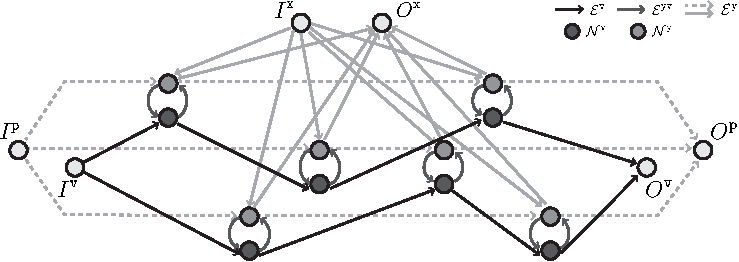
\includegraphics[scale=1.0]{figures/fullFlow.pdf}
	\caption{Here is the caption of this amazing figure, See also Table \protect\ref{tbl1}).}
	\label{FIG:1}
\end{figure}


\begin{table}[width=.9\linewidth,cols=4,pos=h]
\caption{This is a test caption. This is a test caption. This is a test
caption. This is a test caption.}\label{tbl1}
\begin{tabular*}{\tblwidth}{@{} LLLL@{} }
\toprule
Col 1 & Col 2 & Col 3 & Col4\\
\midrule
12345 & 12345 & 123 & 12345 \\
12345 & 12345 & 123 & 12345 \\
12345 & 12345 & 123 & 12345 \\
12345 & 12345 & 123 & 12345 \\
12345 & 12345 & 123 & 12345 \\
\bottomrule
\end{tabular*}
\end{table}

\section[Theorem and ...]{Theorem and theorem like environments}

{cas-sc.cls} provides a few shortcuts to format theorems and
theorem-like environments with ease. In all commands the options that
are used with the \verb+\newtheorem+ command will work exactly in the same
manner. {cas-sc.cls} provides three commands to format theorem or
theorem-like environments: 

\begin{verbatim}
 \newtheorem{theorem}{Theorem}
 \newtheorem{lemma}[theorem]{Lemma}
 \newdefinition{rmk}{Remark}
 \newproof{pf}{Proof}
 \newproof{pot}{Proof of Theorem \ref{thm2}}
\end{verbatim}


\newtheorem{theorem}{Theorem}

\begin{theorem}
For system (8), consensus can be achieved with 
$\|T_{\omega z}$ ...
\begin{eqnarray}\label{10}
....
\end{eqnarray}
\end{theorem}

\section{Bibliography}

Two bibliographic style files (\verb+*.bst+) are provided ---
{model1-num-names.bst} and {model2-names.bst} --- the first one can be
used for the numbered scheme. This can also be used for the numbered
with new options of {natbib.sty}. The second one is for the author year
scheme. When  you use model2-names.bst, the citation commands will be
like \verb+\citep+,  \verb+\citet+, \verb+\citealt+ etc. However when
you use model1-num-names.bst, you may use only \verb+\cite+ command.

\verb+thebibliography+ environment.  Each reference is a
\verb+\bibitem+ and each \verb+\bibitem+ is identified by a label,
by which it can be cited in the text:

\noindent In connection with cross-referencing and
possible future hyperlinking it is not a good idea to collect
more that one literature item in one \verb+\bibitem+.  The
so-called Harvard or author-year style of referencing is enabled
by the \LaTeX{} package {natbib}. With this package the
literature can be cited as follows:


\begin{enumerate}[\textbullet]
\item Parenthetical: \verb+\citep{WB96}+ produces (Wettig \& Brown, 1996).
\item Textual: \verb+\citet{ESG96}+ produces Elson et al. (1996).
\item An affix and part of a reference:
\verb+\citep[e.g.][Ch. 2]{Gea97}+ produces (e.g. Governato et
al., 1997, Ch. 2).
\end{enumerate}

In the numbered scheme of citation, \verb+\cite{<label>}+ is used,
since \verb+\citep+ or \verb+\citet+ has no relevance in the numbered
scheme.  {natbib} package is loaded by {cas-sc} with
\verb+numbers+ as default option.  You can change this to author-year
or harvard scheme by adding option \verb+authoryear+ in the class
loading command.  If you want to use more options of the {natbib}
package, you can do so with the \verb+\biboptions+ command.  For
details of various options of the {natbib} package, please take a
look at the {natbib} documentation, which is part of any standard
\LaTeX{} installation.

\appendix
\section{My Appendix}
Appendix sections are coded under \verb+\appendix+.

\verb+\printcredits+ command is used after appendix sections to list 
author credit taxonomy contribution roles tagged using \verb+\credit+ 
in frontmatter.

\printcredits

\bio{}
Author biography without author photo.
Author biography. Author biography. Author biography.
Author biography. Author biography. Author biography.
Author biography. Author biography. Author biography.
Author biography. Author biography. Author biography.
Author biography. Author biography. Author biography.
Author biography. Author biography. Author biography.
Author biography. Author biography. Author biography.
Author biography. Author biography. Author biography.
Author biography. Author biography. Author biography.
\endbio

\bio{figures/pic1}
Author biography with author photo.
Author biography. Author biography. Author biography.
Author biography. Author biography. Author biography.
Author biography. Author biography. Author biography.
Author biography. Author biography. Author biography.
Author biography. Author biography. Author biography.
Author biography. Author biography. Author biography.
Author biography. Author biography. Author biography.
Author biography. Author biography. Author biography.
Author biography. Author biography. Author biography.
\endbio

\bio{figures/pic1}
Author biography with author photo.
Author biography. Author biography. Author biography.
Author biography. Author biography. Author biography.
Author biography. Author biography. Author biography.
Author biography. Author biography. Author biography.
\endbio